%%%%%%%%%%%%%%%%%%%% book.tex %%%%%%%%%%%%%%%%%%%%%%%%%%%%%
%
% sample root file for the chapters of your "monograph"
%
% Use this file as a template for your own input.
%
%%%%%%%%%%%%%%%% Springer-Verlag %%%%%%%%%%%%%%%%%%%%%%%%%%


% RECOMMENDED %%%%%%%%%%%%%%%%%%%%%%%%%%%%%%%%%%%%%%%%%%%%%%%%%%%
\documentclass[envcountsame,envcountchap]{svmono}

% choose options for [] as required from the list
% in the Reference Guide, Sect. 2.2
\usepackage{geometry} 
\usepackage{makeidx}         % allows index generation
\usepackage{graphicx}        % standard LaTeX graphics tool
                             % when including figure files
\usepackage{multicol}        % used for the two-column index
\usepackage[bottom]{footmisc}% places footnotes at page bottom
\usepackage[italian]{babel}
\usepackage[utf8]{inputenc}

\usepackage{amsmath}%  %
\usepackage{amsfonts}%
\usepackage{amssymb}%es
\usepackage{mathtools}
\usepackage{clrscode}

\usepackage{hyperref}
\hypersetup{colorlinks=true, linkcolor=black} %per colorare i link

\DeclarePairedDelimiter{\abs}{\lvert}{\rvert}
\DeclarePairedDelimiter{\norma}{\lVert}{\rVert}

% etc.
% see the list of further useful packages
% in the Reference Guide, Sects. 2.3, 3.1-3.3

\makeindex             % used for the subject index
                       % please use the style svind.ist with
                       % your makeindex program


%%%%%%%%%%%%%%%%%%%%%%%%%%%%%%%%%%%%%%%%%%%%%%%%%%%%%%%%%%%%%%%%%%%%%

\begin{document}

\author{Roberto Melfi}
\title{Pattern Classification Lecture Notes\\
{\small Pattern Classification Course - A.Y. 2008/2009}}
\subtitle{In Memory of Prof. Alfredo Petrosino}
\maketitle

\frontmatter%%%%%%%%%%%%%%%%%%%%%%%%%%%%%%%%%%%%%%%%%%%%%%%%%%%%%%


%%%%%%%%%%%%%%%%%%%%%%% dedic.tex %%%%%%%%%%%%%%%%%%%%%%%%%%%%%%%%%
%
% sample dedication
%
% Use this file as a template for your own input.
%
%%%%%%%%%%%%%%%%%%%%%%%% Springer-Verlag %%%%%%%%%%%%%%%%%%%%%%%%%%

\thispagestyle{empty}
\vspace*{3.5cm}
\begin{flushright}

% write your text here
{\large Your dedication goes here}

\end{flushright}




%%%%%%%%%%%%%%%%%%%%%% pref.tex %%%%%%%%%%%%%%%%%%%%%%%%%%%%%%%%%%%%%
%
% sample preface
%
% Use this file as a template for your own input.
%
%%%%%%%%%%%%%%%%%%%%%%%% Springer-Verlag %%%%%%%%%%%%%%%%%%%%%%%%%%

\preface

%% Please write your preface here
Questi appunti sono stati scritti durante il corso di Riconoscimento e Classificazione di Forme tenuto dal Professore Alfredo Petrosino nell’anno accademico 2008/2009. Non sono semplici appunti, ma un’accurata sbobinatura di registrazioni delle sue lezioni unite a parti tradotte e sintetizzate del libro “Duda Hart” \cite{duda}. 
A distanza di circa dieci anni rendo pubblico questo lavoro, non per meriti, ma per tramandare per iscritto le lezioni del professore ai futuri studenti, se esistono questi appunti è solo grazie al suo corso, ho avuto soltanto la pazienza di trascriverli e organizzarli per poter preparare al meglio l’esame finale. \\
Gli appunti sono open source (\url{https://github.com/robmelfi/PatternRecognitionLectureNotes}), cosi da correggere eventuali errori di battitura e migliorare parti non abbastanza curate da parte mia. 
Il professore ha insegnato che la perfezione non esiste, ma un lavoro può essere sempre migliorato per tendere alla perfezione, questi appunti devono essere un punto di partenza per essere ampliati lasciando inalterate e mettendo in evidenza le parole del professore. 



%% Please "sign" your preface

\begin{flushright}\noindent
\hfill {\it Roberto Melfi}\\
\end{flushright}

\vspace{1cm}
\noindent Il ruolo di un professore è quello di essere guida e di insegnare la vita, oltre che la disciplina.
Gli studenti dell’Università Parthenope che hanno conosciuto il professore Alfredo Petrosino possono dire di aver avuto un’insegnante che ha ricoperto a pieno questo ruolo.
Grazie a lui abbiamo creato un gruppo di studio tra le scrivanie del CVPRLab che andava oltre i banchi universitari.
Durante tutto il percorso accademico abbiamo trascorso dei momenti intensi che ci han forgiato rendendoci le persone migliori che siamo oggi. Non gli saremo mai abbastanza riconoscenti per questo!
La sua prematura scomparsa è stata un fulmine a ciel sereno che ha riunito sotto lo stesso tetto, tutte le persone che lo conoscevano ed avevano lavorato con lui. Anche in questo momento è stato speciale dato ci siamo riuniti dopo anni in cui ognuno di noi ha intrapreso la sua strada.
Grazie di tutto prof!\\

“ti aspetterò comunque fruori alla porta 429 ... sarai semplicemente in ritardo ...”, il saluto di un suo caro allievo \emph{Enrico Balestrieri}.

\begin{flushright}\noindent
\hfill {\it Luca Russo}\\
\end{flushright}

\vspace{0.5cm}
Napoli, Gennaio 2020







\tableofcontents


\mainmatter%%%%%%%%%%%%%%%%%%%%%%%%%%%%%%%%%%%%%%%%%%%%%%%%%%%%%%%
%%%%%%%%%%%%%%%%%%%%%%%% part.tex %%%%%%%%%%%%%%%%%%%%%%%%%%%%%%%%%%
%
% sample part title
%
% Use this file as a template for your own input.
%
%%%%%%%%%%%%%%%%%%%%%%%% Springer-Verlag %%%%%%%%%%%%%%%%%%%%%%%%%%


\part{Parte Uno}

%%%%%%%%%%%%%%%%%%%%% chapter.tex %%%%%%%%%%%%%%%%%%%%%%%%%%%%%%%%%
%
% sample chapter
%
% Use this file as a template for your own input.
%
%%%%%%%%%%%%%%%%%%%%%%%% Springer-Verlag %%%%%%%%%%%%%%%%%%%%%%%%%%

\chapter{Bayesian Decision Theory}\label{teoriaBaesiana}
\label{teoriaBaesiana} % Always give a unique label
% use \chaptermark{}
% to alter or adjust the chapter heading in the running head

\section{Introduzione}
La Teoria delle decisioni baesiane è un fondamentale approccio statistico per il problema del \emph{Pattern Classification}. L'esempio preso in considerazione è quello di progettare un classificatore  che sia in grado di separare due specie di pesci: il branzino ed il salmone. Supponiamo che ci sia un operatore che sta osservando un nastro trasportatore sul quale scorrono queste due specie, l'osservatore trova difficile predire quale specie si presenterà all'arrivo del prossimo pesce. Denotiamo con $\omega$ lo \textbf{stato della natura}, poniamo $\omega = \omega_1$ per il branzino e $\omega = \omega_2$ per il salmone. Poichè lo stato della natura è imprevedibile allora consideriamo $\omega$ una variabile che deve essere descritta probabilisticamente. Si assume che siamo a conoscenza delle \textbf{probabilità a priori}, denotiamo con $P(\omega_1)$ la probabilità che il prossimo pesce sia un branzino e con $P(\omega_2)$ la probabilità che il prossimo pesce sia un salmone, se si assume che non ci siano altre tipologie di pesci allora la somma di $P(\omega_1)$ e $P(\omega_2)$ è uguale ad uno. Le due probabilità possono essere ricavate statisticamente sulla storia passata, quindi una regola di decisione potrebbe essere quella di scegliere $\omega_1$ se $P(\omega_1) > P(\omega_2)$, altrimenti viene scelto $\omega_2$. Questa regola potrebbe avere senso se prendiamo in considerazione soltanto due tipologie di classi, infatti potrebbe risultare strano se si applica questa regola quando c'è da classificare più di due classi. Nella maggior parte delle circostanze non è utile prendere decisioni con così poche informazioni. Nella classificazione tra le due specie di pesci, per esempio possiamo prendere in considerazione la misura della luminanza
$x$ per migliorare il nostro classificatore. Ogni pesce avrà una luminanza diversa ed è possibile esprimere questa variabile in termini probabilistici, si considera $x$ come una variabile casuale la cui distribuzione dipende dallo stato della natura ed è espressa come $p(x|\omega)$ che viene definita funzione della densità di probabilità condizionale, ovvero la funzione della densità di probabilità per $x$ dato lo stato della natura $\omega$. Quindi la differenza tra $p(x|\omega_1)$ e  $p(x|\omega_2)$ descrive la differenza di luminanza tra la popolazione dei branzini e quella dei salmoni (fig. \ref{cpdf}).


\begin{figure}
\centering
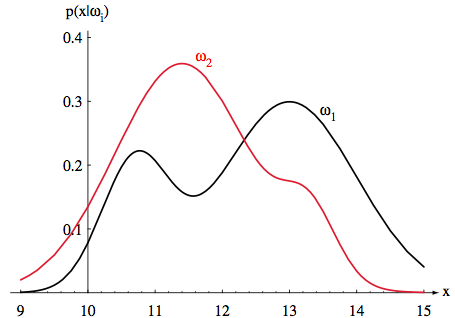
\includegraphics[scale=0.6]{img/cpdf.png}
\caption{Funzione di densità della probabilità condizionate delle due classi di pesci per la caratteristica della luminanza $x$}
\label{cpdf}
\end{figure}
\noindent Supponiamo che siamo a conoscenza di entrambi le probabilità a priori $P(\omega_j)$ e delle funzioni di densità della probabilità condizionata $p(x|\omega_j)$ per $j = 1,2$. Supponiamo che arrivi un pesce sul nastro trasportatore e misuriamo la luminanza $x$. Qui entra in gioco la regola di Bayes. Conosciamo $p(x|\omega_j) = p(x \cap \omega_j) / P(\omega_j)$, il nostro obiettivo è quello di calcolare $P(\omega_j | x)$, ovvero la probabilità di appartenenza alla classe $\omega_j$ dato la misura di luminanza $x$ rilevata. $P(\omega_j | x) = P(x \cap \omega_j) / p(x)$, quindi per il teorema della moltiplicazione
\begin{gather}
p(\omega_j \cup x) = p(x|\omega_j) P(\omega_j)\\
p(\omega_j \cup x) = P(\omega_j|x ) p(x)
\end{gather}
riarrangiando i termini otteniamo la risposta al nostro quesito mediante la regola di Bayes
\begin{equation}
P(\omega_j|x) = \frac{p(x|\omega_j) P(\omega_j)}{p(x)}
\end{equation}
dove nel caso di due categorie
\begin{equation}
p(x) = \sum_{j=1}^2 p(x|\omega_j) P(\omega_j)
\end{equation}
La formula di Bayes può essere espressa informalmente  dicendo che
\begin{equation}
\text{Posterior} = \frac{\text{likelihood (verosomigianza)} \times \text{prior}}{\text{evicence}}
\end{equation}
La formula di Bayes mostra che osservando il valore di $x$ possiamo convertire la \textbf{probabilità a priori} $P(\omega_j)$ nella \textbf{probabilità a posteriori} $P(\omega_j|x)$, ovvero la probabilità di avere la classe $\omega_j$ dato il valore $x$ misurato. Chiamiamo $P(x|\omega_j)$ \emph{\textbf{likelihood}} (verosomiglianza) di $\omega_j$ rispetto ad $x$. $p(x)$ invece è il fattore evidenza e può essere visto come un fattore di scala che garantisce che la somma delle probabilità a posteriori sia uguale ad uno. La variazione di $P(\omega_j|x)$ è illustrata in figura \ref{prob_post} per il caso con $P(\omega_1) = 2/3$ e $P(\omega_2) = 1/3$.
\begin{figure}
\centering
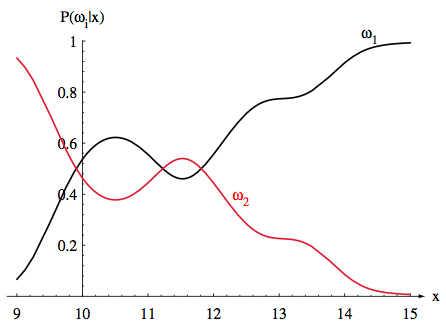
\includegraphics[scale=0.6]{img/prob_post.png}
\caption{Probabilità posteriori calcolate per le probabilità a priori $P(\omega_1) = 2/3$ e $P(\omega_2) = 1/3$ per le funzioni di densità di probabliità condizionata mostrate in fig. \ref{cpdf}}
\label{prob_post}
\end{figure}
\noindent Quindi nel caso di due classi è ovvio scegliere $\omega_1$ se $P(\omega_1|x) > P(\omega_2|x)$ e viceversa. Per giustificare questa procedura di decisione è opportuno calcolare la probabilità di errore. Qualsiasi sia la variabile $x$ osservata la probabilità di errore è

\[
P(error | x)=
\begin{cases}
P(\omega_1|x) & \text{se dicidiamo $\omega_2$} \\
P(\omega_2|x) & \text{se dicidiamo $\omega_1$} 
\end{cases}
\]


\section{Teoria delle decisioni baesiane -- Continuous Features}

In questo paragrafo verrà formalizzata l'idea descritta nel paragrafo precedente e viene generalizzata in modo tale da 
\begin{itemize}
\item Consentire l'uso di più caratteristiche
\item Consentire la classificazione tra più classi
\item Consentire l'esecuzione di altre azioni semplicemente decidendo lo stato della natura
\item Introducendo una funzione di perdita più generale della probabilità d'errore
\end{itemize}
Per quanto riguarda il primo punto basta semplicemente sostituire lo scalare $x$ con un \emph{feature vector} (vettore delle caratteristiche) $\mathbf{x}$, dove $\mathbf{x}$ è un vettore a $d$ dimensioni nello spazio Euclideo 	$\mathbf{R}^d$, chiamato \emph{feature space} (spazio delle carateristiche), quindi analogamente al caso precedente denotiamo con $p(\mathbf{x}|\omega_j)$ la funzione di densità della probabilità condizionata per $\mathbf{x}$. Come prima, $P(\omega_j)$ descrive la probabilità a priori per le varie classi $\omega_j$, quindi la probabilità a posteriori può essere ottenuta mediante la formula di Bayes:
\begin{equation}
P(\omega_j| \mathbf{x}) = \frac{p(\mathbf{x}|\omega_j) P(\omega_j)}{p(\mathbf{x})}
\end{equation}
in questo caso l'evidenza viene calcolata come segue
\begin{equation}
p(x) = \sum_{j=1}^c p(\mathbf{x} | \omega_j) P(\omega_j)
\end{equation}
Le formule appena descritte possono essere utilizzate anche per estendere la classificazione tra $c$ classi.\\

\noindent In generale classificare significa anche prendere una decisione dell'azione da intraprendere. Denotiamo con $\{\omega_1, \dots, \omega_c\}$ un insieme finito di $c$ categorie e con $\{\alpha_1, \dots, \alpha_a\}$ un insieme finito di $a$ possibili azioni da intraprendere, inoltre denotiamo con $\lambda(\alpha_i|\omega_j)$ la funzione di perdita che descrive la perdita o il costo al quale si incorre nel caso venga scelta l'azione $\alpha_i$ quando si è scelta la classe $\omega_j$. Possiamo definire \emph{rischio} la perdita $R(\alpha_i|\mathbf{x})$, ovvero la perdita che si ha nel caso si sia scelto di eseguire l'azione $\alpha_i$ dato il vettore delle caratteristiche $\mathbf{x}$ e viene calcolata come segue
\begin{equation}\label{risk}
R(\alpha_i | \mathbf{x}) = \sum_{j=1}^c \lambda(\alpha_i | \omega_j) P(\omega_j | \mathbf{x})
\end{equation}
Qualunque sia l'osservazione $\mathbf{x}$, è possibile minimizzare la perdita selezionando l'azione che minimizza il rischio. Un problema è quello di trovare una regola di decisione che minimizza il rischio totale. Una regola di decisione generale è la funzione $\alpha(\mathbf{x})$ che ci dice quale azione eseguire per ogni possibile osservazione. Quindi per ogni osservazione $\mathbf{x}$ è associata un unica azione $\alpha_1, \dots, \alpha_a$. Il rischio associato ad una data regola di decisione misura la perdita attesa quando tale regola venisse adottata su tutte le osservazioni $\mathbf{x}$
\begin{equation}
R = \int R(\alpha(\mathbf{x}) | \mathbf{x}) p(\mathbf{x}) \ d\mathbf{x}
\end{equation}
per minimizzare il rischio totale allora si calcolano tutti i rischi $R(\alpha_i | \mathbf{x})$ per $i=1, \dots, a$ e si sceglie l'azione $\alpha_i$ per la quale il rischio $R(\alpha_i | \mathbf{x})$ è minimo.

\subsection{Classificazione tra due categorie}
Consideriamo un problema di classificazione tra soltanto due categorie. Quindi abbiamo l'azione $\alpha_1$ che corrisponde alla decisione presa se il classificatore da come risultato $\omega_1$ e l'azione $\alpha_2$ che corrisponde alla decisione presa se il classificatore restituisce $\omega_2$. Per semplificare la notazione poniamo la funzione di perdita $\lambda_{ij} = \lambda(\alpha_i, \omega_j)$, che come abbiamo detto corrisponde alla perdita nel caso si esegue l'azione $\alpha_i$ scelta la categoria $\omega_j$. Dall'equazione \ref{risk} otteniamo il rischio
\begin{gather}
R(\alpha_1 | \mathbf{x}) =  \lambda_{11} P(\omega_1 | \mathbf{x}) + \lambda_{12} P(\omega_2 | \mathbf{x})\\
R(\alpha_2 | \mathbf{x}) =  \lambda_{21} P(\omega_1 | \mathbf{x}) + \lambda_{22} P(\omega_2 | \mathbf{x})
\end{gather}
Ci sono molti metodi per esprimere la regola di decisione del minimo rischio. La regola fondamentale è quella di decidere $\omega_1$ se $R(\alpha_1 | \mathbf{x}) < R(\alpha_2 | \mathbf{x})$. Invece in termini di probabilità a posteriori otteniamo da semplici sostituzioni la seguente regola decidendo $\omega_1$ se
\begin{equation}
(\lambda_{21} - \lambda_{11}) P(\omega_1 | \mathbf{x}) > (\lambda_{12} - \lambda_{22}) P(\omega_2 | \mathbf{x})
\end{equation}
 Invece, utilizzando la regola di Bayes possiamo sostituire le probabilità a posteriori con le probabilità a priori e le funzioni di densità di probabilità condizionata, ciò equivale a decidere $\omega_1$ se
\begin{equation}
(\lambda_{21} - \lambda_{11}) p(\mathbf{x}|\omega_1) P(\omega_1) > (\lambda_{12} - \lambda_{22}) p(\mathbf{x}|\omega_2) P(\omega_2)
\end{equation}
Un altra alternativa, assumendo $\lambda_{21} > \lambda_{11}$, è quella di decidere $\omega_1$ se
\begin{equation}
\frac{p(\mathbf{x}|\omega_1)}{p(\mathbf{x}|\omega_2)} > \frac{\lambda_{12} - \lambda_{22}}{\lambda_{21} - \lambda_{11}} \ \frac{P(\omega_2)}{P(\omega_1)}
\end{equation}
Questa regola di decisione si focalizza sulla dipendenza $\mathbf{x}$ dalla densità della probabilità condizionate. Possiamo considerare $p(\mathbf{x}|\omega_1) / p(\mathbf{x}|\omega_2)$ il rapporto di verosomiglianza (\emph{likelihood ratio}). Questa regola di decisione baesiana può essere utilizzata per decidere $\omega_1$ se il tasso di verosomiglianza supera una determinata soglia rendendo così la regola indipendente dall'osservazione $\mathbf{x}$

\section{Classificazione con tasso di errore minimo}
Nel problema della classificazione ogni stato è generalmente associato ad una classe, e l'azione $\alpha_i$ viene associata allo stato $\omega_i$. In generale se l'azione è $\alpha_i$ e lo stato è $\omega_j$ allora la decisione è corretta se $i = j$ ed è sbagliata se $i \neq j$. Per evitare gli errori allora è opportuno cercare regole di decisione che minimizzano gli errori o tasso di errore (\emph{error rate}). La funzione di perdita in questo caso è chiamata simmetrica o funzione di perdita \emph{zero-one},
\[
\lambda(\alpha_i, \omega_j)=
\begin{cases}
0 & \text{se} \ i = j\\
1 & \text{se} \ i \neq j 
\end{cases} 
\quad \quad \quad
i,j = 1, \dots, c.
\]
Questa funzione non assegna perdita ad una decisione corretta mentre assegna una perdita pari a uno quando la decisione è sbagliata. Il rischio quindi è calcolato come segue
\begin{equation}
\begin{split}
R(\alpha_i | \mathbf{x}) &= \sum_{j=1}^c \lambda(\alpha_i | \omega_j ) P(\omega_j | \mathbf{x}) \\
&= \sum_{j \neq i} P(\omega_j | \mathbf{x})\\
&= 1 - P(\omega_i | \mathbf{x})
\end{split}
\end{equation}
Quindi per minimizzare il tasso di errore dobbiamo scegliere l'indice $i$ che massimizza la probabilità a posteriori (MAP) $P(\omega_i | \mathbf{x})$. In altre parole per il tasso di errore minimo decidiamo $\omega_i$ se
\begin{equation}
P(\omega_i | \mathbf{x}) > P(\omega_j | \mathbf{x}) \quad \quad \quad \text{per tutti} \quad  j \neq i
\end{equation}

\section{Classificatori, Funzioni discriminanti e superfici di decisione}
\subsection{Il caso multicategoria}\label{casoMulticategoria}
Ci sono tanti modi diversi per rappresentare un classificatore di pattern. Uno dei più comunemente usati si basa sulle \emph{funzioni discriminanti} $g_i(\mathbf{x}), \ i = 1, \dots, c.$ Il classificatore ci dice di assegnare il vettore delle caratteristiche $\mathbf{x}$ alla classe $\omega_j$ se
\begin{equation}
g_i(\mathbf{x}) > g_j(\mathbf{x}) \ \ \ \text{per ogni} \ j \neq i
\end{equation}
Il classificatore può essere visto come una rete di macchine che calcolano le $c$ funzioni discriminanti e sceglie la categoria corrispondente alla funzione discriminante che ha restituito una risposta maggiore.
\begin{figure}
\centering
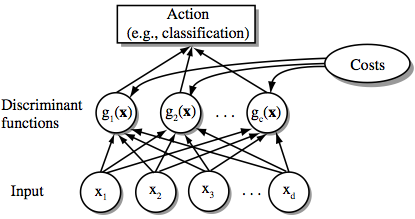
\includegraphics[scale=0.7]{img/network.png}
\caption{La struttura funzionale di comune classificatore di pattern la quale include $d$ input e $c$ funzioni discriminanti $g_i(\mathbf{x})$. Viene determinato quale dei valori discriminanti è il massimo e viene classificato il pattern di input.}
\label{network}
\end{figure}
In figura \ref{network} possiamo osservare un classificatore basato su una rete di funzioni discriminanti.
Un classificatore Baesiano  è semplicemente e naturalmente rappresentato in questo modo. Per un caso più generale, dove viene preso in considerazione anche il rischio, possiamo dire che $g_i(\mathbf{x}) = -R(\alpha_i|\mathbf{x})$, poiché la funzione discriminante massima corrisponde al minimo rischio. Invece per il caso a minimo tasso di errore possiamo semplificare ulteriormente le cose considerando $g_i(\mathbf{x}) = P(\omega_i|\mathbf{x})$, in questo modo affermiamo che la funzione discriminante massima corrisponde alla massima probabilità a posteriori (MAP). La scelta della funzione discriminante non è unica, è possibile moltiplicare tutte le funzioni discriminanti con una costante positiva senza influenzare la decisione. Inoltre, se sostituiamo ogni $g_i(\mathbf{x})$ con $f(g_i(\mathbf{x}))$, dove $f(\cdot)$ è una funzione monotona crescente, il risultato della classificazione resta invariato. Questa osservarzione comporta il vantaggio di significative semplificazioni analitiche e computazionali. In particolare, per la classificazione a tasso minimo di errore, qualsiasi delle seguenti scelte danno la stessa risposta di classificazione, ma alcune possono risultare più semplici da capire o da calcolare rispetto alle altre:
\begin{gather}
g_i(\mathbf{x}) = P(\omega_i|\mathbf{x}) = \frac{p(\mathbf{x}|\omega_i) P(\omega_i)}{\sum_{j=1}^c p(\mathbf{x} | \omega_j) P(\omega_j)}\\
g_i(\mathbf{x}) = p(\mathbf{x}|\omega_i) P(\omega_i)\\
g_i(\mathbf{x}) = \ln p(\mathbf{x}|\omega_i) + \ln P(\omega_i)
\end{gather} 
dove con $\ln$ indichiamo il logaritmo naturale.
Come abbiamo visto le funzioni discriminanti possono essere descritte in vari modi ma le regole di decisione sono equivalenti. Lo scopo di qualsiasi regola di decisione è quello di dividere lo spazio delle caratteristiche in $c$ \emph{regioni di decisione}, $\mathcal{R}_1, \dots, \mathcal{R}_c$. Se $g_i(\mathbf{x}) > g_j(\mathbf{x})$ per ogni $j \neq i$, allora $\mathbf{x}$ è in $\mathcal{R}_i$ e la regola di decisione assegna $\mathbf{x}$ a $\omega_i$. Le regioni sono separate dai \emph{decision boundaries} che possiamo osservare in fig. \ref{decisionBoundaries}
\begin{figure}
\centering
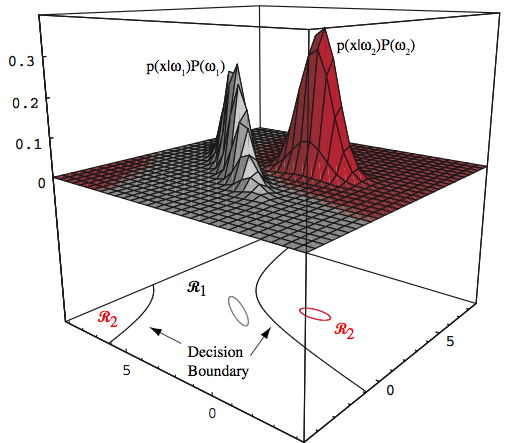
\includegraphics[scale=0.6]{img/decisionBoundaries.png}
\caption{Classificatore tra due categoria in due dmensioni, le densità di probabilità sono gaussiane, i bordi di decisione consistono in due iperbole e la regione di decisione $\mathcal{R}_2$ non è semplicemente connessa}
\label{decisionBoundaries}
\end{figure}

\subsection{Il caso a due categorie}
Il caso a due categorie è un caso speciale del caso multigategoria, e riceve un trattamento separato. Prende anche il nome speciale \emph{dichotomizer}. Invece di usare le due funzioni discriminanti $g_1$ e $g_2$ e assegnare $\mathbf{x}$ a $\omega_1$ se $g_1 > g_2$, è comune definire una singola funzione discriminante 
\begin{equation}
g(\mathbf{x}) = g_1(\mathbf{x}) - g_2(\mathbf{x})
\end{equation}
usando la seguente regola di decisione: Si decide $\omega_1$ se $g(\mathbf{x}) > 0$; altrimenti si decide $\omega_2$. Perciò il \emph{dichotomizer} può essere visto come una macchina che calcola una singola funzione discriminante $g(\mathbf{x})$ e classifica $\mathbf{x}$ in base al segno del risultato.
\clearpage
\section{La distribuzione normale}
La struttura di un classificatore baesiano è determinata dalle funzioni di distribuzione di probabilità condizionata $p(\mathbf{x}|\omega_i)$ e dalle probabilità a priori $P(\omega_i)$. Tra le tante distribuzioni di densità hanno avuto particolare importanza la funzione di distribuzione normale e multivariata di Gauss, proprio per la loro semplice trattabilità analitica. Inoltre la distribuzione multivariata è anche un modello appropriato per situazioni importanti, vale a dire il caso in cui il vettore delle caratteristiche $\mathbf{x}$ per una data classe $\omega_i$ sono valori continui. In questa sezione viene fornita una breve esposizione delle distribuzioni suddette focalizzandoci sulle proprietà che hanno maggiore interesse per il problema della classificazione.  Incominciamo con un richiamo della definizione del valore atteso di una funzione $f(x)$ definita per la densità $p(x)$
\begin{equation}
\varepsilon [ f(x) ] \equiv \int_{-\infty}^{\infty} f(x) p(x) \ dx
\end{equation}
Se il valore appartiene ad un insieme di punti discreti $\mathcal{D}$ allora la formula si riduce ad una semplice sommatoria
\begin{equation}
\varepsilon [ f(x) ] = \sum_{x \in \mathcal{D}} f(x) P(x)
\end{equation}

\subsection{Distribuzione normale unidimensionale}
Iniziamo col descrivere la distribuzione normale di Gauss unidimensionale,
\begin{equation}
p(x) = \frac{1}{\sqrt{2\pi} \sigma} \exp  \left [ -\frac{1}{2}  \left (  \frac{x - \mu}{\sigma} \right )^2 \right  ]
\end{equation}
per la quale il valore atteso $x$ è calcolato come segue
\begin{equation}
\mu \equiv \varepsilon [x] = \int_{-\infty}^{\infty} xp(x) \ dx
\end{equation}
e la varianza è
\begin{equation}
\sigma^2 \equiv \varepsilon [(x - \mu)^2] = \int_{-\infty}^{\infty} (x - \mu)^2 p(x) \ dx
\end{equation}
La distribuzione normale unidimensionale è caratterizzata da due parametri: la media $\mu$ e la varianza $\sigma^2$, in generale vengono anche chiamati rispettivamente momento del primo ordine e momento del secondo ordine. Per semplicità la distribuzione viene indicata con $N(\mu, \sigma^2)$, un esempio di distribuzione è mostrato in figura \ref{gauss}.\\
\begin{figure}
\centering
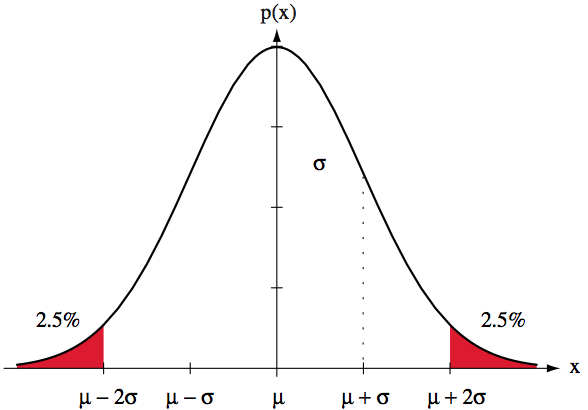
\includegraphics[scale=0.5]{img/gauss.png}
\caption{Distribuzione di Gauss}
\label{gauss}
\end{figure}

\paragraph{Alcune osservazioni}
La funzione è definita su tutto l’asse reale, non è mai né nulla né negativa. Essa è simmetrica rispetto all’asse $y=\mu$  e tende a zero al tendere di $x$ all’infinito. Essa dunque assegna una probabilità a features che hanno range potenzialmente infinito. Inoltre la probabilità assegnata è la stessa per valori equidistanti (sia a destra come a sinistra) da $\mu$. La massima probabilità viene assegnata al valore $\mu$ che si chiama anche valore centrale della distribuzione.\\
Il parametro $\sigma$ serve a determinare quanto è “larga” o “svasata” la campana della gaussiana. Valori grandi per $\sigma$ indicano una “dispersione” notevole dei dati attorno al valore centrale, un valore piccolo invece indica che i dati sono tutti “vicini” al valore centrale. Tale “interpretazione” per il parametro $\sigma$ viene dal fatto che se si calcola l’integrale definito tra $\mu - 2\sigma$ e $\mu + 2\sigma$ si ottiene 0.95. Cioè la popolazione rappresentata dal modello gaussiano si addensa nell’intervallo centrato in $\mu$ e largo $4\sigma$ al $95\%$. Il restante $5\%$ forma le cosidetta “code” della distribuzione.\\

\noindent Trasformazioni lineare di gaussiane: se moltiplico o divido una gaussiana per un valore essa resta sempre una gaussiana, la gaussiana soddisfa il fattore di scaling. Se si sommano le gaussiane si ottiengono mixture di gaussiane, che non sono gaussiane ma distribuzioni di probablità, un insieme di tante campane.\\ 

\noindent Vi è un importante rapporto tra la distribuzione normale e l'entropia\footnote{L'entropia misura la quantità di incertezza o informazione presente in un segnale aleatorio. Da un altro punto di vista l'entropia è la minima complessità descrittiva di una variabile aleatoria, ovvero il limite inferiore della compressione dei dati.}. L'entropia di una distribuzione è calcolata come segue
\begin{equation}
H(p(x)) = - \int p(x) \ln p(x) \ dx
\end{equation}
ed è misurata in \emph{nats}; se invece viene utilizzato il logaritmo di base due, quindi $\log_2$, allora viene misurata in \emph{bit}. L'entropia misura l'incertezza fondamentale nei valori dei punti scelti a caso da una distribuzione.\\

\noindent \emph{Teorema del limite centrale}: L’effetto aggregato ottenuto sommando un grande numero di piccoli contributi random (generati da distribuzioni uniformi) porta ad una distribuzione di Gauss.

\subsection{Distribuzione Multivariata}
La distribuzione Multivariata $d$ dimensionale è scritta come segue
\begin{equation}\label{distribuzioneMultivariata}
p(\mathbf{x}) = \frac{1}{(2\pi)^{d/2} \abs{\mathbf{\Sigma}}^{1/2}} \exp \left [ - \frac{1}{2} (\mathbf{x} - \mathbf{\mu})'  \mathbf{\Sigma}^{-1} (\mathbf{x} - \mathbf{\mu}) \right ]
\end{equation}
dove $\mathbf{x}$ è un vettore colonna, $\mathbf{\mu}$ è il vettore media, $\mathbf{\Sigma}$ è la matrice di covarianza $d \times d$, la matrice di covarianza non è altro che la media dei prodotti degli scarti, $\abs{\mathbf{\Sigma}}$ e $ \mathbf{\Sigma}^{-1}$ sono rispettivamente il determinante e l'inversa. Inoltre denotiamo con $(\mathbf{x} - \mathbf{\mu})' $ la trasposta di $(\mathbf{x} - \mathbf{\mu})$. L'operazione di sottrarre ad ogni $\mathbf{x}$ la propria media $\mathbf{\mu}$ prende il nome di \emph{whitening} (sbiancamento), perchè se si sottrae ad ogni $\mathbf{x}$ la propria media $\mathbf{\mu}$ allora la gaussiana è centrata in 0. Se si vuole ottenere una gaussiana standardizzata bisogna portare la media uguale a zero e la varianza uguale a uno, per fare ciò basta sottrarre la media e dividere per la varianza.
\begin{equation}
Z = \frac{X-\mu}{\sigma}
\end{equation}
La notazione per il prodotto interno è
\begin{equation}
\mathbf{a'b} = \sum_{i=1}^d a_ib_i
\end{equation}
che per semplicità spesso viene chiamato prodotto puntuale. La distribuzione normale spesso viene indicata con $N(\mathbf{\mu, \Sigma})$.
Formalmente la media è calcolata come segue
\begin{equation}
\mathbf{\mu} \equiv \varepsilon[\mathbf{x}] = \int \mathbf{x} p(x) \  d \mathbf{x}
\end{equation}
e la matrice di covarianza 
\begin{equation}
\mathbf{\Sigma} \equiv \varepsilon[(\mathbf{x-\mu)(x-\mu)'}] = \int (\mathbf{x-\mu)(x-\mu)'} p(\mathbf{x})  \  d \mathbf{x}
\end{equation} 
è possibile calcolare il vettore media e la matrice di covarianza anche componente per componente. Nel caso della media, se $x_i$ è la $i$-esima componente di $\mathbf{x}$, se $\mu_i$ è la $i$-esima componente di $\mathbf{\mu}$ e $\sigma_{ij}$ è la $ij$-esima componente di $\mathbf{\Sigma}$ allora
\begin{equation}
\mu_i = \varepsilon[x_i]
\end{equation}
e
\begin{equation}
\sigma_{ij} = \varepsilon[(x_i - \mu_i) (x_j - \mu_j) ]
\end{equation}
Gli elementi $\sigma_{ij}$ della matrice di covarianza hanno una precisa interpretazione. Gli elementi sulla diagonale rappresentano le varianze di ciascuna delle componenti del vettore $\mathbf{x}$. L’elemento $\sigma_{ij}$ se è positivo ci dice che la feature $i$ e la feature $j$ sono correlate positivamente (se una cresce, statisticamente cresce anche l’altra), se è negativo il contrario. Se è nullo ci dice che le feature non sono correlate o che sono statisticamente indipendenti.\\

\noindent I punti si trovano in uno spazio, per semplicità prendiamo lo spazio bidimensionale $x_1$ e $x_2$, come possiamo osservare in figura \ref{gauss1} i campioni giacciono nella nuvola centrata nella media, il luogo dei punti sono degli ellissoidi, dato che stiamo guardando la gaussiana dall'alto.
\begin{figure}
\centering
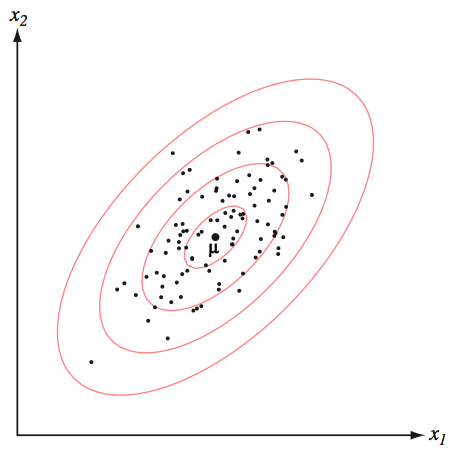
\includegraphics[scale=0.5]{img/gauss1.png}
\caption{Esempio di gaussiana bidimensionale, i campioni giacciono nella nuvola centrata nella media $\mu$}
\label{gauss1}
\end{figure}
Nel caso bidimensionale la gaussiana avrà due varianze, una nella direzione $x_1$ e l'altra nella direzione $x_2$, se le due varianze sono uguali allora la curva di livello è una circonferenza, se invece sono diverse allora è un ellisse. La cosa interessante è che tutti i punti che ricadono nella curva di livello soddisfano questa equazione
\begin{equation}
r^2 = (\mathbf{x- \mu)' \Sigma^{-1} (x- \mu)}
\end{equation}
con $r$ costante. Questa quantità è denominata distanza di \emph{Mahalanobis} da $\mathbf{x}$ a $\mathbf{\mu}$. Se la matrice di covarianza è una matrice diagonale dove sulla diagonale principale ha tutte varianze uguali, allora la distanza diventa euclidea. Un' altra particolarità interessa anche gli autovalori e gli autovettori della matrice di covarianza. Prima di vederla facciamo un breve richiamo sugli Autovalori e Autovettori di una matrice.

\paragraph{Autovalori e Autovettori}
Data la matrice $\mathbf{A}$ gli autovalori si calcolano 
\begin{equation}
\mathbf{A} \mathbf{x} = \lambda \mathbf{x}
\end{equation}
che può essere riscritta come
\begin{equation}
(\mathbf{A} - \lambda \mathbf{I})\mathbf{x} = \mathbf{0}
\end{equation}
dove $\lambda$ sono gli autovalori. Se $\mathbf{A}$ è una matrice quadrata $d \times d$ allora ho $d$ autovalori e $d$ autovettori. Gli autovalori di una matrice danno l'idea dell'energia e sono direttamente proporzionali alle varianze di ogni dimensione, gli autovettori invece sono i vettori che generano un nuovo spazio.\\

\noindent Ritornando alla gaussiana bidimensionale, la cosa interessante è che l'asse maggiore dell'ellisse è uguale alla varianza più grande, mentre l'asse minore è uguale alla varianza più piccola, più precisamente l'asse maggiore è lunga quanto l'autovalore più grande della matrice di covarianza e l'asse minore è lunga quanto l'autovalore più piccolo della matrice di covarianza, inoltre la direzione dell' asse maggiore è l'autovettore corrispondente all'autovalore più grande, mentre la direzione dell'asse minore è l'autovettore corrispondente all'autovalore più piccolo. 

%\paragraph{Trasformazione lineare di funzioni normali e \emph{Whitening (sbiancamento)}}
%Sia $\mathbf{A}$ una matrice $d \times k$ (generalmente è utile pensare a $d$ come più piccolo di $k$). Mediante tale matrice si può trasformare ogni vettore di $k$ componenti in un vettore di $d$ componenti facendo il prodotto $\mathbf{A'x}$. Componendo questa trasformazione con la distribuzione normale $N\mathbf{(\mu,\Sigma})$ si ottiene una nuova distribuzione normale $N(\mathbf{A'\mu, A' \Sigma A})$ come mostrato in figura \ref{sbianc} 
%\begin{figure}
%\centering
%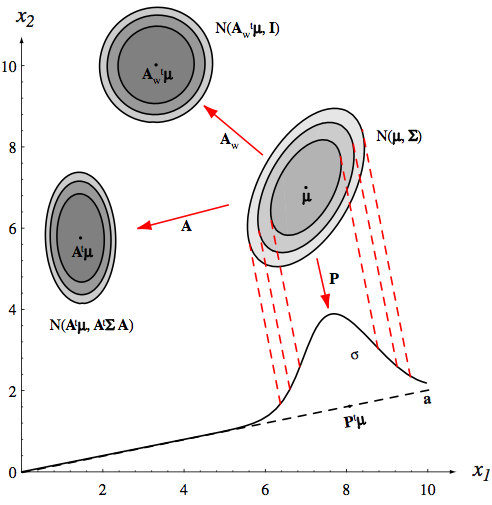
\includegraphics[scale=0.5]{img/sbiancamento.png}
%\caption{Trasformazione lineare}
%\label{sbianc}
%\end{figure}
%Particolarmente utile è la trasformazione con la matrice $k \times k$ \ $\mathbf{A_w}$ (matrice di \emph{whitening} o sbiancamento) che si ottiene come segue:\\ 
%Si calcolano gli autovalori e gli autovettori della matrice di covarianza $\mathbf{\Sigma}$. Si raccolgono gli autovalori in una matrice diagonale $\mathbf{\Lambda}$ e si dispongono nel medesimo ordine come colonne gli autovettori (ortogonali tra loro e normalizzati) in una matrice $\mathbf{\Phi}$. Allora $\mathbf{A_w = \Phi \Lambda}^{-1/2}$.
%La trasformazione con la matrice di \emph{whitening} trasforma la distribuzione gaussiana di partenza (tipicamente ellissoidale orientata in maniera arbitraria nello spazio) in una distribuzione “sferica” con covarianza eguale alla matrice identica. Questo può semplificare in molti casi l’analisi. Ne riparleremo quando affronteremo lo studio della PCA.

\section{Funzioni Discriminanti per la Distribuzione Normale}
Nella sezione \ref{casoMulticategoria} abbiamo visto che un classificatore a minimo tasso di errore può essere espresso usando le funzioni discriminanti
\begin{equation}\label{funzioneDiscriminante}
g_i(\mathbf{x}) = \ln p(\mathbf{x}|\omega_i) + \ln P(\omega_i)
\end{equation}
L'espressione può essere rivalutata se la distribuzione di probabilità $p(\mathbf{x}|\omega_i)$ è una distribuzione multivariata eq. (\ref{distribuzioneMultivariata}). Andando a sostituire all'interno dell' eq. (\ref{funzioneDiscriminante}) e utilizzando le prorpietà dei logaritmi otteniamo:

\begin{equation}\label{fun}
\begin{split}
g_i(\mathbf{x}) &= 
\ln \left \{  
\frac{1}{(2\pi)^{d/2} \abs{\mathbf{\Sigma}_i}^{1/2}} \exp \left [ - \frac{1}{2} (\mathbf{x} - \mathbf{\mu})'  \mathbf{\Sigma}_i^{-1} (\mathbf{x} - \mathbf{\mu}_i) \right ]  
\right \}
+ \ln P(\omega_i) \\
&= \ln \frac{1}{(2\pi)^{d/2} \abs{\mathbf{\Sigma}_i}^{1/2}} + \ln \exp \left [ - \frac{1}{2} (\mathbf{x} - \mathbf{\mu})'  \mathbf{\Sigma}_i^{-1} (\mathbf{x} - \mathbf{\mu}_i) \right ] + \ln P(\omega_i)\\
&= \ln 1 - \ln (2\pi)^{d/2} \abs{\mathbf{\Sigma}_i}^{1/2} - \frac{1}{2} (\mathbf{x} - \mathbf{\mu})'  \mathbf{\Sigma}_i^{-1} (\mathbf{x} - \mathbf{\mu}_i) + \ln P(\omega_i)\\
&= - \left( \frac{d}{2} \ln 2\pi + \frac{1}{2} \ln \abs{\mathbf{\Sigma}} \right) - \frac{1}{2} (\mathbf{x} - \mathbf{\mu})'  \mathbf{\Sigma}_i^{-1} (\mathbf{x} - \mathbf{\mu}_i) + \ln P(\omega_i)\\
&= - \frac{1}{2} (\mathbf{x} - \mathbf{\mu})'  \mathbf{\Sigma}_i^{-1} (\mathbf{x} - \mathbf{\mu}_i) - \frac{d}{2} \ln 2\pi - \frac{1}{2} \ln \abs{\mathbf{\Sigma}} + \ln P(\omega_i) 
%&=  \left [- \frac{1}{2} (\mathbf{x} - \mathbf{\mu}_i)'  \mathbf{\Sigma}_i^{-1} (\mathbf{x} - \mathbf{\mu}_i) \right ] \ln \left ( \frac{1}{(2\pi)^{d/2} \abs{\mathbf{\Sigma}_i}^{1/2}} e \right ) + \ln P(\omega_i) \\
%&= \left [- \frac{1}{2} (\mathbf{x} - \mathbf{\mu}_i)'  \mathbf{\Sigma}_i^{-1} (\mathbf{x} - \mathbf{\mu}_i) \right ] \ln \left ( 2\pi^{-d/2} \right ) + \ln \left ( \abs{\mathbf{\Sigma}_i}^{-1/2} \right ) + \ln e + \ln P(\omega_i)\\
%&= - \frac{1}{2} (\mathbf{x} - \mathbf{\mu}_i)'  \mathbf{\Sigma}_i^{-1} (\mathbf{x} - \mathbf{\mu}_i) -\frac{d}{2} \ln 2\pi - \frac{1}{2} \ln \abs{\mathbf{\Sigma}_i} + \ln P(\omega_i)
\end{split} 
\end{equation}
Adesso possiamo affrontare il problema in tre modi diversi:
\begin{enumerate}
\item Nel primo caso la matrice di covarianza è caratterizzata dalla stessa varianza sulla diagonale principale
\item Nel secondo caso le matrici di covarianza sono uguali per tutte le classi
\item Ne caso generale invece le matrici di covarianza sono diverse per ogni classe
\end{enumerate}

\subsection{Caso 1: $\mathbf{\Sigma_i} = \sigma^2\mathbf{I}$}
Il caso più semplice è quando le caratteristiche sono statisticamente indipendenti e ogni caratteristica ha la stessa varianza $\sigma^2$. In questo caso la matrice di covarianza è diagonale con la stessa varianza sulla diagonale. Geometricamente corrisponde al caso in cui la sezione della gaussiana è una circonferenza, i cluster dell' $i$-esima classe hanno come cento il vettore $\mu_i$. Il calcolo del determinante e dell'inversa è molto semplice, il determinante di una matrice diagonale equivale al prodotto degli elementi sulla diagonale, dato che nel nostro caso gli elementi della diagonale sono tutti uguali allora $\abs{\mathbf{\Sigma_i}} = \sigma^{2d}$, l'inversa $\mathbf{\Sigma_i}^{-1} = (1/\sigma^2)\mathbf{I}$. Inoltre tutti i termini che non sono dipendenti dalle classi possono essere ignorati\footnote{Tutti i termini che non compariranno nei passaggi successivi sono stati omessi perchè sono indipendenti dalle classi.}, quindi andando a sostituire determinante e matrice otteniamo
\begin{equation}
g_i(\mathbf{x}) = -\frac{1}{2}(\mathbf{x} - \mathbf{\mu}_i)' \frac{1}{\sigma^2} (\mathbf{x} - \mathbf{\mu}_i) - \frac{d}{2} \ln 2\pi - \frac{1}{2} \ln \sigma^{2d} + \ln P(\omega_i)
\end{equation}
tutti i termini con la $d$ possono essere ignorati ottenendo 
\begin{equation}
g_i(\mathbf{x}) = -\frac{1}{2\sigma^2} (\mathbf{x} - \mathbf{\mu}_i)' (\mathbf{x} - \mathbf{\mu}_i) + \ln P(\omega_i)
\end{equation}
sviluppando il prodotto  si ottiene
\begin{equation}
g_i(\mathbf{x}) = -\frac{1}{2\sigma^2} \left [ \mathbf{x'x}  - 2\mathbf{\mu}_i' \mathbf{x} + \mu_i' \mu_i\right ] + \ln P(\omega_i)
\end{equation}
anche in questo caso il termine $\mathbf{x'x}$ è lo stesso per tutti gli $i$ e quindi non dipende dalla classe, sviluppando
\begin{equation}
g_i(\mathbf{x}) = \frac{1}{\sigma^2} \mathbf{\mu}_i' \mathbf{x} - \frac{1}{2\sigma^2}\mu_i' \mu_i + \ln P(\omega_i)
\end{equation}
ponendo 
\begin{equation}\label{w}
\mathbf{w}_i = \frac{1}{\sigma^2}\mu_i
\end{equation}
e
\begin{equation}
w_{i0} = - \frac{1}{2\sigma^2} \mu_i' \mu_i + \ln P(\omega_i)
\end{equation}
ottenimo la funzione discriminante lineare
\begin{equation}
g_i(\mathbf{x}) = \mathbf{w}_i'\mathbf{x} + w_{i0}
\end{equation}
che è esattamente una funzione lineare. Viene moltiplicato il vettore $\mathbf{w}_i$ che dipende esclusivamente dalla classe $i$-esima, infatti è uguale proprio al centroide della classe $i$-esima (dalla \ref{w}), mentre $w_{i0}$ è un fattore di traslazione chiamato anche \emph{bias}. Si può dire che il problema è \emph{biased} oppure \emph{unbiased}, cioè condizionato oppure non condizionato, è condizionato se si attribuiscono delle conoscenze a priori che si hanno, infatti il \emph{bias} dipende proprio dalla probabilità a priori della classe. Se invece non si considerano le probabilità a priori allora la stima è \emph{unbiased}.\\
Un classificatore che è una funzione discriminante lineare è chiamato \emph{linear machine}. 
Possiamo dire che la superficie di decisione di un classificatore lineare è un iperpiano definito dall'equazione $g_i(\mathbf{x}) = g_j(\mathbf{x})$. Per un caso particolare l'equazione può essere scritta come
\begin{equation}
\mathbf{w}'(\mathbf{x - x}_0) = 0
\end{equation}
dove
\begin{equation}
\mathbf{w} = \mu_i - \mu_j
\end{equation}
e
\begin{equation}\label{iperpiano}
\mathbf{x}_0 = \frac{1}{2}(\mu_i - \mu_j) - \frac{\sigma^2}{\norma{\mu_i - \mu_j}^2} \ln \frac{P(\omega_i)}{P(\omega_j)}(\mu_i - \mu_j) 
\end{equation}
dove
\begin{equation}
\norma{\mu_i - \mu_j}^2 =  (\mathbf{x} - \mathbf{\mu}_i)' (\mathbf{x} - \mathbf{\mu}_i) 
\end{equation}
L'equazione \ref{iperpiano} definisce l'iperpiano passante per il punto $\mathbf{x}_0$ e ortagonale al vettore $\mathbf{w}$. Poichè  $\mathbf{w} = \mu_i - \mu_j$, l'iperpiano che separa $\mathcal{R}_1 \  \text{e} \  \mathcal{R}_2$ è ortogonale alla linea che collega le medie. Se $P(\omega_i) = P(\omega_j)$ allora il secondo temine dell'equazione \ref{iperpiano} svanisce, così il punto $\mathbf{x}_0$ si trova giusto al centro tra le due medie, e l'iperpiano è la bisettrice perpendicolare tra le medie (Fig. \ref{fig_iperpiano}). 
\begin{figure}
\centering
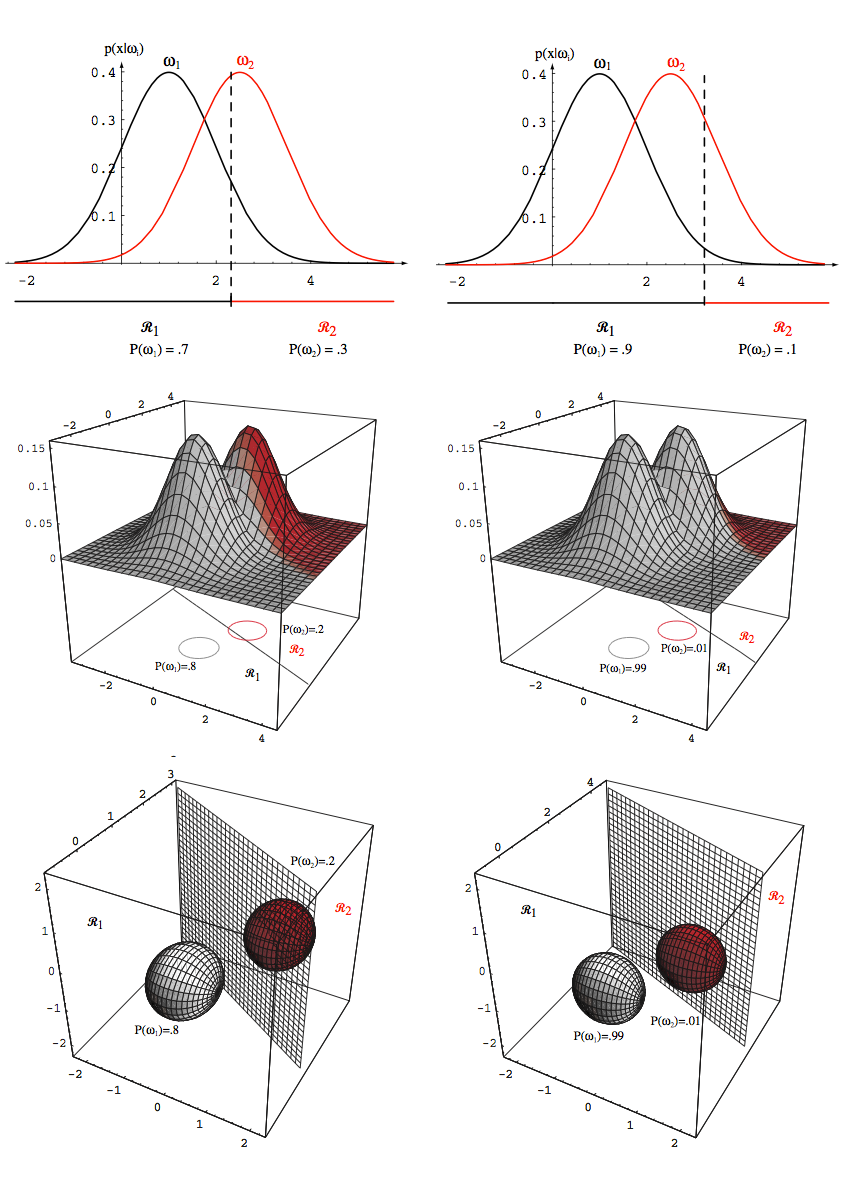
\includegraphics[scale=0.55]{img/hyperpiano.png}
\caption{Quando le probabilità a priori cambiano, la regione di decisione shifta}
\label{fig_iperpiano}
\end{figure}
Se $P(\omega_i) \neq P(\omega_j)$, il punto $\mathbf{x}_0$ si muove fra le due medie. Se invece le probabilità a priori $P(\omega_i)$ sono uguali per tutte le $c$ classi, allora anche il termine $\ln P(\omega_i)$ può essere ignorato. Per classificare un vettore delle caratteristiche $\mathbf{x}$, si misura la distanza euclidea $\norma{\mathbf{x} - \mu_i}$ da ogni vettore delle medie $\mu_i$ delle $c$ classi e viene assegnato $\mathbf{x}$ alla classe più vicina. Per questo motivo è anche detto \emph{classificatore a minima distanza}. 

\subsection{Caso 2: $\mathbf{\Sigma}_i = \mathbf{\Sigma}$}
Un altro semplice caso è quando le matrici di covarianza per tutte le classi sono uguali. Geometricamente corrisponde alla situazione in cui la sezione della gaussiana vista dall'alto corrisponde ad un ellissoide, tutte della stessa diemensione e forma, ognuna centrata nel vettore delle medie $\mu_i$. Anche in questo caso sia $\abs{\mathbf{\Sigma}_i}$ che $(d/2) \ln 2\pi$ nell'equazione \ref{fun} non dipendono dalle classi e quindi possono essere ignorati, come prima la semplificazione porta alla seguente funzione discriminante
\begin{equation}
g_i(\mathbf{x})  =\frac{1}{2}(\mathbf{x} - \mu_i)' \mathbf{\Sigma}^{-1}(\mathbf{x} - \mu_i) + \ln P(\omega_i)
\end{equation}
come si può osservare anche in questo caso il classificatore è lineare, quindi è un hyperpiano.
Se le probabilità a priori $P(\omega_i)$ sono uguali per tutte le $c$ classi, allora anche in questo caso il temine $\ln P(\omega_i)$ può essere ignorato. Anche in questo caso la regola di decisione risulta essere davvero semplice: Per classificare il vettore $\mathbf{x}$ si calcola la distanza di \emph{Mahalanobis} $(\mathbf{x} - \mu_i)' \mathbf{\Sigma}^{-1}(\mathbf{x}- \mu_i)$ da ogni vettore delle medie, e si assegna $\mathbf{x}$ a quello più vicino. Come prima se ci si trova di fronte a probabilità a priori diverse per ogni classe allora queste condizionano la decisione verso la categoria che ha pobabilità più alta. 

\subsection{Caso 3: $\mathbf{\Sigma}_i$ = arbitrario}
Nel caso generale di una distribuzione normale multivariata, allora le matrici di covarianza sono diverse per ogni classe. L'unico termine che può essere ignorato è $(d/2) \ln 2\pi$ e la funzione discriminante risulta essere una quadrica. Ovvero una forma qualsiasi che rappresenta esattamente un classificatore chiamato quadratico, in tal caso le superfici di decisione non sono iperpiani ma sono delle iperquadriche, paraboloidi che si intersecano. 

\section{Probabilità di errore ed integrali}
Consideriamo prima il caso a due categoria e supponiamo che il classificatore abbia separato le due regioni $\mathcal{R}_1$ e $\mathcal{R}_2$. Ci sono due modi nel quale il classificatore può commettere un errore: quello di assegnare l'osservazione $\mathbf{x}$ alla regione $\mathcal{R}_2$ quando il suo vero stato della natura doveva essere $\omega_1$ e quello di assegnare l'osservazione $\mathbf{x}$ alla regione $\mathcal{R}_1$ quando il suo vero stato della natura doveva essere $\omega_2$. Poichè questi eventi sono mutuamente esclusivi allora la probabilità di errore è calcolata come segue
\begin{equation}
\begin{split}
P(error) &= P(\mathbf{x} \in \mathcal{R}_2, \omega_1) + P(\mathbf{x} \in \mathcal{R}_1, \omega_2) \\
&= P(\mathbf{x} \in \mathcal{R}_2|\omega_1) P(\omega_1) + P(\mathbf{x} \in \mathcal{R}_1|\omega_2) P(\omega_2)\\
&= \int_{\mathcal{R}_2} p(\mathbf{x}|\omega_1) P(\omega_1) \ d\mathbf{x} + \int_{\mathcal{R}_1} p(\mathbf{x}|\omega_2) P(\omega_2) \ d\mathbf{x}
\end{split}
\end{equation}

\noindent Il risultato nel caso monodimensionale è illustrato in figura \ref{errore}. I due integrali calcolati sono rappresentati dall'area rosa e grigia. Dato che il punto di decisione è $x^*$ la probabilità di errore non è minima. In particolare l'aria marcata con il bordo rosso è l'errore riducibile che può essere ridotto spostando il punto di decisione verso $x_B$. Nel caso multicategoria, invece è più semplice calcolare la probabilità di correttezza nel modo seguente
\begin{equation}
\begin{split}
P(correct) &= P(\mathbf{x} \in \mathcal{R}_i, \omega_i) \\
&= \sum_{i=1}^c P(\mathbf{x} \in \mathcal{R}_i | \omega_i) P(\omega_i) \\
&= \sum_{i=1}^c \int_{\mathcal{R}_i} p(\mathbf{x}|\omega_i)P(\omega_i) \ d\mathbf{x}
\end{split}
\end{equation} 
In questo caso si fa uso della sommatoria perchè le classi sono $c$, quindi un insieme finito e numerabile, quindi la probabiità di appartenenza di ogni classe è discreta, invece è continua la densità di probabilità. 


\begin{figure}
\centering
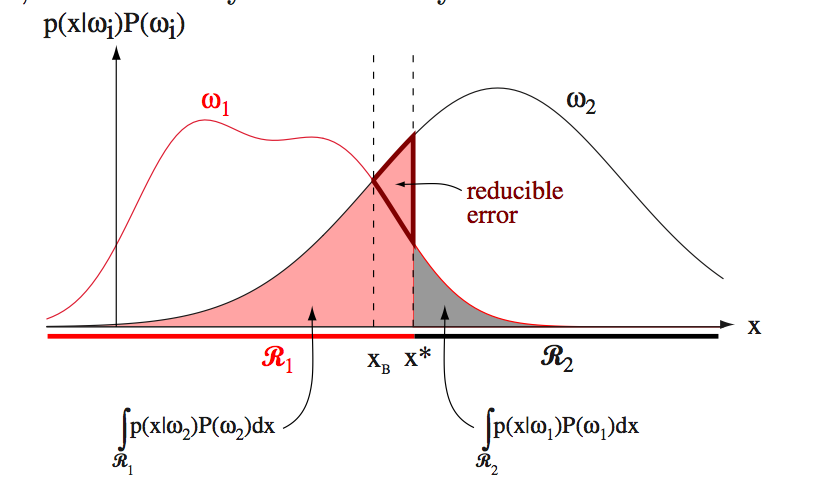
\includegraphics[scale=0.45]{img/errore.png}
\caption{Probabilità di errore nel caso il punto di decisione sia $x^*$. L'area rosa corrisponde alla probabilità di errore di decidere lo stato $\omega_1$ quando dovrebbe essere $\omega_2$; l'area grigia corrisponde alla situazione opposta.}
\label{errore}
\end{figure}

\subsection{Receiver Operating Characteristic (R.O.C.)}
Osservando al figura \ref{errore1} possiamo distinguere quattro aree
\begin{itemize}
\item $P(x > x^* | x \in \omega_2)$: La probabilità che l'osservazione venga classificata come $\omega_2$ e appartiene alla classe $\omega_2$, quindi una classificazione esatta che viene indicata in genere con i seguenti termini: \emph{hit} o \emph{true positive}
\item $P(x > x^* | x \in \omega_1)$:  La probabilità che l'osservazione venga classificata come $\omega_2$ e appartiene alla classe $\omega_1$, quindi una classificazione non corretta che viene indicata in genere con i seguenti termini: \emph{false alarm} o \emph{false positive} 
\item $P(x < x^* | x \in \omega_2)$:  La probabilità che l'osservazione venga classificata come $\omega_1$ e appartiene alla classe $\omega_2$, quindi una classificazione non corretta che viene indicata in genere con i seguenti termini: \emph{miss} o \emph{false negative}
\item $P(x < x^* | x \in \omega_1)$:  La probabilità che l'osservazione venga classificata come $\omega_1$ e appartiene alla classe $\omega_1$, quindi una classificazione corretta che viene indicata in genere con i seguenti termini: \emph{correct rejection} o \emph{true negative}
\end{itemize}
\begin{figure}
\centering
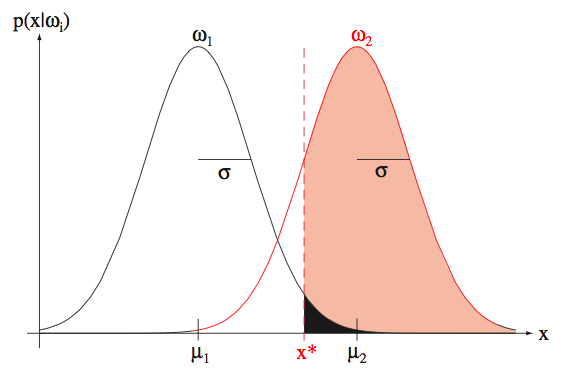
\includegraphics[scale=0.5]{img/errore1.png}
\caption{}
\label{errore1}
\end{figure}
Le curve di ROC è un plot che si basa sui valori ottenuti dalla matrice di confusione, quindi in un primo passo si calcola la matrice di confusione.
\[
\left(
\begin{array}{cc}
 VP & FP \\
 FN & VN 
\end{array}
\right)
\]
ROC sta per \emph{Receiver Operating Characteristic}, sostanzialmente ci aspettiamo che questo sistema segnali correttamente o non correttamente e vogliamo misurare il comportamento, cioè la rilevazione di un oggetto oppure il verificarsi di un evento. La ROC (Fig. \ref{roc}) è una curva che viene plottata nello spazio bidimensionale, sull'asse delle ascisse viene riportato il \emph{false positive rate} oppure più comunemente la Specificità, cioè il rapporto dei casi classificati come corretti ma appartenenti ad una classe diversa \emph{false positive}, rispetto al numero totale dei casi negativi, quindi
\begin{equation}
S_p = \frac{FP}{FP+VN}
\end{equation}
invece sull'asse delle ordinate abbiamo il \emph{true positive rate}, oppure più comunemente la Sensibilità cioè il rapporto dei casi positivi classificati come positivi ed il numero totale dei casi positivi, quindi
\begin{equation}
S_e = \frac{VP}{VP+FN}
\end{equation}
Il risultato desiderato è quello che il classificatore ci desse il  massimo per il \emph{true positive rate} (sensibilità) mentre il \emph{false positive rate} (specificità) sia minimo, quindi ci si aspetta il grafico mostrato in figura \ref{roc}.
\begin{figure}
\centering
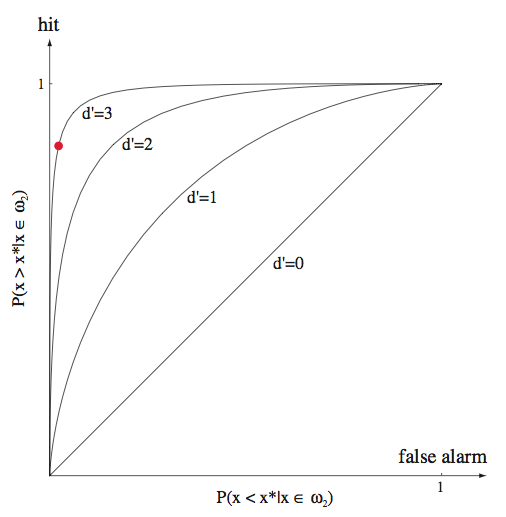
\includegraphics[scale=0.5]{img/roc.png}
\caption{}
\label{roc}
\end{figure}
L’analisi ROC viene effettuata attraverso lo studio della funzione che  lega la probabilità di ottenere un risultato vero-positivo nella classe dei pattern da classificare come veri (ossia la sensibilità) alla probabilità di ottenere un risultato falso-positivo nella classe dei pattern da classificare come falsi(ossia specificità). In altre parole, vengono studiati i rapporti fra allarmi veri (hit rate) e falsi allarmi. La capacità discriminante di un test, ossia la sua attitudine a separare propriamente la popolazione in studio è proporzionale all’estensione dell’area sottesa alla curva ROC (Area Under Curve, AUC). Nel caso di un test perfetto, ossia che non restituisce alcun falso positivo né falso negativo (capacità discriminante = $100\%$), la AUC passa attraverso le coordinate {0;1} ed il suo valore corrisponde all’area dell’intero quadrato delimitato dai punti di coordinate (0,0), (0,1), (1,0) (1,1), che assume valore 1 corrispondendo ad una probabilità del $100\%$ di una corretta classificazione. 


%%%%%%%%%%%%%%%%%%%%% chapter.tex %%%%%%%%%%%%%%%%%%%%%%%%%%%%%%%%%
%
% sample chapter
%
% Use this file as a template for your own input.
%
%%%%%%%%%%%%%%%%%%%%%%%% Springer-Verlag %%%%%%%%%%%%%%%%%%%%%%%%%%

\chapter{Maximum-Likelihood and Bayesian Parameter Estimation}\label{tecnicheParametriche}
\section{Introduzione}
Nella sezione \ref{teoriaBaesiana} abbiamo visto come progettare un classificatore conoscendo le probabilità a priori $P(\omega_i)$ e le funzioni di distribuzione di probabilità condizionate $p(\mathbf{x}|\omega_i)$. Sfortunatamente, nei problemi di pattern recgnition non sempre abbiamo una conoscenza completa della struttura probabilistica. Nel caso tipico abbiamo una vaga conoscenza della situazione insieme al numero dei dati di \emph{training}. Il problema è quindi quello progettare un classificatore usando queste informazioni.  Supponiamo per esempio che $p(\mathbf{x}|\omega_i)$ è una distribuzione normale con media $\mathbf{\mu_i}$ e matrice d covarianza $\mathbf{\Sigma_i}$, malgrado non conosciamo questi valori. Il problema può essere semplificato stimando soltanto i parametri $\mathbf{\mu_i}$ e $\mathbf{\Sigma_i}$ piuttosto che stimare la funzione di probabilità $p(\mathbf{x}|\omega_i)$.\\

\noindent La stima dei parametri è un classico problema statistico, è può essere affrontato in molti modi. Considereremo le comuni procedure chiamate rispettivamente \emph{maximum-likelihood estimation} (stima massima verosomiglianza) e \emph{Bayesian estimation} (stima Baiesiana).\\

\noindent \'E importante fare una distinzione tra i metodi di addestramento \emph{supervised} e \emph{unsupervised}. In entrambi i casi valgono le regole delle probabilità a priori e la verosomiglianza, si differiscono dal fatto che nel primo caso conosciamo lo stato della natura per ogni classe, quindi è possibile etichettare le classi, cosa che non conosciamo nell'addestramento \emph{unsupervised}, problema molto più difficile da affrontare. 

\section{Maximum-Likelihood Estimation} 
Supponiamo di avere $c$ Data sets $\mathcal{D}_1, \dots, \mathcal{D}_c$, dove ogni campione in $D_j$ viene descritto da una distribuzione $p(\mathbf{x}|\omega_j)$. Inoltre è necessario che i campioni siano \emph{i.i.d.}\footnote{Nella teoria della probabilità una sequenza di variabili casuali è \emph{i.i.d.} se ognuna ha la stessa distribuzione di probabilità delle altre variabili e sono tutte statisticamente indipendenti, cioè che il verificarsi di uno non cambia la probabilità di verificarsi dell'altro}, ovvero che le variabili casuali siano distribuite indipendentemente e identicamente. Assumiamo anche che $p(\mathbf{x}|\omega_j) \sim N(\mathbf{\mu_j, \Sigma_j})$, quindi descrivibile dai parametri $\mathbf{\mu_j \ \text{e} \ \Sigma_j}$ e che questi parametri vengono rappresentati dal vettore $\mathbf{\Theta_j}$. Il problema è quello di conoscere $\mathbf{\Theta_j}$, ovvero i parametri del modello, dato l'insieme dei dati.  L'idea è quella di trovare un un insieme di parametri $\mathbf{\Theta_j}$ che vanno sostituiti nella distribuzione di probabilità, l'obiettivo è quello di ottenere una distribuzione molto verosimile $p(\mathcal{D}|\mathbf{\Theta})$ (verosomiglianza) alla distribuzione dei dati originali. Supposto che $\mathcal{D}$ contiene $n$ campioni $\mathbf{x_1, \dots, x_n}$ allora $p(\mathcal{D}|\mathbf{\Theta}) = p(\mathbf{x_1, \dots, x_n}|\mathbf{\Theta})$, poichè abbiamo assunto che i campioni sono \emph{i.i.d} allora
\begin{equation}
p(\mathcal{D}|\mathbf{\Theta}) = \prod_{k=1}^n p(\mathbf{x_k}|\mathbf{\Theta})
\end{equation}
La stima della massima verosomiglianza, per definizione è il valore $\mathbf{\hat{\Theta}}$ che massimizza $p(\mathcal{D}| \mathbf{\Theta})$. Per semplicità analitica è preferibile lavorare con i logaritmi, in quanto il logaritmo di una produttoria diventa una sommatoria, quindi definiamo $l(\mathbf{\Theta})$ come la funzione \emph{log-likelihood}
\begin{equation}
l(\mathbf{\theta}) \equiv \ln p(\mathcal{D}|\mathbf{\Theta})
\end{equation}
quindi, come detto prima il logaritmo di una produttoria diventa la sommatoria dei logaritmi
\begin{equation}
l(\mathbf{\theta})  = \sum_{k=1}^n  \ln p(\mathbf{x_k|\Theta})
\end{equation}
l'obiettivo principale è quello di trovare $\mathbf{\Theta}$ che massimizza la funzione \emph{log-likelihood}, quindi
\begin{equation}
\mathbf{\hat{\Theta}} = \arg \max l(\mathbf{\Theta})
\end{equation}
Sappiamo che per trovare il massimo di una funzione si calcola la derivata prima e si pone uguale a zero, in questo caso il numero di parametri da stimare è $p$, quindi calcoliamo la derivata di una funzioni a più varabiali. Denotiamo $\mathbf{\Theta}$ come un vettore a $p-$componenti $\mathbf{\Theta} = (\Theta_1, \dots, \Theta_p)$ e con $\mathbf{\nabla_\Theta}$ denotiamo l'operatore gradiente
\begin{equation}\label{gradiente}
    \mathbf{\nabla_\Theta} =
    \begin{bmatrix}
    \frac{\partial}{\partial \Theta_1} \\
    \vdots \\
    \frac{\partial}{\partial \Theta_p}
    \end{bmatrix}
\end{equation}
la derivata di una sommatoria non è altro che la somma delle derivate, quindi
\begin{equation}\label{6}
\mathbf{\nabla_\Theta}l = \sum_{k=1}^n \mathbf{\nabla_\Theta} \ln p(\mathbf{x}_k| \mathbf{\Theta})
\end{equation}
per stimare la massima verosomiglianza (MLE) basta risolvere questo sistema di equazioni
\begin{equation}\label{7}
\mathbf{\nabla_\Theta}l = 0
\end{equation}
per ottenere la soluzione $\mathbf{\hat{\Theta}}$.\\

\noindent La massima verosomiglianza rappresenta il punto in cui il campione osservato è più probabilie, la procedura del gradiente può portare a trovare il massimo locale ma non il massimo assoluto, ciò significa che non si ha una soluzione ottima ma una soluzione subottima. Quindi bisogna considerare ogni soluzione individualmente per poi trovare l' ottimo globale, massimo dei massimi locali. 

\subsection{Caso Gaussiamo: $\mathbf{\mu}$ incognita }
Vediamo adesso come il metodo ML (maximum-likelihood) viene applicato ad uno specifico caso,  supponiamo che i campioni si distribuiscono secondo una distribuzione normale multivariata con media $\mathbf{\mu}$ e matrice di covarianza $\mathbf{\Sigma}$. Per semplicità, consideriamo il caso in cui soltanto la media è sconosciuta. Sotto questa condizione, consideriamo come campione il punto $\mathbf{x}_k$ e calcoliamo
\begin{equation}\label{63}
\ln p(\mathbf{x}_k|\mathbf{\mu}) = -\frac{1}{2} \ln \left[ (2\pi)^d \abs{\mathbf{\Sigma}} \right]  - \frac{1}{2}(\mathbf{x}_k - \mathbf{\mu})' \Sigma^{-1}(\mathbf{x}_k - \mathbf{\mu})
\end{equation}
dato che $p(\mathbf{x}_k|\mathbf{\mu}) \sim N(\mathbf{\mu_j, \Sigma_j})$ allora si dimostra che la \ref{63} è stata ricavata mediante semplici passaggi matematici applicati alla distribuzione gaussiana multvariata che ricordiamo essere
\begin{equation}\label{distribuzioneMultivariata}
p(\mathbf{x}_k|\mu) = \frac{1}{(2\pi)^{d/2} \abs{\mathbf{\Sigma}}^{1/2}} \exp \left [ - \frac{1}{2} (\mathbf{x}_k - \mathbf{\mu})'  \mathbf{\Sigma}^{-1} (\mathbf{x}_k - \mathbf{\mu}) \right ]
\end{equation}
abbiamo detto che lavoriamo con i logaritmi quindi diventa
\begin{equation}
\begin{split}
\ln p(\mathbf{x}_k|\mu) &= \ln \frac{1}{(2\pi)^{d/2} \abs{\mathbf{\Sigma}}^{1/2}} - \frac{1}{2} (\mathbf{x}_k - \mathbf{\mu})'  \mathbf{\Sigma}^{-1} (\mathbf{x}_k - \mathbf{\mu})\\
&= - \left( \ln (2\pi)^{d/2} \abs{\mathbf{\Sigma}}^{1/2} \right) - \frac{1}{2} (\mathbf{x}_k - \mathbf{\mu})'  \mathbf{\Sigma}^{-1} (\mathbf{x}_k - \mathbf{\mu})\\
&= - \left( \ln \left[ (2\pi)^d \abs{\mathbf{\Sigma}} \right]^{1/2} \right) - \frac{1}{2} (\mathbf{x}_k - \mathbf{\mu})'  \mathbf{\Sigma}^{-1} (\mathbf{x}_k - \mathbf{\mu})\\
&= - \frac{1}{2} \ln \left[ (2\pi)^d \abs{\mathbf{\Sigma}} \right] - \frac{1}{2} (\mathbf{x}_k - \mathbf{\mu})'  \mathbf{\Sigma}^{-1} (\mathbf{x}_k - \mathbf{\mu})
\end{split}
\end{equation}
deriviamo rispetto a $\mu$, quindi consideriamo costantela matrice di covarianza $\mathbf{\Sigma}$ ed otteniamo
\begin{equation}\label{9}
\mathbf{\nabla}_{\mu} \ \ln p(\mathbf{x}_k|\mathbf{\mu}) = \mathbf{\Sigma}^{-1} (\mathbf{x}_k - \mathbf{\mu})
\end{equation}
Identificando $\mathbf{\Theta}$ con $\mathbf{\mu}$, osserviamo che dalle equazioni \ref{6}, \ref{7} e \ref{9} la stima a massima verosomiglianza per la media $\mathbf{\mu}$ deve soddisfare 
\begin{equation}
\sum_{k=1}^n \mathbf{\Sigma}^{-1} (\mathbf{x}_k - \mathbf{\hat{\mu}}) = 0
\end{equation}
moltiplicando per $\mathbf{\Sigma}$ e riarrangiando, otteniamo
\begin{gather}
\sum_{k=1}^n (\mathbf{x}_k - \mathbf{\hat{\mu}}) = 0\\
\sum_{k=1}^n \mathbf{x}_k -  \sum_{k=1}^n \mathbf{\hat{\mu}} = 0\\
\sum_{k=1}^n \mathbf{x}_k  =  \sum_{k=1}^n \mathbf{\hat{\mu}}\\
\sum_{k=1}^n \mathbf{x}_k  =  n \mathbf{\hat{\mu}}\\
\end{gather}
da cui $\mu$ è uguale a 
\begin{equation}
\mathbf{\hat{\mu}} = \frac{1}{n}\sum_{k=1}^n \mathbf{x}_k
\end{equation}
Questo è un risultato soddisfacente. Vuol dire che per la stima a massima verosomiglianza di una distribuzione con media sconosciuta, la media è la semplice media aritmetica sui campioni di training. Geometricamente se pensiamo gli $n$ campioni come una nuvola di punti, la media non è altro che il centroide della nuvola.  

\subsection{Caso Gaussiano: $\mathbf{\mu}$ e $\mathbf{\Sigma}$ incognite }
Nel caso più generale ne la media $\mathbf{\mu}$ ne la matrice di covarianza $\mathbf{\Sigma}$ sono conosciuti. Questi due parametri costituiscono proprio i parametri del vettore $\mathbf{\Theta}$. Consideriamo prima il caso univariato con $\Theta_1 = \mu$ e $\Theta_2 =\sigma^2$. In questo caso la log-likelihood di un singolo campione è
\begin{equation}\label{74}
\ln p(x_k|\mathbf{\Theta}) = -\frac{1}{2}\ln 2\pi \Theta_2 - \frac{1}{2\Theta_2}(x_k-\Theta_1)^2
\end{equation}
questa volta, dato che stiamo affrontando il caso unidimensionale allora la \ref{74} è stata ottenuta applicando semplici passaggi matematici alla
\begin{equation}
p(x_k| \mathbf{\Theta}) = \frac{1}{\sqrt{2\pi} \sigma} \exp  \left [ -\frac{1}{2}  \left (  \frac{x - \mu}{\sigma} \right )^2 \right  ]
\end{equation}
come prima, per seplicità analitica applichiamo la funzione logaritmo, quindi
\begin{equation}
\begin{split}
\ln p(x_k| \mathbf{\Theta}) &= \ln \frac{1}{\sqrt{2\pi \sigma^2}} -\frac{1}{2}  \left (  \frac{x - \mu}{\sigma} \right )^2\\
&= - \ln \sqrt{2\pi \sigma^2} -\frac{1}{2}  \left (  \frac{x - \mu}{\sigma} \right )^2\\
&= - \frac{1}{2} \ln2 \pi \sigma^2 -\frac{1}{2\sigma^2}  \left ( x - \mu \right )^2
\end{split}
\end{equation}
sostituendo $\Theta_1 = \mu$ e $\Theta_2 =\sigma^2$ otteniamo proprio la \ref{74}
\begin{equation}\label{77}
\ln p(x_k|\mathbf{\Theta}) = -\frac{1}{2}\ln 2\pi \Theta_2 - \frac{1}{2\Theta_2}(x_k-\Theta_1)^2
\end{equation}
adesso andiamo a derivare rispetto a $\Theta_1$ e $\Theta_2$ calcolando le seguenti derivate parziali $\frac{\partial }{ \partial \Theta_1}$ e $\frac{\partial }{ \partial \Theta_2}$. Cominciamo con la $\frac{\partial }{ \partial \Theta_1}$ e quindi subito osserviamo che risulta costante dato che consideriamo $\Theta_2$ costante, quindi la sua derivata è zero. Procediamo col derivare soltanto il secondo membro ottenendo così
\begin{equation}
\frac{\partial }{ \partial \Theta_1} = \frac{1}{\Theta_2}(x_k - \Theta_1) 
\end{equation}
i passaggi per calcolare la $\frac{\partial }{ \partial \Theta_2}$ risultano leggermente lunghi e quindi è opportuno fare anche un richiamo di alcune regole di derivazione come la derivata del prodotto di due funzioni, il rapporto di due funzioni ed il logaritmo di una funzione
\begin{gather}
\frac{\partial}{\partial x}(f(x)\cdot g(x)) = f'(x)\cdot (x) + f(x) \cdot g'(x)\\
\frac{\partial}{\partial x} \left( \frac{f(x)}{g(x)} \right) = \frac{f'(x)\cdot (x) + f(x) \cdot g'(x)}{[g(x)]^2}\\
\frac{\partial}{\partial x} \log(g(x)) = \frac{1}{g(x)} \cdot g'(x)
\end{gather}
quindi richiamate queste seguenti regole possiamo procedere con il calcolo di $\frac{\partial }{ \partial \Theta_2}$. Prendiamo il primo membro della \ref{77} e lo deriviamo rispetto a $\Theta_1$
applicando le regole di derivazione viste sopra, applichiamo quella del prodotto e quella del logaritmo ottenendo cosi $- \frac{1}{2 \pi \Theta_2} 2\pi$, semplifichiamo ed otteniamo la derivata del primo membro $-\frac{1}{2 \Theta_2}$. Per il secondo membro della \ref{77} applichiamo la regola del prodotto ponendo $f(x) = \frac{1}{2\Theta_2}$ e $g(x) = (x_k-\Theta_1)^2$ per calcolare $f'(x)$ utilizziamo la regola del rapporto, quindi $-\frac{2}{4 \Theta_2^2}$, semplificando $-\frac{1}{2 \Theta_2^2}$ che moltiplichiamo per $g(x)$ ottenendo $-\frac{1}{2 \Theta_2^2} (x_k-\Theta_1)^2$, la seconda parte della regola del prodotto è pari a zero dato che $g'(x) = 0$.  Riscrivendo i risultati ottenuti abbiamo che
\begin{equation}
\frac{\partial }{ \partial \Theta_2} =  -\frac{1}{2 \Theta_2} + \frac{1}{2 \Theta_2^2} (x_k-\Theta_1)^2
\end{equation}
quindi, calcolare le derivate parziale costruiamo il vettore gradiente
\begin{equation}
\mathbf{\nabla}_\Theta l = \mathbf{\nabla}_\Theta \ln p(x_k|\mathbf{\Theta}) =
    \begin{bmatrix}
    \frac{1}{\Theta_2}(x_k - \Theta_1) \\
    \\
    -\frac{1}{2 \Theta_2} + \frac{(x_k - \Theta_1)^2}{2 \Theta_2^2}
    \end{bmatrix}
\end{equation}
abbiamo detto che la derivata di una sommatoria non è altro che la somma delle derivate, poniamo le derivate uguali a zero e risolviamo
\begin{equation}
\sum_{k=1}^n \frac{1}{\hat{\Theta}_2}(x_k -\hat{\Theta}_1) = 0
\end{equation}
e
\begin{equation}
- \sum_{k=1}^n \frac{1}{2 \hat{\Theta}_2} + \sum_{k=1}^n \frac{(x_k - \hat{\Theta}_1)}{2 \hat{\Theta}_2^2} = 0
\end{equation}
dove $\hat{\Theta}_1$ e $\hat{\Theta}_2$ sono i valori che massimizzano la stima di probabilità. Sostituendo $\hat{\mu} = \hat{\Theta}_1$ e $\sigma^2 = \hat{\Theta}_2$ e facendo gli opportuni riarrangiamenti otteniamo che 
\begin{equation}
\hat{\mu} = \frac{1}{n} \sum_{k=1}^n x_k
\end{equation}
e
\begin{equation}
\hat{\sigma}^2 = \frac{1}{n} \sum_{k=1}^n (x_k- \hat{\mu})^2
\end{equation}
Nel caso multivariato è tutto molto simile la stima a massima verosomiglianza per i parametri $\mu$ e $\mathbf{\Sigma}$ è calcolata mediante le seguenti formule
\begin{equation}
\hat{\mu} = \frac{1}{n} \sum_{k=1}^n \mathbf{x_k}
\end{equation}
e
\begin{equation}
\hat{\mathbf{\Sigma}} = \frac{1}{n} \sum_{k=1}^n (\mathbf{x}_k - \hat{\mu})(\mathbf{x}_k - \hat{\mu})'
\end{equation}
Ancora una volta osserviamo che la stima del vettore delle medie è semplicemente la media mentre la stima per la matrice di covarianza è la media aritmetica delle $n$ matrici $(\mathbf{x}_k - \hat{\mu})(\mathbf{x}_k - \hat{\mu})'$. 

\section{Bayesian Estimation (cenni)} 
L'idea è quella aumentare di volta in volta il numero di campioni ed ad ogni passo calcolare media e varianza (o matrice di covarianza). Dopodiché viene effettuata una media delle medie e una media delle varianze per stimare i parametri.

\section{Principal Component Analysis}
La PCA è una tecnica utile per la comprensione e la classificazione dei dati. Lo scopo è quello di ridurre la dimensionalità dei dati (quindi la dimensione dei pattern di ogni campione e non il numero di campioni)  trovando un insieme nuovo di variabili, in numero ridotto rispetto alle dimensioni dell'insieme originale di variabili, che trattengono comunque la maggior parte delle informazioni originali dei dati iniziali. Per informazione intendiamo la variazione presente nel campione, per esempio se non c'è variazione nei dati allora non daranno nessuna informazione in quanto sarebbero tutti uguali. Quindi informazione è uguale a variazione e variazione è uguale a varianza o a matrice di covarianza. In generale questa variazione è rappresentata dalle correlazioni tra variabili originali. Ipotizziamo di avere delle variabili casuali, ricordiamo che il pattern $\mathbf{x}$ è sempre un vettore di variabili casuali, allora se prendo due vettori $\mathbf{x}_1$ e $\mathbf{x}_2$ di cinque componenti ognuno, e le cinque componenti sono pressoché uguali allora uno dei due si può buttar via. Analogamente se ho cento vettori, tutti con le stesse componenti allora ne prendo uno e quindi gli altri novantanove è inutile prenderli in considerazione dato che non danno alcuna informazione. In realtà considero solo quelli che variano sostanzialmente, quindi c'è una buona varianza sulle componenti. Se ho un vettore a $d$ dimensioni, quindi ho $d$ variabili casuali, l'idea è quella di trasformare questi pattern in altri pattern, quindi effettuare una trasformazione di spazio da uno spazio a $d$ dimensioni ad uno spazio a $k$ dimensioni, dove ovviamente $k < d$, da precisare che non si effettua una selezione, quindi non vengono prese in considerazione soltanto $k$ delle $d$ componenti ma viene effettuata un analisi e quindi un cambiamento delle variabili. Delle nuove variabili nessuna è uguale a quelle precedenti, ma sono tutte e $k$ nuove. Queste variabili vanno determinate in virtù di un criterio, cioè quello di conservare la maggiore informazione possibile delle $d$ componenti, sostanzialmente e necessario trattenere quelle che hanno maggiore varianza.\\

\noindent Facciamo un esempio, osservando la figura \ref{pca}.
\begin{figure}
\centering
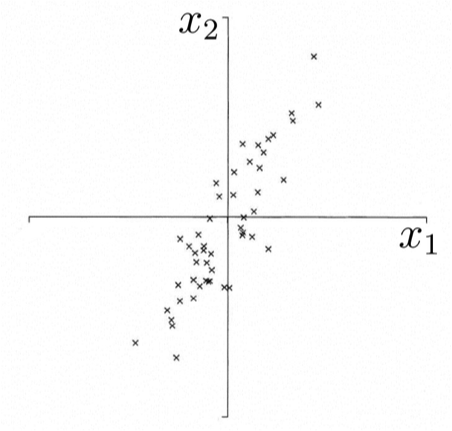
\includegraphics[scale=0.8]{img/pca.png}
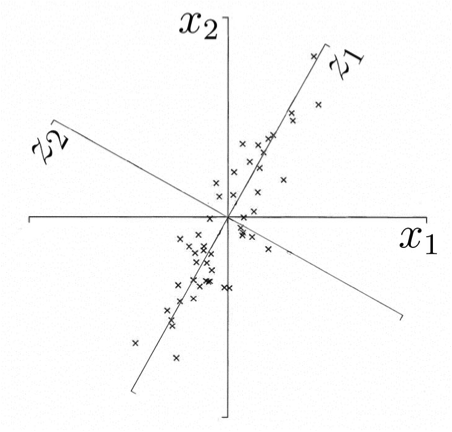
\includegraphics[scale=0.8]{img/pca1.png}
\label{pca}
\end{figure}
Immaginiamo di avere questi dati disposti in uno spazio bidimensionale (la PCA non si applica mai ad uno spazio bidimensionale in quanto non c'è nulla da ridurre). I dati sono disposti in modo tale che ci sia una varianza, inoltre questi dati potrebbero essere raggruppati in un cluster che potrebbe essere un ellisse. Supponiamo di sapere che questi dati appartengono a due cluster differenti. Allora qual'è il principio utilizzato per dividere questi dati? Esempio un metodo potrebbe essere quello di classificare tutti i pattern che rientrano nel primo quadrante e così via, quindi una classificazione che sta avvenendo sulla densità ovvero sulla distribuzione. Fondamentalmente questa suddivisione sta avvenendo in base alla varianza, questo si può spiegare perchè per i dati che si trovano intorno all'origine, soprattutto in prossimità della bisettrice tra il secondo e quarto quadrante, la varianza è molto piccola, mentre per gli altri, quelli che si trovano sulla bisettrice tra il primo ed il terzo quadrante la varianza più grande, quindi danno molta più informazione rispetto agli altri. Allora fatte queste osservazioni, quale potrebbe essere la trasformazione di un dataset in un altro dataset? Cioè l'operazione di proiettare tutti i vettori in un altro spazio, in questo caso nello spazio delle bisettrici, oppure equivalentemente nello spazio degli autovettori della matrice di covarianza dei dati. La matrice di covarianza ha sulla diagonale principale le varianze e al di fuori della diagonale principale ha le covarianze ovvero le correlazioni tra coppie di componenti. Sostanzialmente stiamo dicendo che se andiamo a vedere la matrice di covarianza (in questo caso è una matrice $2\times2$) osserviamo che sulla diagonale principale abbiamo la varianza sulla prima componente e sulla seconda componente, ci aspettiamo che una delle due sia maggiore dell'altra. 
Si tende a proiettare i pattern sulle due bisettrici, o equivalentemente gli autovettori della matrice di covarianza che corrispondono proprio ai due assi. Se riuscissi a proiettare, dopo aver calcolato gli autovettori della matrice di covarianza, alla fine identifico come componente  principale $z_1$, cioè quella a varianza maggiore, mentre come seconda componente principale prendo in considerazione $z_2$, cioè quella in cui la varianza tra le due è minore. Inoltre si conosce che le varianze della matrice di covarianza sono direttamente proporzionali agli autovalori della matrice di covarianza, quindi autovalori o varianze piò meno sono la stessa cosa. A questo punto il giochino facile è quello di prendere i dati, fare la matrice di covarianza, calcolare gli autovettori e gli autovalori, ordinare in ordine decrescente gli autovalori e corrispondentemente gli autovettori, scegliere gli autovalori maggiori e  ci si ferma quando la somma di questi autovalori supera una certa soglia. \'E ovvio che la somma degli autovalori non può essere maggiore di uno, di conseguenza se ipotizziamo di volere l'$80\%$ d'informazione allora sulla somma totale degli autovalori devo prendere tanti autovalori che sommati non superano 0.8. Così mi scelgo $k$ componenti principali tale che $\sum_{i=1}^k \lambda_i \leq 0.8$. Dove $k$ rappresenta il numero di componenti principali che seleziono in corrispondenza di questi autovalori, quindi ho $k$ autovettori che sono i nuovi assi del nuovo spazio sul quale vado a proiettare i pattern. I pattern erano in $d$ dimensioni e adesso sono proiettati su $k$ dimensioni per cui i pattern divetano $k$ dimensionali. Qual'è il vantaggio? se io ho pattern a cento dimensioni e scopro che la maggiore informazione è concentrata nelle prime dieci componenti principali allora ho ridotto lo spazio da cento dimensioni in pattern di dimensione dieci, conservando l'$80\%$ dell'informazione. Tutto ciò ha una base teorica:\\

\noindent Preso un pattern di $p$ variabili $\mathbf{x} = \{x_1, \dots, x_p\}$ vogliamo calcolare la prima componente principale dell'insieme dei campioni come trasformazione lineare di $\mathbf{x}$ tale che $z_1$ abbia la maggiore informazione (o che la varianza sia massima), quindi possiamo scrivere
\begin{equation}\label{70}
z_1 = \mathbf{a}_1^T \mathbf{x} = \sum_{i=1}^p \mathbf{a}_{i1} x_i
\end{equation}
dove il vettore $\mathbf{a}_1 = \{ a_{11}, a_{21}, \dots, a_{p1}\}$, è il vettore di pesi. 
Questo è un problema di ottimizzazione, perchè ancora una volta lo scopo principale è quello di massimizzare. Di conseguenza se voglio trovare la $k$-esima componente principale allora la \ref{70} diventa
\begin{equation}
z_k = \mathbf{a}_k^T \mathbf{x} \quad \quad \quad k=1, \dots, p
\end{equation}
dove il vettore $\mathbf{a}_k = \{ a_{1k}, a_{2k}, \dots, a_{pk} \}$, come prima è il vettore dei pesi.
Naturalmente le componenti principali calcolate devono essere relative alle componenti principali precedenti. Quindi non solo vogliamo che la varianza di $z_k$ sia massima, ma vogliamo anche che la covarianza di $z_k$ e $z_l$ con $1 \leq l < k$ sia uguale a zero, cioè fondamentalmente che non ci sia correlazione. Oltre alle componenti principali in senso di massimizzare la varianza, un altro vincolo è quello di avere componenti scorrelate fra di loro. Un ulteriore condizione è che $\mathbf{a}_k^T \mathbf{a}_k  =1 $. Adesso vediamo come trovare la prima componente principale. La varianza di $z_1$ la possiamo anche scrivere mediante una forma altrenativa, cioè
\begin{equation}\label{72}
var(z_1) = E[z_1^2] - E[z_2]^2
\end{equation}
dove $E$ sta ad indicare la media. Dalla \ref{70} sappiamo che $z_1 = \mathbf{a}_1^T \mathbf{x}$, quindi $x_1^2$ equivale a moltiplicare
\begin{equation}
\begin{split}
z_1^2 &= \mathbf{a}_1^T\mathbf{x} \cdot \mathbf{a}_1^T\mathbf{x}\\
&= \sum_{i=1}^p \mathbf{a}_{i1} x_i \sum_{j=1}^p \mathbf{a}_{j1} x_j\\
&= \sum_{i,j=1}^p \mathbf{a}_{i1} \mathbf{a}_{j1} \mathbf{x}_i \mathbf{x}_j\\
\end{split}
\end{equation}
dato che stiamo calcolando la media di $z_1^2$ possiamo scrivere che
\begin{equation}
E[z_1^2] = \sum_{i,j=1}^p \mathbf{a}_{i1} \mathbf{a}_{j1} E[\mathbf{x}_i \mathbf{x}_j]
\end{equation}
Facciamo la stessa cosa per $E[z_2]^2$, ma questa volta calcoliamo il quadrato della madia quindi facendo le opportune moltiplicazioni otteniamo
\begin{equation}
\sum_{i,j=1}^p \mathbf{a}_{i1} \mathbf{a}_{j1} E[\mathbf{x}_i] E[\mathbf{x}_j]
\end{equation}
andando a sostituire nella \ref{72} i valori ottenuti per $E[z_1^2]$ e $[z_1]^2$ otteniamo
\begin{equation}
var(z_1) = \sum_{i,j=1}^p \mathbf{a}_{i1} \mathbf{a}_{j1} E[\mathbf{x}_i \mathbf{x}_j] - \sum_{i,j=1}^p \mathbf{a}_{i1} \mathbf{a}_{j1} E[\mathbf{x}_i] E[\mathbf{x}_j]
\end{equation}
a questo punto metto in evidenza la doppia sommatoria
\begin{equation}\label{76}
\sum_{i,j=1}^p \mathbf{a}_{i1} \mathbf{a}_{j1} \mathbf{S}_{ij} 
\end{equation}
dove $\mathbf{S}_{ij} = \sigma_{x_i,x_j}= E[\mathbf{x}_i \mathbf{x}_j] - E[\mathbf{x}_i] E[\mathbf{x}_j]$, $\mathbf{S}$ è la matrice di covarianza, quindi $\mathbf{S}_{ij}$ è l'elemento della matrice di covarianza. 
La \ref{76} può essere scritta come 
\begin{equation}
var(z_1) = \mathbf{a}_1^T \mathbf{S}\mathbf{a}_1
\end{equation}
A questo punto il problema è quello di massimizzare la varianza di $z_1$, quindi bisogna massimizzare  $var(z_1) = \mathbf{a}_1^T \mathbf{S}\mathbf{a}_1$ soggetto a $\mathbf{a}_1^T \mathbf{a}_1  = 1$. In questo caso si utilizza la teoria della regolarizzazione, fondamentalmente si utilizza il moltiplicatore di lagrange che porta il vincolo nella funzione obiettivo. In questo caso, dato che ho il vincolo $\mathbf{a}_1^T \mathbf{a}_1  = 1$ allora voglio che $\mathbf{a}_1^T \mathbf{a}_1  -1= 0$, data questa condizione allora è ovvio che $\mathbf{a}_1^T \mathbf{a}_1$ deve essere uguale ad uno. A questo punto devo massimizzare la funzione obiettivo che è  $\mathbf{a}_1^T \mathbf{S}\mathbf{a}_1$ più il vincolo,  ma poichè sto massimizzando allora devo massimizzare $-\mathbf{a}_1^T \mathbf{a}_1$, quindi
\begin{equation}
\mathbf{a}_1^T \mathbf{S}\mathbf{a}_1 + ( - \mathbf{a}_1^T \mathbf{a}_1  - 1)
\end{equation}
alla fine mi viene 
\begin{equation}
\mathbf{a}_1^T \mathbf{S}\mathbf{a}_1 - \mathbf{a}_1^T \mathbf{a}_1  -1 
\end{equation}
ovviamente la prima  parte è la funzione obiettivo originale, mentre la seconda parte è il vincolo che sto aggiungendo, a cui devo dare un peso $\lambda$ che prende il nome di moltiplicatore di lagrange
\begin{equation}
 \mathbf{a}_1^T \mathbf{S}\mathbf{a}_1 - \lambda(\mathbf{a}_1^T \mathbf{a}_1  -1)
\end{equation}
con $0 < \lambda \leq 1$. A questo punto è facile, come si trova il massimo di una funzione? derivata prima uguale a zero. Qual'è il valore per cui voglio ottenere il massimo? \'E $\mathbf{a}_1$. Perchè $\lambda$ lo fisso, $\mathbf{S}$ è la matrice di covarianza dei dati, quindi faccio la derivata rispetto ad $\mathbf{a}_1$, quindi pongo tutto uguale a zero
\begin{equation}
\mathbf{S}\mathbf{a}_1 - \lambda \mathbf{a}_1 = 0
\end{equation}
metto in evidenza $\mathbf{a}_1$
\begin{equation}
(\mathbf{S}-\lambda \mathbf{I}_p)\mathbf{a_1} = 0
\end{equation}
in questa equazione $\lambda$ è l'autovalore della matrice di covarianza e $\mathbf{a}_1$ non è altro che l'autovettore corrispondente.\\

\noindent Fin qui abbiamo massimizzato la varianza sulla prima componente principale, quindi $\lambda$ corrisponde all'autovalore maggiore, cioè sto massimizzando la varianza della prima componente principale, quindi fondamentalmente sto trovando la componente principale per la quale ho la massima varianza, massima varianza equivale a dire massimo autovalore. Quindi riassumendo, presi i dati, mi calcolo la matrice di covarianza $\mathbf{S}$, mi calcolo gli autovalori e gli autovettori della matrice di covarianza, il primo autovalore corrisponde alla massima varianza e l'autovettore corrispondente alla prima componente principale.\\
A questo punto ho calcolato $\mathbf{a}_1$ ma dalla \ref{70} dobbiamo ricavarci $z_1$ quindi moltiplicando $\mathbf{a}_1^T \mathbf{x}$ non faccio altro che la proiezione di $\mathbf{x}$ su $\mathbf{a}_1$ (il prodotto interno $\mathbf{a}_1^T \mathbf{x}$ non è altro che la proiezione di $\mathbf{x}$ su $\mathbf{a}_1$). \\
Quindi possiamo dire che la varianza della prima componente principale corrisponde all'autovalore maggiore. Dimostriamolo:
Traduciamo formalmente quello che abbiamo detto, quindi la varianza della prima componete è uguale al primo autovalore che corrisponde a quello maggiore
\begin{equation}\label{104}
var(z_1) = \lambda_1
\end{equation}
quindi dall'equazione
\begin{equation}
(\mathbf{S}-\lambda \mathbf{I}_p)\mathbf{a_1} = 0
\end{equation}
effettuando alcuni semplici passaggi matematici
\begin{equation}
\begin{split}
\mathbf{S}\mathbf{a}_1 - \lambda \mathbf{a}_1 &= 0 \\
\mathbf{S}\mathbf{a}_1 &=  \lambda \mathbf{a}_1\\ 
\mathbf{a}_1^T  \cdot \mathbf{S}\mathbf{a}_1 &=  \lambda \mathbf{a}_1 \cdot \mathbf{a}_1^T\\
\mathbf{a}_1^T\mathbf{S}\mathbf{a}_1 &=  \lambda \mathbf{a}_1^T\mathbf{a}_1\\
\mathbf{a}_1^T\mathbf{S}\mathbf{a}_1 &=  \lambda
\end{split}
\end{equation}
dato che $\mathbf{a}_1^T\mathbf{a}_1 =  1$ e $var(z1) = \mathbf{a}_1^T\mathbf{S}\mathbf{a}_1$, quindi è dimostrata la \ref{104}.\\


\noindent Ho trovato la prima componente principale corrispondente all' autovettore corrispondete all'autovalore maggiore cioè alla varianza maggiore, che in modo geometrico corrisponde alla proiezione di $\mathbf{x}$ sull'asse maggiore dell'ellissoide che circoscrive i dati.\\

\noindent La seconda componente principale come la calcolo? Massimizzando la varianza $z_2$ ma questa volta con il vincolo $\mathbf{a}_2^T\mathbf{a}_2 = 1$ quindi ho di nuovo 
\begin{equation}
 \mathbf{a}_2^T \mathbf{S}\mathbf{a}_2 - \lambda(\mathbf{a}_2^T \mathbf{a}_2  -1)
\end{equation}
solo che però voglio anche che la covarianza della seconda componente principale rispetto alla prima componente principale sia uguale a zero (che siano scorrelate). Allora si introduce un altro paramentro 
\begin{equation}
cov(z_2,z_1) = \mathbf{a}_1^T\mathbf{S}\mathbf{a}_2 = \lambda_1\mathbf{a}_1^T\mathbf{a}_2
\end{equation}
La $cov(z_2, z_1) = \mathbf{a}_1^T\mathbf{S}\mathbf{a}_2$ quindi fondamentalmente sarebbe l'elemento $S_{21}$ della matrice di covarianza, quindi la posso scrivere o come $\mathbf{a}_1^T\mathbf{S}\mathbf{a}_2$ oppure equivalentemente che lo possiamo scrivere anche come $\lambda_1\mathbf{a}_1^T\mathbf{a}_2$
questo si può dimostrare come precedentemente, 
\begin{equation}
\mathbf{S}\mathbf{a}_2 = \lambda_1 \mathbf{a}_2
\end{equation}
moltiplico entrambi i membri per $\mathbf{a}_1^T$ ed ottengo
\begin{equation}
\mathbf{a}_1^T \cdot \mathbf{S}\mathbf{a}_2 = \lambda_1 \mathbf{a}_2 \cdot \mathbf{a}_1^T
\end{equation}
ottenendo così
\begin{equation}
\mathbf{a}_1^T \mathbf{S}\mathbf{a}_2 = \lambda_1  \mathbf{a}_1^T \mathbf{a}_2 
\end{equation}
ma $\mathbf{a}_1^T \mathbf{S}\mathbf{a}_2$ non è altro che la $cov(z_2, z_1)$ per cui abbiamo dimostrato che
\begin{equation}
cov(z_2, z_1) = \lambda_1  \mathbf{a}_1^T \mathbf{a}_2 
\end{equation}
A questo punto dobbiamo minimizzare la covarianza che come prima significa massimizzare meno la covarianza. Quindi è necessario massimizzare $- \lambda_1  \mathbf{a}_1^T \mathbf{a}_2$. Facciamo la derivata rispetto ad $\mathbf{a_2}$ la poniamo uguale a zero e calcoliamo $\mathbf{a_2}$. Questo procedimento viene effettuato per $\mathbf{a_3}, \mathbf{a_4}, \dots, \mathbf{a_n}$ ottenendo tutte le altre componenti principale. In generale si può definire 
\begin{equation}
var(z_k) = \mathbf{a_k}^T \mathbf{S} \mathbf{a_k}
\end{equation}
che è uguale al k-esimo autovalore nell'ordine discendente, quindi dall'autovalore più grande all'autovalore più piccolo della matrice di covarianza. La k-esima componente principale trattiene la frazione maggiore della variazione del dataset dei campioni. 


%

%%%%%%%%%%%%%%%%%%%%% chapter.tex %%%%%%%%%%%%%%%%%%%%%%%%%%%%%%%%%
%
% sample chapter
%
% Use this file as a template for your own input.
%
%%%%%%%%%%%%%%%%%%%%%%%% Springer-Verlag %%%%%%%%%%%%%%%%%%%%%%%%%%

\chapter{Nonparametric Techniques}\label{metodinonparametrici}

\section{introduzione}
Nella sezione \ref{tecnicheParametriche} sono state trattate  le tecniche parametriche nel caso di addestramento \emph{supervised} assumendo una distribuzione di probabilità nota. Purtroppo nelle applicazioni di \emph{pattern recognition} non sempre abbiamo una conoscenza della distribuzione di probablità. In questa sezione verranno esaminate quelle tecniche chiamate \emph{nonparametric} che possono essere usate arbitrariamente con qualsiasi distribuzione senza assumere una conoscenza a priori. Ci sono molte tipologie di tecniche \emph{nonparametric}: in particolare una consiste nella procedura di stimare la funzione di densità $p(\mathbf{x}|\omega_j)$ dai campioni di \emph{patterns}, mentre un altra tecnica consiste invece in una procedura che stima direttamente la la probablità a posteriori $P(\omega_j|\mathbf{x})$.

\section{Stima della densità}
La probabilità $P$ che un vettore $\mathbf{x}$ ricade in una regione di decisione $\mathcal{R}$ è data da
\begin{equation}\label{P}
P = \int_{\mathcal{R}} p(\mathbf{x}') \ d\mathbf{x}'
\end{equation}
stiamo calcolando l'area che sottende la probabilità del campione $\mathbf{x}'$ all'interno della regione di decisione. $P$ è la versione media della funzione di densità $p(\mathbf{x})$, e possiamo stimare il valore di $p$ calcolando la probabilità $P$. Supponiamo di avere $n$ campioni $\mathbf{x}_1, \dots, \mathbf{x}_n$  che sono indipendenti e identicamente distribuiti (\emph{i.i.d.}) secondo la funzione di probabilità non nota $p(\mathbf{x})$. La probabilità che $k$ di questi $n$ campioni cada nella regione di decisione $\mathcal{R}$ è data dal coefficiente binomiale, ovvero la probabilità che $k$ degli $n$ campioni ricadano all'interno di una regione di decisione
\begin{equation}
P_k = \binom{n}{k} P^k (1-P)^{n-k}
\end{equation}
dove $P^k$ è la probabilità dei $k$ campioni che ricadono all'interno della regione $\mathcal{R}$, $(1-P)^{n-k}$ è la probabilità che $k$ campioni non ricadono all'interno della regione $\mathcal{R}$ e $\binom{n}{k}$ è il coefficiente binomiale, moltiplicando il tutto otteniamo $P_k$ che prende il nome di distribuzione binomiale. Inoltre il valore atteso di $k$ è
\begin{equation}
\varepsilon[k] = nP
\end{equation}
a questo punto vogliamo trovare quel parametro $k$ tale che abbiamo proprio la probabilità media, quindi se cambio il numero di campioni questa regola permane. Qual'è il valore per il quale ottengo esattamente $nP$? \'E proprio $k$. Con questa supposizione $k$ è approssimatiamente uguale ad $nP$, quindi essendo $k \simeq nP$, allora $P \simeq k/n$ sostituisco nella \ref{P} e di conseguenza otteniamo
\begin{equation}
\frac{k}{n} \simeq \int_{\mathcal{R}} p(\mathbf{x}') \ d\mathbf{x}'
\end{equation}
Individuata la regione di appartenenza dei punti, ipotizziamo di sceglierla piccola in modo tale da avere una densità della probabilità costante all'interno di essa, a questo punto la $p(\mathbf{x}')$ risulta essere costante rispetto ad $\mathbf{x}'$ e quindi è possibile portarla al di fuori dell'integrale e quindi il tutto diventa
\begin{equation}
\frac{k}{n} \simeq p(\mathbf{x}) \int_{\mathcal{R}} d\mathbf{x}'
\end{equation}
L'integrale $ \int_{\mathcal{R}} d\mathbf{x}'$ non è altro che un volume, quindi ho $p(\mathbf{x})V$, riprendendo la formula precedente 
\begin{equation}
\frac{k}{n} \simeq p(\mathbf{x})V
\end{equation}
riarrangiando viene fuori che una stima di $p(\mathbf{x})$ potrebbe essere
\begin{equation}\label{densita}
p(\mathbf{x}) = \frac{k/n}{V}
\end{equation}
dove $k$ è il numero di campioni che rientrano nella regione $\mathcal{R}$, $n$ è il numero di campioni in totale e $V$ è il volume della regione $\mathcal{R}$. Ci troviamo di fronte ad un equazione di cui $p(\mathbf{x})$, $k$ e $V$ non sono noti e conosciamo solo $n$. Quindi è necessario introdurre altre considerazioni. Per vedere il comportamento di $n$ tendente ad infinito della (\ref{densita}) allora consideriamo $n$ molto grande , per fare questo scriviamo 
\begin{equation}\label{densita1}
p_n(\mathbf{x}) = \frac{k_n/n}{V_n}
\end{equation}
quindi otteniamo la stima della densità di probabilità di $\mathbf{x}$ al variare di $n$, osservando che più $n$ cresce più la \ref{densita1} tenda alla vera densità di probabilità. Andiamo a calcolare il limite tendente all'infinito delle quantità che entrano in gioco. C'è da considerare che il limite per $n$ tendente all'infinito della \ref{densita1} è una forma indeterminata $0/\infty$, quindi va studiata singolarmente, in particolare pretendiamo che il volume non cresca all'infinito. Se $p_n(\mathbf{x})$ deve convergere a $p(\mathbf{x})$ allora sono rischieste tre condizioni: 
\begin{itemize}
\item $\lim_{n\to \infty} V_n = 0$
\item $\lim_{n\to \infty} k_n = \infty$
\item $\lim_{n\to \infty} k_n/n = 0$
\end{itemize}
La prima condizione assicura che il volume non cresca all'infinito, quindi aumentando i campioni la regione rimane constante, al più si rimpicciolisce ma non aumenta. La seconda condizione, la quale ha senso soltanto se $p(\mathbf{x}) \neq 0$ ci assicura che il rapporto convergerà alla probabilità $P$. Ci sono due modi per soddisfare le condizioni (Fig. \ref{px}). Uno è quello di considerare una regione iniziale $V_n$ in funzione di $n$, come $V_n = 1/\sqrt{n}$, inquesto caso deve essere dimostrato che le variabili casuali $k_n$ e $k_n / n$ si comportano correttamente o, più precisamente, che $p_n(\mathbf{x})$ converge a $p(\mathbf{x})$, questo è il metodo \emph{parzen windows} che verrà esaminato a breve. Il secondo metodo invece considera $k_n$ in funzione di $n$, esempio $k_n = \sqrt{n}$, in questo caso il volume è cresciuto fino a racchiudere $k_n$ vicini di $\mathbf{x}$, questa tecnica è chiamata stima \emph{$k_n$-nearest-neighbor}.

\begin{figure}
\centering
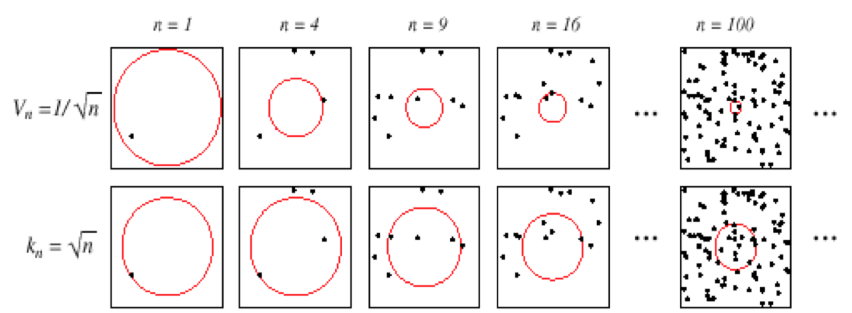
\includegraphics[scale=0.5]{img/px.png}
\caption{Metodi per la stima di densità di probabilità}
\label{px}
\end{figure}

\section{Parzen Windows}
L'approccio denominato \emph{Parzen Windows} può essere introdotto assumendo che la regione $\mathcal{R}_n$ è un ipercubo a $d$ dimensioni. Se $h_n$ è la lunghezza del lato dell'ipercubo allora il suo volume è dato da
\begin{equation}
V_n = h_n^d
\end{equation}
A questo punto viene introdotta la funzione finestra, la quale dice: se un campione rientra in un cubo assume valore 1 altrimenti assume valore 0.  
\[
\varphi(\mathbf{u})=
\begin{cases}
1 & \text{se} \ \abs{u_j} \leq 1/2\\
0 & \text{altrimenti}
\end{cases} 
\quad \quad \quad
j = 1, \dots, d.
\]
Facciamo un esempio a due dimensioni ed immaginiamo un quadrato centrato nell'origine, allora il valore delle due dimensioni deve essere $\abs{u_j} \leq 1/2$ per poter rientrare all'interno del quadrato, altrimenti si trova al di fuori. In questo caso è stato assunto che il lato abbia dimensione unitaria e che l'ipercubo sia centrato nell'origine. Volendo applicarla al caso generale è necessario traslare nell'origine e poi dividere per $h_n$, quindi la funzione finestra divente $\varphi((\mathbf{x} - \mathbf{x}_i)/h_n)$. Una volta ottenuta la funzione finestra per il caso generale la applico a tutti i punti per vedere quanti campioni rientrano all'interno della regione. Il che può essere calcolato con la sommatoria per tutti gli $i=1$
\begin{equation}
k_n = \sum_{i=1}^n \varphi \left ( \frac{\mathbf{x} - \mathbf{x}_i}{h_n} \right )
\end{equation}
così $k_n$ lo calcolo e non si fa nessuna ipotesi, mentre si fa l'ipotesi sul volume che come abbiamo detto è uguale a $h_n^d$. Sostituiamo $k_n$ nella formula originaria
\begin{equation}
p_n(\mathbf{x}) = \frac{k_n/n}{V_n}
\end{equation}
e ottengo
\begin{equation}\label{stima}
p_n(\mathbf{x}) = \frac{1}{n} \sum_{i=1}^n \frac{1}{V_n}\varphi \left ( \frac{\mathbf{x} - \mathbf{x}_i}{h_n} \right )
\end{equation}
La stima appena vista è basata sul concetto del conteggio del numero di campioni di training contenuti in un volume prefissato, quindi la stima della distribuzione di probabilità è espressa come somma di $N$ contributi, ciascuno dei quali è associato ad un singolo campione, ed il singolo contributo è espresso da una funzione $\varphi(\mathbf{u})$ che in generale non è rettangolare ($\varphi(\mathbf{u})$ ma assume valori continui. Si costruisce quindi la stima mediante l'equazione \ref{stima}. La funzione  $\varphi(\mathbf{u})$ è detta finestra di Parzen o \emph{kernel}.\\

\noindent Affinchè lo stimatore di Parzen abbia significato, è necessario imporre vincoli sul kernel $\varphi(\mathbf{u})$. Una condizione necessaria e sufficiente affinchè la stima di Parzen sia effettivamente una distribuzione di probabilità, è che la stessa funzione \emph{kernel} sia una distribuzione di probablità, ossia una funzione non-negativa
\begin{equation}
\varphi(\mathbf{x}) \geq 0
\end{equation}
e normalizzata
\begin{equation}
\int \varphi(\mathbf{u}) \ d\mathbf{u} = 1
\end{equation}
Definiata la funzione $\delta_n(\mathbf{x})$
\begin{equation}
\delta_n(\mathbf{x}) = \frac{1}{V_n} \varphi \left ( \frac{\mathbf{x}}{h_n} \right )
\end{equation}
allora la distribuzione di probabilità può essere scritta anche in un altra forma
\begin{equation}
p(\mathbf{x}) = \frac{1}{n} \sum_{i=1}^n \delta_n(\mathbf{x} - \mathbf{x}_i)
\end{equation}
Osserviamo come cambia la finestra di parzen al variare di $k_n$. I vari casi sono mostrati in figura \ref{parzen}.
\begin{figure}
\centering
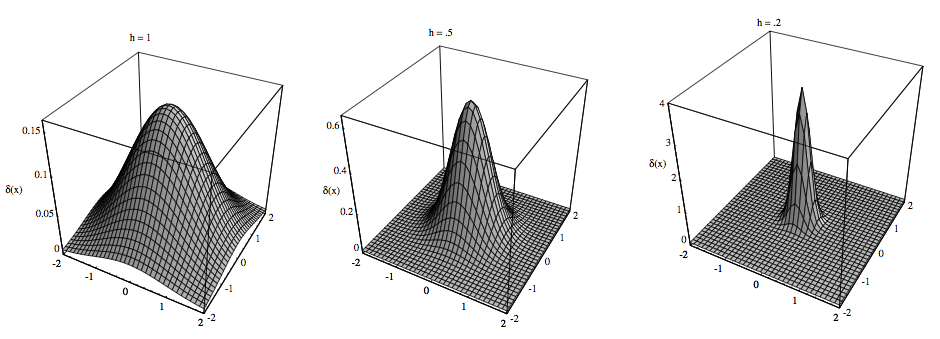
\includegraphics[scale=0.4]{img/parzen.png}
\caption{Finestre di parzen con $k_n$ variabile}
\label{parzen}
\end{figure}
Diminuendo $h_n$ il volume diventa più piccolo e di conseguenza $\delta_n$ ha un picco maggiore, di volta in volta che $h_n$ diminuisce il picco aumenta, quindi per $h_n$ tendente a zero diventa proprio la delta di dirac. Se invece $h_n$ è grande allora assume la forma di una gaussiana con varianza molto ampia ma con lo svantaggio che è poco rappresentativa dei pattern, quindi potrebbe essere che la distribuzione di probabiità non è costante di conseguenza stiamo perdendo molte informazioni dei pattern all'interno di questa regione (Regione grade equvale a perdita di informazioni). Analogamente invece $h_n$ è troppo piccolo allora guardiamo molti dettagli e nel tendere alla delta di dirac è come se stessimo osservando un singolo campione. Ritornando alla discussione sulla convergenza, bisogna tener conto della convergenza della sequenza delle variabili casuali, dato che per ogni fissato $\mathbf{x}$ il valore di $p(\mathbf{x})$ dipende dai campioni $\mathbf{x}_1, \dots, \mathbf{x}_n$. Quindi se la media di $p_n(\mathbf{x})$ è $\bar{p}_n(\mathbf{x})$ e la varianza è $\sigma^2_n(\mathbf{x})$. Allora la stima di $p_n(\mathbf{x})$ converce a $p(\mathbf{x})$ se
\begin{equation}
\lim_{n \to \infty} \bar{p}_n(\mathbf{x}) = p(\mathbf{x})
\end{equation}
e
\begin{equation}
\lim_{n \to \infty} \sigma^2_n(\mathbf{x}) = 0
\end{equation}

\subsection{Esempi}
\'E interessante vedere come  si comporta il metodo \emph{parzen windows} ed in particolare osservare l'effetto della funzione finestra. Consideriamo il caso in cui $p(\mathbf{x})$ è una distribuzione normale monovariata a media zero e varianza unitaria. L funzione finestra avrà la seguente forma
\begin{equation}
\varphi(u) = \frac{1}{\sqrt{2\pi}} e^{-u^2/2}
\end{equation}
dato $h_n = h_1/\sqrt{n}$. Allora $p_n(x)$ è una distribuzione di densità centrata sui campioni
\begin{equation}
p_n(x) = \frac{1}{n} \sum_{i=1}^n \frac{1}{h_n} \varphi \left ( \frac{x - x_i}{h_n} \right)
\end{equation}
\begin{figure}
\centering
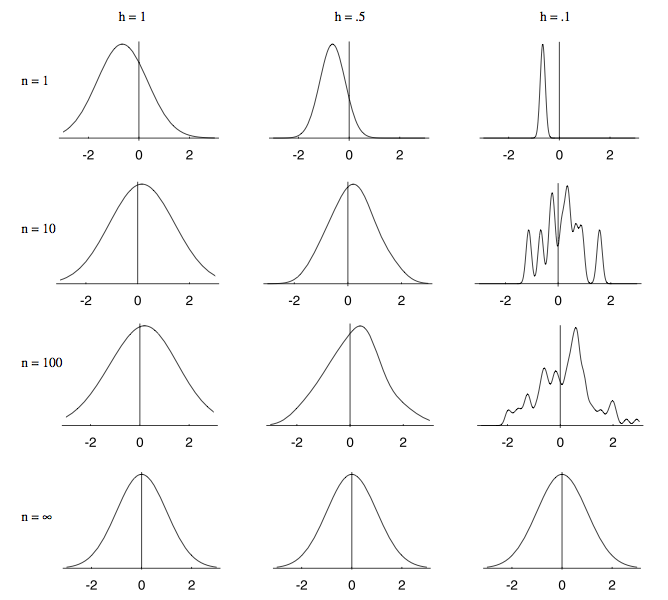
\includegraphics[scale=0.5]{img/parzen1.png}
\caption{Stima mediante la tecnica \emph{Parzen window} di una distribuzione normale monovariata facendo variare il parametro $h_1$ ed il numero di campioni $n$}
\label{parzen1}
\end{figure}
Effettuando un pò di calcoli sono stati ottenuti i risultati mostrati in figura \ref{parzen1}. I risultati dipendono sia da $h_1$ che da $n$. Per $n=1$ e $h_1=1$ è semplicemente una gaussiana centrata sul primo campione, quindi una visione sfocata \emph{out-of-focus} della distribuzione. Per $n=10$ e $h_1 = 0.1$ osserviamo che si può distinguere il contributo di ogni campione cosa che non avviene nel caso in cui $h_1=1$ e $h_1=0.5$. 

\subsection{Classificazione}
Una volta stimata la densità di probabilità allora la classificazione viene effettuata mediante una stima a massima probabilità a posteriori (MAP). Le regioni di decisioni dipendono dalla scelta che si fa per la funzione finestra. In generale, l'errore è basso scegliendo finestre con dimensione piccola.

\section{$k_n$-Nearest Neighbor estimation}
 Un rimedio al problema della dimensione della finestra di parzen è quello di considerare il volume in funzione dei campioni di training. Per esempio, per stimare la $p(\mathbf{x})$ di un insieme di campioni di training, possiamo centrare la regione in $\mathbf{x}$ e farla crescere finchè ingloba $k_n$ campioni, dove $k_n$ è specificato in funzione di $n$. Questi campioni sono i $k_n$ \emph{nearest-neighbor} di $\mathbf{x}$. Se vicino il campione $\mathbf{x}$ la densità è alta allora la cella sarà piccola, viceversa se la densità è bassa allora si avrà una regione grande. In entrambi i casi se prendiamo
 \begin{equation}\label{stima1}
p_n(\mathbf{x}) = \frac{k_n/n}{V_n}
\end{equation}
vogliamo che sia $k_n$ ed $n$ tendono ad infinito dato che ci assicura che $k_n/n$ sarà una buona stima di probabilità che un punto cadrà all'interno del volume $V_n$. Comunque, vogliamo anche che $k_n$ cresce lentamente finchè la dimensione della cella non include i $k_n$ campioni. \'E chiaro che dalla \ref{stima1} il rapporto $k_n/n$ tende a zero. Si può dimostrare che le condizioni $\lim_{n \to \infty} k_n = \infty$ e $\lim_{n \to \infty} k_n/n = 0$ sono necessarie e sufficienti affinchè $p_n(\mathbf{x})$ converge a $p(\mathbf{x})$. Se poniamo $k_n=\sqrt{n}$ e assumiamo che $p_n(\mathbf{x})$ è una buona approssimazione di $p(\mathbf{x})$ allora dall'eq. \ref{stima1} otteniamo che $V_n \simeq \/(\sqrt{n} \ p(\mathbf{x}))$. Così $V_n$ ha ancora la forma $V_1/\sqrt{n}$, ma il volume iniziale è determinato dalla natura dei dati piuttosto che da una scelta arbitraria. \'E interessante notare che nonostante $p_n(\mathbf{x})$ è continua la sua pendenza (o gradiente) non lo è. Inoltre i punti di dscontinuità corrispondono ai punti stessi (Fig. \ref{knn1} e \ref{knn2}).

\begin{figure}
\centering
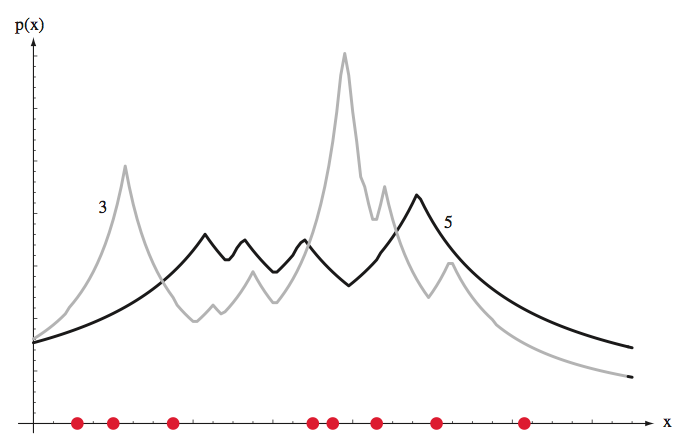
\includegraphics[scale=0.33]{img/knn1.png}
\caption{}
\label{knn1}
\end{figure}

\begin{figure}
\centering
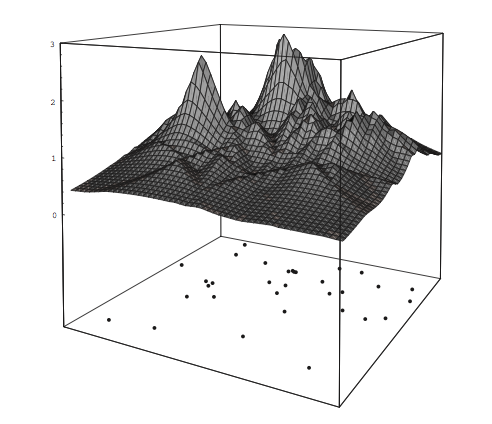
\includegraphics[scale=0.5]{img/knn2.png}
\caption{}
\label{knn2}
\end{figure}

\subsection{$K_n$-Nearest-Neighbor and Parzen Window Estimation }
Nel caso in cui $n=1$ allora $k_n = \sqrt{n} = 1$ e quindi i questo caso la stima diventa
\begin{equation}
p_n(x) = \frac{1}{2\abs{x-x_1}}
\end{equation}
\'E il caso in cui il numero di campioni più prossimi ad $x$ sia $1$, portando ad una tecnica denominata \emph{one-nearest-neighbor}

\subsection{Estimation of \emph{A Posteriori} Probabilities}
Le tecniche discusse nelle precedenti sezioni possono essere usate per stimare la probabilità a posteriori $P(\omega_i|\mathbf{x})$ da un insieme di $n$ campioni etichettati usando gli stessi campioni per stimare le densità coinvolte. Supponiamo di utilizzare una volume $V$ intorno ad $\mathbf{x}$ e catturare i $k$ campioni, $k_i$ di questi sono etichettati con $\omega_i$. La stima della probabilità congiunta $p(\mathbf{x} \cap \omega_i)$ è 
\begin{equation}
p_n(\mathbf{x} \cap \omega_i) = \frac{k_i/n}{V}
\end{equation}
quindi la stima di $P(\omega_i | \mathbf{x})$ è
\begin{equation}
P_n(\omega_i | \mathbf{x}) = \frac{p_n(\mathbf{x} \cap \omega_i)}{\sum_{j=1}^c p_n(\mathbf{x} \cap \omega_j)} = \frac{k_i}{k}
\end{equation}
La probabilià a posteriori che il campione appartenga alla classe $\omega_i$ è data dal rapporto tra il numero campioni etichettati con $\omega_i$ ed i campioni $k$ all'interno del volume. Per la scelta della grandezza della cella è chiaro che possiamo usare sia l'approccio basato sulle finestre di parzen che quello basato sul $k_n$\emph{-nearest-neighbor}. Nel primo caso $V_n$ deve essere specificato come funzione di $n$, come $V_n = 1/\sqrt{n}$. Nel secondo caso, $V_n$ viene esteso fino a racchiudere un determinato numero di campioni, es. $k = \sqrt{n}$. 

\subsection{The Nearest-neighbor rule}
Sia $\mathcal{D}^n = \{\mathbf{x}_1, \dots, \mathbf{x}_n \}$ un insieme di $n$ campioni dei quali conosciamo la classe di appartenenza (approccio supervisionato), preso $\mathbf{x}' \in \mathcal{D}^n$ come più vicino prossimo al campione $\mathbf{x}$ che è un campione di test (quindi non appartiene al dataset). La regola nearest-neighbor assegna ad $\mathbf{x}$ l'etichetta di $\mathbf{x}'$. Il tasso di errore è certamente maggiore di quello della regola di bayes, cioè quella del minimo possibile, però si dimostra che il tasso di errore è al più due volte l'errore di bayes, cioè è limitato superiormente da due volte l'errore di bayes. L'errore di bayes è molto piccolo, quindi moltiplicato per due è ancora piccolo. Questo è il vantaggio che può dare il nearest-neighbor con $k=1$, quindi costo computazionale bassissimo con grossa resa, dato che per $n$ tendende ad infinito la probabilità di $p(\omega_i|\mathbf{x}') \simeq p(\omega_i|\mathbf{x})$, cioè i vicini hanno probabilità a posteriori costanti. Inoltre se $p(\omega_m|\mathbf{x}') \simeq 1$, qundi molto alta, allora in tal caso il comportamento del classificatore nearest-neighbor è uguale al comportamento di bayes. 
\begin{figure}
\centering
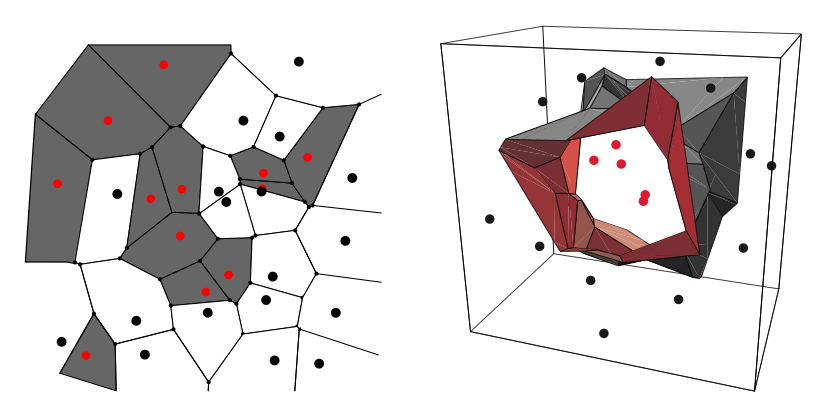
\includegraphics[scale=0.4]{img/voronoi.png}
\caption{Tassellazione di voronoi, le frontiere di decisione sono come superfici di diamanti}
\label{voronoi}
\end{figure}
Stiamo dicendo che una regola di classificazione banale ha un comportamento molto valido. Generalizzando, il \emph{k-nearest-neighbord} assegna ad $\mathbf{x}$ l'etichetta del campione più frequentemente rappresentato dei $k$ campioni più vicini. L'algoritmo conduce quindi ad un partizionamento, una cosa interessante in quanto ho delle celle intorno ad ogni campione $\mathbf{x}$. La suddivisione delle celle viene definita tassellazione di voronoi, fondamentalmente è un partizionamento senza sovrapposizione delle celle (Fig. \ref{voronoi}). \\

\noindent Nota: Se aumento il numero di $k$ vicini le regioni sono dense e i picchi si abbassano, invece se $k$ diminuisce allora ci sono più picchi.


%

%%%%%%%%%%%%%%%%%%%%% chapter.tex %%%%%%%%%%%%%%%%%%%%%%%%%%%%%%%%%
%
% sample chapter
%
% Use this file as a template for your own input.
%
%%%%%%%%%%%%%%%%%%%%%%%% Springer-Verlag %%%%%%%%%%%%%%%%%%%%%%%%%%

\chapter{Unsupervised Learning and clustering}
\section{Vantaggi dell' Unsupervised Learning}
%Fino ad ora abbiamo assunto che i campioni di training utilizzati per progettare un classificatore sono stati etichettati in base alla classe di appartenenza. Le procedure che utilizzano campioni etichettati sono detti \emph{supervised}. Adesso verranno analizzate un numero di procedure \emph{unseupervised}, le quali usano campioni non etichettati, quindi non abbiamo una conoscenza del loro stato della natura. Ci sono cinque ragioni di base per cui si potrebbe essere interessati ad una procedura \emph{unsupervised}. Primo, collezionare ed etichettare un grande numero di campioni potrebbe risultare molto costoso. Per esempio, registrare le voci è semplice, ma un etichettatura del parlato - quindi segnare quale parola o fonema è stato pronunciato per ogni istante - può essere molto costoso in termini di tempo. Se un classificatore potrebbe essere crudelmente progettato su un piccolo insieme di campioni etichettati e poi metterlo appunto permettendogli di essere eseguito senza supervisione su un grande insieme di campioni non etichettati, molto tempo e problemi possono essere evitati. Secondo, si potrebbe pensare di procedere al contrario: addestrare un grande numero di dati non etichettati e poi usare un metodo per etichettare i gruppi (\emph{cluster}) di dati trovati.Questo è il tipico funzionamento di un applicazione di \emph{data mining}, dove i contenuti di un grande database non sono conosciuti in anticipo. Terzo, in molte applicazioni le caratteristiche dei pattern possono cambiare molto lentamente nel tempo, per esempio in un classificatore di alimenti le cose potrebbero cambiare in base alle stagioni. Se questi cambiamenti possono essere rilevati dal classificatore eseguendolo in modo \emph{unsupervised}. Quarto, possiamo usare i metodi \emph{unsupervised} per trovare della \emph{feature} che saranno utili poi per la classificazione. Infine, nella fase iniziale di investigazione dei dati potrebbe essere utile per eseguire un analisi esplorative dei dati ottenendo la comprensione della natura o della struttura dei dati. La scoperta di sottoclassi distinte - \emph{cluster} i cui membri sono molto simili l'uno con l'altro - o grandi distanze tra le caratteristiche attese potrebbero suggerirci che altera in modo significativo l'approccio di progettare il classificatore. \\
%Dovremmo incominciare con delle assunzioni molto restrittive, quindi che la forma delle distribuzioni di probabilità sono conosciute e l'unica cosa che deve essere addestrata sono i valori sconosciuti del vettore dei parametri. \'E abbastanza interessante notare che la soluzione formale di questo problema si rivelerà essere abbastanza identica al problema affrontato per il caso \emph{supervised} nel cap. \ref{tecnicheParametriche}.\\

Fino ad ora abbiamo assunto che i campioni di training utilizzati per progettare un classificatore sono stati etichettati in base alla classe di appartenenza. Quindi si ha a disposizione un insieme di dati dei quali conosciamo la loro natura di appartenenza. Le procedure che operano su quest'insieme di dati sono dette \emph{unsupervised}. Questa modalità è utilizzata per una serie di ragioni. Esempio, raccogliere ed etichettare un gran numero di campioni può risultare molto costoso, in alcuni casi potrebbe essere non fattibile in quanto non si ha a disposizione un esperto. Inoltre da un punto di vista statistico è più facile affrontare il problema nel caso non supervisionato che nel caso supervisionato, nel senso che è molto difficile etichettare i campioni da parte di un esperto che molto spesso lo riesce a fare soltanto per un numero di campioni molto ridotto, problema invece che non si ha nel caso \emph{unsupervised} in quanto il numero di campioni non etichettato può anche crescere a dismisura dato che non è vincolato dal lavoro ulteriore di un esperto che etichetta i campioni. Quindi dal punto di vista statistico la rappresentatività dei dati non etichettati, tipicamente è maggiore dei dati etichettati, inoltre i metodi non supervisionati possono essere utilizzati anche per l'estrazione di caratteristiche. 
Un esempio è quando non si conosce la sorgente dei dati, tipicamente i dati vengono raccolti da sensori e non si ha neanche un esperto che riesce ad etichettare i dati (\emph{fetaure}), quindi l'approccio non supervisionato oltre ad apparire come un approccio per la classificazione di dati non etichettati  potrebbe apparire anche come un processo di preelabrazione dei dati. Per esempio quando si ha a disposizione una quantità enorme di dati, questi vengono analizzati con la condizione che non si sa da dove derivano e quale è l'etichetta. Quindi si ha a disposizione  molti campioni per effettuare un analisi statistica dei dati senza l'ausilio degli esperti, questo processo produce un insieme ridotto delle osservazioni e sono queste quelle che verranno poi sottoposte all'analisi. Sotto questo aspetto Il processo di classificazione non supervisionato non è un processo di classificazione ma un processo di estrazione di carattaristiche. Le tecniche che verranno utilizzate, sono tecniche di \emph{data mining} (investigare i dati). L'analisi dei dati per esplorazione (mining) può risultare utile alla comprensione della natura e struttura dei dati, quindi solo dopo aver effettuato un esplorazione attenta dei dati è possibile analizzarli e quindi sarà possibile poi dire si i dati analizzati corrispondono ad un determinato processo.\\

\section{Introduzione}
Stiamo nel caso in cui l'apprendimento è non supervisionato, quindi il caso in cui i campioni che abbiamo a disposizione non sono etichettati. \'E un caso abbastanza generale poiché è molto difficile raccogliere ed etichettare un gran numero di campioni, in quanto effettuare tali operazioni è costoso in termini di tempo, ma soprattutto è costoso in termini di energie di esperti del settore spese per poter operare un etichettatura dei campioni. Quindi in alcuni casi abbiamo una raccolta di dati, anche abbastanza considerevole, non etichettati però rappresentativi di fenomeni abbastanza complessi che devono essere studiati. Studiare un fenomeno non significa soltanto riuscire a determinare la struttura, ma molto spesso significa proprio rilevare eventi che non sono noti, rilevare anomalie che rappresentano eventi significativi, per cui scoprire caratteristiche dai dati è l'obiettivo dell'unsupervised learning. Il termine apprendimento è legato al fatto che i parametri delle distribuzioni di probabilità dei modelli non sono noti e bisogna renderli noti soltanto dopo una fase di addestramento di un sistema che si va a progettate. Per prima cosa si dovrebbe progettare un sistema di classificazione assumendo che si basi sul criterio MAP, quindi la probabilità a posteriori segue la regola di Bayes, però le probabilità che entrano in gioco nella regola di Bayes non sono note, non sono note le proprietà a priori ed in particolare le probabilità condizionate ovvero la verosomiglianza e di conseguenza se non sono note queste non è nota neanche l'evidenza, ovvero il denominatore della regola di Bayes, quindi di conseguenza non è nota la probabilità a posteriori. L'ipotesi in questo caso, come abbiamo già fatto per l'apprendimento supervisionato è quella di avere la conoscenza del modello, cioè di avere conoscenza della distribuzione di probabilità dei dati. \'E un ipotesi forte in quanto ci appelliamo al teorema del limite centrale il quale dice che su un numero di campioni infinito le distribuzioni di probabilità tendono ad essere gaussiane, ci limitiamo pertanto a stimare o meglio ad apprendere i parametri delle distribuzioni di probablità gaussiane, che  nella maggior parte dei casi sono gaussiane multivariate caratterizzate da una media e da una matrice di covarianza. Un punto essenziale è come scoprire le regolarità dei dati, cioè se i dati che io raccolgo si comportano in modo regolare, dal punto di vista matematico regolare significa che è possibile interpolare questi dati attraverso delle funzioni matematiche che appaiono funzioni regolari, quindi scoprire le regolarità vuol dire scoprire un modello di comportamento che è assolutamente importante per il rilevamento di anomalie. Praticamente a cosa serve la teoria non supervisionata ed il clustering? Immaginiamo di avere una raccolta di dati considerevole, etichettare questi dati è improponibile, avere conoscenza di cosa corrispondono questi dati è altrettanto improponibile allora l'esperto non lo si chiama proprio, non viene proprio interpellato per guardare i dati, si fa una scrematura, ovvero una pulizia dei dati, quindi si studiano le regolarità dei dati attraverso le tecniche di unsupervised learning o clustering in modo tale che i prototipi dei cluster che poi vengono identificati (il raggruppamento) verranno poi posti all'attenzione degli esperti, cioè quindi non i dati stessi ma i prototipi dei cluster i cui ho suddiviso i dati, naturalmente i prototipi dei cluster in cui ho suddiviso i dati sarà in numero nettamente minore dei dati da osservare e quindi porta ad una realizzazione del procedimento di etichettatura da parte di un esperto. Pertanto quello che stiamo dicendo è che molto spesso l'apprendimento non supervisionato è una fase di elaborazione, cioè quella fase di analisi dei dati che viene prima di una analisi più attenta dei dati stessi. Quindi ad un procedimento non supervisionato quasi sempre segue un procedimento supervisionato. In alcuni casi però è possibile anche che il risultato di un apprendimento non supervisionato sia già sufficiente per la comprensione del dataset e quindi l'esperto non viene interpellato. Quando i pattern appaiano molto densi allora il clusetring risulta essere molto agevole, quindi questa procedura è molto utile quando di dati sono densamente distribuiti intorno ad un prototipo o centroide. Quando invece i dati si distribuiscono in modo non così denso intorno ad un centroide allora è molto più difficile determinare i centroidi, è anche molto più difficile determinare i veri cluster e quindi è necessaria una fase di etichettatura. L'apprendimento non supervisionato rappresenta una grossolana suddivisione dei dati in gruppi. Il problema va però affrontato in un modo formalmente corretto.

\section{Mixture Densities and Identifiability}
Cominciamo con l'assunzione che conosciamo la completa struttura probabilistica del problema, con la sola eccezione di non conoscere i valori di alcuni parametri. Per essere più specifici, facciamo le seguenti assunzioni:

\begin{enumerate}
\item I campioni provengono un numero di $c$ classi che conosciamo
\item Le probabilità a priori $P(\omega_j)$ per ogni classe $j=1, \dots, c$ sono conosciute
\item Le densità di probabilità sono conosciute $p(\mathbf{x}|\omega_j , \mathbf{\Theta}_j)$
\item Valori dei vettori dei parametri $\mathbf{\Theta}_1, \dots, \mathbf{\Theta}_c$ sono sconosciuti
\item Le etichette per ogni categoria sono sconosciute
\end{enumerate}
A differenza dello studio effettuato nell'apprendimento supervisionato che veniva effettuato per classi, qui non conosciamo le classi di appartenenza, e quindi deve essere fatto su tutti i dati ipotizzando che i dati provengono da $c$ classi. Ma non sappiamo quali sono le classi perchè i pattern non sono etichettati. Si ipotizza che la distribuzione di probabiltà non è altro che una combinazione lineare delle distribuzioni di probabilità delle singole classi che però non sono note. Immagino che i dati provengono da $c$ classi, non si è a conoscenza di quali sono le classi, ma si sa  soltanto che la distribuzione di probabilità per ogni classe è per esempio una gaussiana multivariata, di cui non conosco ne la media ne la matrice di covarianza per ogni classe. Naturalmente poiché i dati non sono etichettati non posso fare un analisi per classe, ma devo fare un analisi di tutti i dati. Allora immagino che la distribuzione di probabilità totale dei dati non è altro che una combinazione lineare della distribuzione di probabilità per ogni singola classe, che prende il nome di mixtura di densità di probabilità, che nel caso di gaussiane prende il nome di mixture di gaussiame (MOG). L'evidenza $p(\mathbf{x})$, cioè la distribuzione di probabilità di un pattern qualsiasi $\mathbf{x}$ indipendentemente  da quale classe apparitene non è altro che la probabilità marginale delle probabilità congiunte. Posso certamente dire che 
\begin{equation}\label{93}
p(\mathbf{x}) = \sum_{j=1}^c p(\mathbf{x}, \omega_j)
\end{equation}
questa non è altro che la distribuzione di probabilità marginale della distribuzione di probabilità congiunta di $p(\mathbf{x}, \omega_j)$, ricordando che per la distribuzione di probabilità congiunta (la tabella a doppia entrata) la probabilità marginale si calcola per colonne o per righe. La \ref{93} è possibile riscriverla come
\begin{equation}
p(\mathbf{x}) = \sum_{j=1}^c p(\mathbf{x}|\omega_j) P(\omega_j)
\end{equation}

\noindent Assumiamo che i campioni sono stati ottenuti selezionando lo stato della natura $\omega_j$ con probabilità $P(\omega_j)$ e poi selezionando un osservazione $\mathbf{x}$ in accordo con la distribuzione di probabilità $p(\mathbf{x}|\omega_j, \mathbf{\Theta}_j)$. Così, la densità di probabilità per i campioni è data da
\begin{equation}
p(\mathbf{x}|\mathbf{\Theta}) = \sum_{j=1}^c p(\mathbf{x}|\omega_j, \mathbf{\Theta}_j) P(\omega_j)
\end{equation}
dove $\mathbf{\Theta} = (\mathbf{\Theta_1}, \dots, \mathbf{\Theta}_c)^t$, non è altro un vettore di vettori di parametri. Quindi ogni $\mathbf{\Theta}_j$ è un vettore di parametri, per fare un esempio nel caso di una gaussiana $\mathbf{\Theta}_j$ non è altro che il vettore costituito da media e matrice di covarianza della $j$-esima distribuzione gaussiana multivariata. Per ovvie ragioni, la funzione di densità in questa forma è chiamata \emph{mixture density}, le distribuzioni di probabilità condizionate sono chiamate \emph{component density} e le probabilità a priori sono chiamate \emph{mixing parameters}. L'obiettivo base sarà quello di usare i campioni che seguono la \emph{mixture density} per stimare il vettore parametri sconosciuti $\mathbf{\Theta}$.  Se l' obiettivo è la classificazione allora una volta trovato $\mathbf{\Theta}$ possiamo decomporre la mixtura in tante componenti e usare un classificatore MAP (\emph{maximum a posteriori}) sulle densità derivate. Prima di cercare una soluzione a questo problema, ci chiediamo comunque se è possibile o meno ricavare $\mathbf{\Theta}$ dalle mixture. Supponiamo che abbiamo un illimitato numero di campioni e che usiamo un metodo non parametrico della sezione \ref{metodinonparametrici} per determinare il valore di $p(\mathbf{x}|\mathbf{\Theta})$ per ogni $\mathbf{x}$. Se c'è un solo valore di $\mathbf{\Theta}$ che sarà prodotto dai valori osservati per $p(\mathbf{x}|\mathbf{\Theta})$, allora la soluzione è possibile in linea si principio, invece se molti valori di $\mathbf{\Theta}$ possono produrre gli stessi valori per $p(\mathbf{x}|\mathbf{\Theta})$, allora non ci sono speranze di ottenere una soluzione unica.\\
Queste considerazioni   ci portano alla seguente definizione: Una funzione di densità $p(\mathbf{x}|\mathbf{\Theta})$ è detta \emph{identificabile} se $\mathbf{\Theta} \neq \mathbf{\Theta}'$ implica che esiste un $\mathbf{x}$ tale che $p(\mathbf{x}|\mathbf{\Theta}) \neq p(\mathbf{x}|\mathbf{\Theta}')$, questo significa che quando si stimano i $\mathbf{\Theta}$ si potrebbe ottenere per differenti valori di $\mathbf{\Theta}$ la stessa distribuzione di probabilità, cosa che non deve accadere altrimenti il procedimento non va a buon termine.
Facciamo un semlice esempio dove si considera il caso in cui $x$ è binario (quindi può assumere $0$ o $1$) e $P(x|\mathbf{\Theta})$ è una mixtura di due binomiali
\begin{equation}
\begin{split}
P(x|\mathbf{\Theta}) &= \frac{1}{2} \Theta_1^x(1-\Theta_1)^{1-x} + \frac{1}{2}\Theta_2^x(1-\Theta_2)^{1-x}\\
&= \begin{cases}
\frac{1}{2}(\Theta_1 + \Theta_2) & \text{se} \ x =1\\
1 - \frac{1}{2}(\Theta_1 + \Theta_2) & \text{se} \ x = 0 
\end{cases} 
\end{split}
\end{equation}
\'E identificabile questa mixtura di densità? Presi due valori $\mathbf{\Theta}$ e $\mathbf{\Theta}'$ che sono diversi, esiste almeno un $x$ per cui $P(x|\mathbf{\Theta}) \neq P(x|\mathbf{\Theta}')$? \\
Supponiamo, per esempio, che conosciamo il valore di $P(x=1|\mathbf{\Theta}) = 0.6$ e quindi che $P(x=0|\mathbf{\Theta}) = 0.4$. Conosciamo la funzione $P(x|\mathbf{\Theta})$, ma non possiamo determinare $\mathbf{\Theta}$ e quindi non possiamo estrarre le componenti della distribuzione. Inoltre possiamo dire che $\Theta_1 + \Theta_2 = 1.2$. Come potremmo mai trovare dei valori $\Theta_1$ e $\Theta_2$ che identificano in modo inequivocabile la densità di probabilità se praticamente la loro somma in entrambi i casi è sempre uguae ad $1.2$? \\
Quindi è impossibile trovare una combinazione di parametri che sia identificabile.
Così, abbiamo un caso per il quale la distribuzione di mixture è completamente non identificabile, un caso per il quale la tecnica \emph{unseupervised} non può essere applicata in linea di principio. Questo tipo di problema si presenta comunemente nel caso di dati discreti, la presenza di molte componenti potrebbe rendere il problema abbastanza difficile, invece nel caso continuo, il problema è meno severo. \'E possibile mostrare che la mixtura di distribuzioni normali (mixtura di gaussiane) sono generalmente identificabili e i parametri di una semplice mixtura sono
\begin{equation}
p(x|\mathbf{\Theta}) = \frac{P(\omega_1)}{\sqrt{2\pi}} \exp \left[ -\frac{1}{2}(x-\Theta_1)^2 \right] + \frac{P(\omega_2)}{\sqrt{2\pi}} \exp \left[ -\frac{1}{2}(x-\Theta_2)^2 \right] 
\end{equation}
questa mixtura non può essere unicamente identificata se $P(\omega_1) = P(\omega_2)$, dato che $\Theta_1$ e $\Theta_2$ possono essere intercambiate senza cambiare $p(x|\mathbf{\Theta})$.

\section{Maximum Likelihood estimates}
Dato un insieme $\mathcal{D}= \{\mathbf{x}, \dots, \mathbf{x}_n \}$ composto da $n$ campioni, immaginiamo $n$ che sia infinito o comunque molto alto, i vettori sono \emph{i.i.d.}, dobbiamo inoltre ricordare che i campioni non sono etichettati e la mixtura di densità è
\begin{equation}
p(\mathbf{x}|\mathbf{\Theta}) = \sum_{j=1}^c p(\mathbf{x}|\omega_j, \mathbf{\Theta}_j) P(\omega_j)
\end{equation}
dove tutti i parametri del vettore $\mathbf{\theta}$ sono fissati ma non conosciuti. Conosciamo la provenienza dei dati ma non conosciamo ogni campione da quale classe proviene. Inoltre facciamo un altra ipotesi, che ogni classe ha un modello di distribuzione di probabilità noto, quindi possiamo immaginare che siano tutte gaussiane delle quali però non conosciamo le medie e le matrici di covarianza. L'obiettivo è quello di stimare i parametri di queste distribuzioni di probabiità, quindi di classi che non conosciamo la suddivisione. Allora non lavoriamo sul termine a destra perchè anche se diciamo che sono gaussiane non possiamo lavorare su media e covarianza di gruppi di dati che non conosco l'etichettatura, quindi si deve necessariamente lavorare sul termine a sinistra $P(\mathbf{x}|\mathbf{\Theta})$ augurandosi di poter fare qualche cosa anche sul termine a destra. Quindi $\mathbf{\Theta}$ è fisso ma non è noto, fisso significa che non cambia, è indipendentemente dal numero dei dati, una cosa poco relistica.\\
La verosomiglianza (\emph{likelihood}) dei campioni osservati è, per definizione, la probabilità congiunta
\begin{equation}
p(\mathcal{D}|\mathbf{\Theta})  =\prod_{k=1}^n p(\mathbf{x}_k|\mathbf{\Theta})
\end{equation}
$P(\mathcal{D}|\mathbf{\Theta})$ è la probabilità di tutto il training set dato $\mathbf{\Theta}$, ma abbiamo detto che  $\mathcal{D}= \{\mathbf{x}, \dots, \mathbf{x}_n \}$ ed essendo \emph{i.i.d.} posso scrivere $P(\mathcal{D}|\mathbf{\Theta})$ come produttoria. Dobbiamo trovare $\mathbf{\Theta}$, che in questo caso è il vettore dei parametri di tutti i parametri di tutte le classi, quindi tutte le medie e le covarianze di tutte le classi $c$ che ho a disposizione. Stiamo lavorando sul tutto il training set e non soltanto su una classe. L'obiettivo è massimizzare $p(\mathcal{D}|\mathbf{\Theta})$, quindi bisogna trovare il valore di $\mathbf{\hat{\Theta}}$ che sostituito nella distribuzione d probabilità $P(\mathcal{D}|\mathbf{\Theta})$ rendono più verosimile  
la distribuzione di probabilità a quella che è la reale distribuzione di probabilità, quindi una stima a massima verosomiglianza. La stima a massima verosomiglianza  di $\mathbf{\hat{\Theta}}$ è proprio il valore di $\mathbf{\Theta}$ che massimizza $p(\mathcal{D}|\mathbf{\Theta})$.\\
Per massimizzare una funzione facciamo la derivata e si pone uguale a zero. In particolare se i parametri $\mathbf{\Theta}$ sono tanti, in questo caso sono $c$ vettori di parametrim, allora bisogna fare $kc$ derivate parziali dove $k$ è il numero di parametri per la distribuzione e nel caso gausiano $k=2$. 
Se assumiamo che $p(\mathcal{D}|\mathbf{\Theta})$ è una funzione differenziabile di $\mathbf{\Theta}$, allora è possibile dedurre alcune necessarie ed interessanti condizioni per $\mathbf{\hat{\Theta}}$. Dato $l$ il logaritmo della verosomiglianza, e dato $\mathbf{\nabla}_{\mathbf{\theta}_1}l$ il gradiente di $l$ rispetto a $\mathbf{\Theta}_i$, allora
\begin{equation}
l= \sum_{k=1}^n \ln p(\mathbf{x}_k|\mathbf{\Theta})
\end{equation}
e
\begin{equation}
\mathbf{\nabla_{\Theta_i}} l = \sum_{k=1}^n \frac{1}{p(\mathbf{x}_k|\mathbf{\Theta})} \mathbf{\nabla_{\Theta_i}} \left[ \sum_{j=1}^c p(\mathbf{x}_k| \omega_j, \mathbf{\Theta}_j) P(\omega_j) \right]
\end{equation}
Inoltre assumiamo che gil elementi di $\mathbf{\Theta}_i$ e $\mathbf{\Theta}_j$ sono indipendenti soltanto se $i \neq j$, e introducendo la probabilità a posteriori che è uguale a
\begin{equation}
P(\omega_i|\mathbf{x}_k, \mathbf{\Theta}) = \frac{p(\mathbf{x}_k|\omega_i, \mathbf{\Theta}_i)P(\omega_i)}{p(\mathbf{x}_k|\mathbf{\Theta})}
\end{equation}
osserviamo che il gradiente della $log-likelihood$ può essere riscritto in una forma interessante
\begin{equation}
\mathbf{\nabla_{\Theta_i}} l = \sum_{k=1}^n P(\omega_i|\mathbf{x}_k, \mathbf{\Theta}) \mathbf{\nabla_{\mathbf{\Theta}_i}} \ln p(\mathbf{x}_k|\omega_i, \mathbf{\Theta}_i)
\end{equation}
Poichè il gradiente deve svanire al valore di $\mathbf{\Theta}_i$ che massimizza $l$, la stima a massima verosomiglianza $\mathbf{\hat{\Theta}}_i$ deve soddisfare le condizioni
\begin{equation}\label{8}
\sum_{k=1}^n P(\omega_i|\mathbf{x}_k, \mathbf{\hat{\Theta}}) \mathbf{\nabla_{\Theta}}_i \ln p(\mathbf{x}_k|\omega_i, \mathbf{\hat{\Theta}}_i) = 0 \quad \quad \quad i=1, \dots, c
\end{equation}
Risolvendo quest'equazione per $\mathbf{\hat{\Theta}}_i$ troveremo la soluzione della massima verosomiglianza.\\
Non è difficile generalizzare questi risultati includendo le probabilità a priori $P(\omega_i)$ tra le quantità sconosciute. In questo caso del valore che massimizza $p(\mathcal{D|\mathbf{\Theta}})$
si estende su $\mathbf{\Theta}$ e $p(\omega_i)$, soggetti ad i seguenti vincoli
\begin{equation}
P(\omega_i) \geq 0 \quad \quad \quad i=1, \dots, c
\end{equation}
e
\begin{equation}
\sum_{i=1}^c P(\omega_i)  = 1 
\end{equation}
Denotiamo con $\hat{P}(\omega_i)$ la stima a massima verosomiglianza per $P(\omega_i)$, e denotiamo dato $\mathbf{\hat{\Theta}}_i$ la stima a massima verosomigliaza per $\mathbf{\Theta}_i$. \'E possibile dimostrare che se la funzione di verosomiglianza è differenziabile e se $\hat{p(\omega_i)\neq 0}$ per qualsiasi $i$, allora $\hat{P}(\omega_i)$ e $\mathbf{\hat{\Theta}}$ deve soddisfare
\begin{equation}\label{11}
\hat{P}(\omega_i) = \frac{1}{n} \sum_{k=1}^n \hat{P}(\omega_i | \mathbf{x}_k, \mathbf{\hat{\Theta}})
\end{equation}
e
\begin{equation}\label{12}
\sum_{k=1}^n \hat{P}(\omega_i|\mathbf{x}_k, \mathbf{\hat{\Theta}}) \mathbf{\nabla_{\mathbf{\Theta}_i}} \ln p(\mathbf{x}_k|\omega_i, \mathbf{\hat{\Theta}}_i) = 0
\end{equation}
dove
\begin{equation}\label{13}
\hat{P}(\omega_i|\mathbf{x}_k, \mathbf{\hat{\Theta}}) = \frac{p(\mathbf{x}_k|\omega_i, \mathbf{\hat{\Theta}}_i)\hat{P}(\omega_i)}{\sum_{j=1}^c p(\mathbf{x}_k|\omega_j, \mathbf{\hat{\Theta}}_j)\hat{P}(\omega_j)}
\end{equation}
Queste equazioni hanno la seguente interpretazione. L'equazione \ref{11} ci dice che la stima a massima verosomiglianza della probabilità di una categoria è la media su tutto l'intero dataset delle stime derivate da ogni campione - ogni campione è ugualmente pesato. L'equazione \ref{13} è correlata al teorema di Bayes, ma da notare che il numeratore dipende da $\mathbf{\hat{\Theta}}_i$ e non su tutti i $\mathbf{\hat{\Theta}}$.

\section{Application To Normal Mixtures}
\'E istruttivo vedere come questi risultati si applicano al caso in cui le distribuzioni sono gaussiane multivariate, $P(\mathbf{x}|\omega_i, \mathbf{\Theta}_i)\sim N(\mathbf{\mu}_i, \mathbf{\Sigma}_i)$. La tabella seguente illustra i casi che potrebbero verificarsi indicando con $(\times)$ i parametri conosciuti e con $(?)$ i parametri non conosciuti:

\begin{table}[ht]
\centering
\begin{tabular}{l cccccccccc}
\hline
Case & $\mathbf{\mu}_i$  & $\mathbf{\Sigma}_i$ & $\mathbf{P(\omega_i)}$ & $c$\\
\hline
 1 &  $?$  & $\times$  &    $\times$   &  $\times$  \\
 2 & $?$ & $?$ & $?$ &    $\times$   \\
 3 & $?$ & $?$ & $?$ & $?$ \\
\hline
\end{tabular}
\end{table}
\noindent Il caso 1 è il più semplice ed è quello che verra considerato in dettaglio. Il caso 2 è quello più realistico, mentre il terzo caso rappresenta il problema di quando ci troviamo di fronte quando tutti i dati sono completamente sconosciuti,purtroppo non è possibile risolvere il problema con la tecnica a massima verosomiglianza. 

\subsection{Case 1: Vettore media non conosciuto}
\'E noto tutto tranne la media, quindi l'unico parametro da stimare è $\mathbf{\mu}_i$, e naturalmente $\mathbf{\mu}_i = \mathbf{\Theta}_i$. Allora la verosomiglianza diventa $p(\mathbf{x}|\omega_i, \mathbf{\mu}_i)$ e la log-verosomiglianza, ovvero il logaritmo è
\begin{equation}
\ln p(\mathbf{x}|\omega_i, \mathbf{\mu}_i) = - \ln \left[ (2\pi)^{d/2} \abs{\mathbf{\Sigma}}^{1/2} \right] - \frac{1}{2}(\mathbf{x}-\mathbf{\mu}_i)' \mathbf{\Sigma}_i^{-1}(\mathbf{x}- \mathbf{\mu}_i) 
\end{equation}
adesso bisogna fare la derivata parziale rispetto a $\mathbf{\mu}_i$ allora il primo termine va a zero dato che è costante rispetto a $\mathbf{\mu}_i$, 
il secondo termine invece applicando semplici passaggi matematici otteniamo
\begin{equation}
- \frac{1}{2} \frac{(\mathbf{x}-\mathbf{\mu}_i)'(\mathbf{x}-\mathbf{\mu}_i)}{\mathbf{\Sigma}_i} = -\frac{1}{2} \frac{(\mathbf{x}-\mathbf{\mu}_i)^2}{\mathbf{\Sigma}_i}
\end{equation}
e quindi risolvendo questa semplice derivata e moltiplicando per $-1$ che è la derivata di $-\mathbf{\mu}_i$ otteniamo
\begin{equation}
\nabla_{\mu_i} \ln p(\mathbf{x}|\omega_i, \mathbf{\mu}_i) = \mathbf{\Sigma}_i^{-1}(\mathbf{x}-\mathbf{\mu}_i)
\end{equation}
una volta ottenuta la derivata allora va sostituita nella \ref{8} e va posta uguale a 0
\begin{equation}
\sum_{k=1}^n P(\omega_i|\mathbf{x}_k, \hat{\mathbf{\mu}}) \mathbf{\Sigma}^{-1}(\mathbf{x}_k - \mathbf{\hat{\mathbf{\mu}}}_i) = 0 \quad \quad \quad \text{dove} \ \ \hat{\mathbf{\mu}} = (\hat{\mathbf{\mu}}_1, \dots, \hat{\mathbf{\mu}}_c)^t
\end{equation}
da questa $\mathbf{\Sigma}_i$ è nota e quindi di conseguenza anche l'inversa $\mathbf{\Sigma}_i^{-1}$ è nota, $\mathbf{x}_k$ è noto e $\hat{\mathbf{\mu}}_i$ non è noto. Per un istante immaginiamo che $P(\omega_i|\mathbf{x}_k, \hat{\mathbf{\mu}})$ è noto, o meglio è quella probabilità aposteriori che riusciamo in modo iterativo a stimare di volta in volta, quindi ad un certo istante abbiamo una stima delle probabilità aposteriori, non abbiamo quella reale ma certamente una stima ce l'abbiamo, quindi è tra virgolette nota. Allora risolvendo rispetto a $\hat{\mathbf{\mu}}_i$ otteniamo
\begin{gather}
\sum_{k=1}^n P(\omega_i|\mathbf{x}_k, \hat{\mathbf{\mu}}) \mathbf{\Sigma}_i^{-1}(\mathbf{x}_k - \mathbf{\hat{\mathbf{\mu}}}_i) = 0\\
\sum_{k=1}^n P(\omega_i|\mathbf{x}_k, \hat{\mathbf{\mu}}) \mathbf{\Sigma}_i^{-1} \mathbf{x}_k - P(\omega_i|\mathbf{x}_k, \hat{\mathbf{\mu}}) \mathbf{\Sigma}_i^{-1} \mathbf{\hat{\mathbf{\mu}}}_i = 0\\
\sum_{k=1}^n P(\omega_i|\mathbf{x}_k, \hat{\mathbf{\mu}}) \mathbf{\Sigma}_i^{-1} \mathbf{x}_k = \sum_{k=1}^n P(\omega_i|\mathbf{x}_k, \hat{\mathbf{\mu}}) \mathbf{\Sigma}_i^{-1} \mathbf{\hat{\mathbf{\mu}}}_i \\
\mathbf{\hat{\mathbf{\mu}}}_i = \frac{\sum_{k=1}^n P(\omega_i|\mathbf{x}_k, \hat{\mathbf{\mu}}) \mathbf{\Sigma}_i^{-1} \mathbf{x}_k}{ \sum_{k=1}^n P(\omega_i|\mathbf{x}_k, \hat{\mathbf{\mu}}) \mathbf{\Sigma}_i^{-1}}
\end{gather}
$ \mathbf{\Sigma}_i^{-1}$ è nota e allora 
\begin{equation}
\mathbf{\hat{\mathbf{\mu}}}_i = \frac{\sum_{k=1}^n P(\omega_i|\mathbf{x}_k, \hat{\mathbf{\mu}})  \mathbf{x}_k}{ \sum_{k=1}^n P(\omega_i|\mathbf{x}_k, \hat{\mathbf{\mu}})}
\end{equation}
e possiamo osservare che $\mathbf{\hat{\mathbf{\mu}}}_i$ non è altro che la media ponderata degli $\mathbf{x}_k$ all'interno di una classe. Per cui,  come si può immaginare il valore di $P(\omega_i|\mathbf{x}_k, \hat{\mathbf{\mu}})$? Se sapessimo già da prima quali erano le appartenenze dei pattern ai gruppi allora era facile, bastava vedere quanti campioni stavano in ogni classe e il valore di quei campioni, quindi la porzione dei campioni che sta in una classe è $P(\omega_i|\mathbf{x}_k, \hat{\mathbf{\mu}})$. Adesso è lo stesso ragionamento, solo che poichè non conosciamo a priori quali sono le classi, ma sappiamo quante sono le classi, di volta in volta che facciamo la stima calcoliamo quanti campioni rientrano in questo gruppo, cioè fondamentalmente sommiamo i $P(\omega_i|\mathbf{x}_k, \hat{\mathbf{\mu}})$, ovvero le probabilità aposteriori che rappresentano la frazione dei campioni avente valore $\mathbf{x}_k$ e che appartengono alla $i$-esima classe sono i pesi di questa combinazione lineare e quindi della media ponderata.\\

\noindent Questo è un risultato analogo a quello che abbiamo ottenuto anche per l'apprendimento a massima verosomiglianza nel caso del supervisionato, poichè il primo caso che stiamo vedendo adesso è esattamente il primo caso nella massima verosomilianza del supervisionato, in quella situazione la media che si va a massimizzare era la media dei campioni appartenenti alla classe, quindi tutta questa base teorica per dire che il valor medio, ovvero la media della gaussiana che mi distribuisce o che modella la distribuzione dei dati di una classe la vado a calcolare semplicemente facendo la media campionaria (media dei pattern appartenenti alla classe). IN questo caso non conocsciamo quanti pattern sono in ogni classe ma è possibile stimarlo di volta in volta, e questa stima è la $P(\omega_i|\mathbf{x}_k, \hat{\mathbf{\mu}})$ che è possibile calcolare mediante la regola di Bayes 
\begin{equation}
P(\omega_i|\mathbf{x}_k, \hat{\mathbf{\mu}}) = \frac{ p(\mathbf{x}_k|\omega_i, \hat{\mathbf{\mu}}_i) P(\omega_i) }{ \sum_{j=1}^c p(\mathbf{x}|\omega_j, \hat{\mathbf{\mu}}_j) P(\omega_j)}
\end{equation}
fondamentalmente il processo è sempre iterativo, quindi abbiamo risolto il sistema di equazioni lineari, dove ne abbiamo $c$, nel caso particolare il cui il parametro da calcolare è $\mathbf{\mu}_i$. Quindi la soluzione è la media ponderata, il processo iterativo di queste stima lo facciamo lo stesso soltanto che poi ci accorgiamo che questo vettore medio ponderato cambia in virtù di quanti pattern metto nella classe (un procedimento simile al clustering k-means, parto da un centroide e di volta in volta il centroide si avvicina a quello che dovrebbe essere reale centroide del cluster ricalcolando il centroide di un cluster in modo iterativo), infatti le medie vengono calcolate in modo iterativo come 
\begin{equation}
\mathbf{\hat{\mathbf{\mu}}}_i(j+1) = \frac{\sum_{k=1}^n P(\omega_i|\mathbf{x}_k, \hat{\mathbf{\mu}}(j))  \mathbf{x}_k}{ \sum_{k=1}^n P(\omega_i|\mathbf{x}_k, \hat{\mathbf{\mu}}(j))}
\end{equation}
quindi la media al passo $j+1$ viene calcolata in virtù della media calcolata al passo $j$. Per gli informatici è un algoritmo \emph{greedy} mentre per i matematici è noto come tecnica del gradiente ascendente, ascendente perchè stiamo massimizzando la log-verosomiglianza dei dati.

\subsection{Case 2: Tutti i parametri non conosciuti}

In questo caso è noto soltanto il numero delle classi, quindi non conosciamo $P(\omega_i)$ e non conosciamo entrambi i parametri $\mathbf{\mu}_i$ e $\mathbf{\Sigma}_i$ delle gaussiane che modellano la distribuzione dei dati. Allora supponiamo che la verosomiglianza non è altro che una mixtura a due componenti
\begin{equation}
p(x|\mu, \sigma^2) =\frac{1}{2 \sqrt{2\pi} \sigma} \exp \left[ -\frac{1}{2} \left( \frac{x -\mu}{\sigma} \right)^2  \right]  + \frac{1}{2 \sqrt{2\pi}} \exp \left[ -\frac{1}{2}x^2 \right]
\end{equation}
quindi la funzione di verosomiglianza è rappresentata da questa mixtura e si nota che nella seconda si ha media pari a zero e varianza uguale ad uno (normale standardizzata). La verosomiglianza per $n$ campioni non è latro che il prodotto di $n$ densità $p(x_k|\mu, \sigma^2)$, quindi la $p(\mathcal{D}|\mu, \sigma^2)$ non è altro che la produttoria $p(\mathcal{D}|\mu, \sigma^2) = \prod_{k=1}^n p(x_k|\mu, \sigma^2)$. Supponiamo che $\mu$ iniziale sia pari ad un pattern $x_1$, quindi $\mu=x_1$, sostituendo vien fuori
\begin{equation}
p(x|\mu, \sigma^2) =\frac{1}{2 \sqrt{2\pi} \sigma} + \frac{1}{2 \sqrt{2\pi}} \exp \left[ -\frac{1}{2}x_1^2 \right]
\end{equation}
invece per il resto dei campioni invece non può che essere
\begin{equation}
p(x|\mu, \sigma^2) \geq \frac{1}{2 \sqrt{2\pi}} +  \exp \left[ -\frac{1}{2}x_k^2 \right]
\end{equation}
quindi
\begin{equation}
p(x_1, \dots, x_n | \mu, \sigma^2) \geq \left\{ \frac{1}{\sigma} + \exp \left[ -\frac{1}{2}x_1^2    \right] \right\} \frac{1}{(2\sqrt{2\pi})^n} \exp \left[ -\frac{1}{2} \sum_{k=2}^n x_k^2 \right]
\end{equation}
il tutto dipende da $\sigma$, se $\sigma$ tende a zero allora questa quantità tende ad infinito, la densità di probabilità di tutti i dati è maggiore o uguale della quantità che si trova a destra, se $1/\sigma$ tende all'infinito allora a maggior ragione il termine a sinistra tenderà all'infinito, o meglio si può dire che la verosomiglianza diventa arbitrariamente grande e quindi la soluzione a massima verosomiglianza sarebbe impossibile. Quindi la scelta della prima stima dei centroidi non deve essere casuale, deve essere mirata, altrimenti si può incorrere in problemi di questo tipo, cioè non è possibile che il procedimento di cui stiamo parlando vada a convergere. Ci sono delle soluzioni abbastanza importanti quando il numero dei massimi locali è finito, cioè quando la distribuzione di probabilità, quindi della verosomiglianza, non ha un solo massimo globale, ma questo massimo globale è il massimo dei massimi locali, e questo numero di massimi locali è un numero finito, allora in tal caso il problema si può risolvere, in quando vado a convergere per trovare il massimo locale. Riprendendo le equazioni \ref{11}-\ref{13}, si può individuare subito che la covarianza si può calcolare come una media ponderata ottenendo la stima per $\mathbf{\mu}_i, \mathbf{\Sigma}$ e $P(\omega_i)$    


\subsection{\emph{k}-Means Clustering}
Il \emph{k}-Means è un algoritmo utilizzato per classificare o dividere in $k$ gruppi i pattern descritti da un vettore delle caratteristiche. Il raggruppamento è svolto minimizzando la somma delle radici quadrate delle distanza fra i dati. I passi dell'algoritmo sono abbastanza semplici. Si inizia col determinare il numero di cluster $k$ che viene scelto in base agli scopi dell'applicazione. Per esempio se si tratta di un applicazione di riconoscimento di caratteri inglesi allora è opportuno scegliere $k=26$. Oltre al numero di cluster si scelgono anche $k$ centroidi che possono essere sia scelti casualmente dai dati già a disposizione oppure anche in modo casuale senza essere necessariamente un pattern dei dati. L'algoritmo è caratterizzato da tre passi e viene eseguito finchè non converge.

\begin{enumerate}
\item Si determinano i $k$ centrodi
\item Si calcola la distanza di ogni oggetto dal centroide
\item Si assegna un oggetto ad un gruppo in base alla distanza minima
\item Si ricalcolano i centroidi (calcolando una semplice media ) in base a i nuovi gruppi e si itera finchè i centroidi non rimangono invariati
\end{enumerate}
   
\subsection{Fuzzy \emph{k}-Means Clustering}
In ogni iterazione dell'algoritmo \emph{k}-Means classico si assume che ogni pattern viene assegnato ad un unico cluster. \'E possibile rilassare questa condizione assumendo che ogni campione $\mathbf{x}_j$ ha un grado di appartenenza, quindi secondo i concetti della logica \emph{fuzzy}. L'algoritmo Fuzzy \emph{k}-Means cerca il minimo globale della funzione costo
\begin{equation}
J_{fuz} = \sum_{i=1}^c \sum_{j=1}^n [ \hat{P} (\omega_i | \mathbf{x}_j,  \mathbf{\hat{\Theta}}) ]^b \norma{\mathbf{x}_j - \mathbf{\mu}_i}^2
\end{equation}
dove  $b$ è un parametro scelto libero per aggiustare il \emph{``blending''} (mescolanza) tra i clusters differenti. Se $b$ viene posto a 0 allora $J_{fuz}$ è semplicemente il criterio d'errore basato sulla somma delle radici quadrate con ogni pattern assegnato soltanto ad un cluster. Le probabilità di appartenenza ad un claster per ogni punto sono normalizzate nel seguente modo
\begin{equation}\label{30}
\sum_{i=1}^c \hat{P}(\omega_i | \mathbf{x}_j) = 1, \quad \quad \quad j=1, \dots, n
\end{equation}
Denotiamo con $\hat{P}_j$ la probabilità a priori di $\hat{P}(\omega_j)$, allora per trovare il minimo di $J_{fuz}$ abbiamo
\begin{equation}\label{31}
\partial J_{fuz} / \partial \mathbf{\mu}_i = 0 \quad \quad \quad \text{e} \quad \quad \quad \partial J_{fuz} / \partial \hat{P}_j = 0
\end{equation}
questo porta alla seguente soluzione
\begin{equation}\label{32}
\mathbf{\mu}_j = \frac{\sum_{j=1}^n [ \hat{P}(\omega_i | \mathbf{x}_j)]^b \mathbf{x}_j}{\sum_{j=1}^c [ \hat{P}(\omega_i | \mathbf{x}_j)]^b}
\end{equation}
e
\begin{equation}\label{33}
\hat{P}(\omega_i | \mathbf{x}_j) = \frac{(1/d_{ij})^{1/(b-1)}}{\sum_{r=1}^c (1/d_{ij})^{1/(b-1)}} \quad \quad \text{e} \quad \quad d_{ij} = \norma{\mathbf{x}_j - \mathbf{\mu}_i}^2
\end{equation}
In generale il criterio è quello di minimizzare quando i clusters centrati in $\mathbf{\mu}_j$ sono vicino a quei punti che hanno un alta probabilità di appartenere al cluster $j$. Dato che le Eqs. \ref{32} e \ref{33} raramente hanno una soluzione analitica allora i valori vengono stimati iterativamente secondo il seguente algoritmo 
\begin{enumerate}
\item Inizializza tutte le variabili
\item normalizza $\hat{P}(\omega_i | \mathbf{x}_j)$ con l'eq. \ref{30}
\item ricalcola $\mathbf{\mu}_i$ con l'eq. \ref{32}
\item ricalcola $\hat{P}(\omega_i | \mathbf{x}_j)$ con l'eq. \ref{33}
\item finchè i cambiamenti in $\mathbf{\mu}_i$ e $\hat{P}(\omega_i | \mathbf{x}_j)$ sono minimi
\item ritorna $\mathbf{\mu}_1, \mathbf{\mu}_2, \dots, \mathbf{\mu}_c$
\end{enumerate}
L'utilizzo della logica \emph{fuzzy}, quindi l'itroduzione del grado di appartenenza migliora la convergenza del \emph{k}-means classico. Uno svantaggio del metodo è che la probabilità di appartenenza di un punto $\mathbf{x}_j$ ad un cluster $i$ dipende implicitamente dal numero di cluster, e quando questo numero è specificato incorrettamete possono sorgere seri problemi. 

\section{Unsupervised Bayesian Learning}
Anche in questo caso si può applicare la stima baesiana. 
\begin{enumerate}
\item Il numero delle classi $c$ risulta noto
\item La distribuzione di Probabilità a priori $P(\omega_j)$ risulta nota per ogni classe $j=1, \dots, c$
\item Le forme della loro densità di probabilità condizionata $p(\mathbf{x}|\omega_j, \mathbf{\Theta}_j)$ sono note. L'unico problema è che il vettore dei parametri $\mathbf{\Theta} = (\mathbf{\Theta}_1, \dots, \mathbf{\Theta}_c)^t$ non è noto e cambia con l'aumentare o la diminuzione dei campioni. Pertanto se cambia il vettore di parametri quindi cambiano le medie e le matrici di covarianza in funzione del numero di campioni, vuol dire che media e covarianza sono di per se variabili casuali, e quindi non è possibile calcolarle in modo statico. Com'è possibile stimare media e covarianze quando sono variabili casuali?  
\item Parte della conoscenza di $\mathbf{\Theta}$ è contenuta nella probabilità a priori.
\item Mentre il resto sta nei dati.
\end{enumerate}
In questo caso si applica di nuovo la formula di Bayes soltanto che l'unica differenza è questa: 
La $p(\mathbf{x} | \omega_i, \mathcal{D})$ è uguale alla media delle densità di probabilità quindi fondamentalmente è uguale all'integrale di
\begin{equation}
p(\mathbf{x} | \omega_i, \mathcal{D}) = \int p(\mathbf{x}, \mathbf{\Theta} | \omega_i, \mathcal{D}) \ d \mathbf{\Theta}
\end{equation}
in certi versi ad un valor medio delle densità di probabilità, ognuna vista con un parametro $\mathbf{\Theta}$.  In conclusione la densità di probabilità che si presuppone nota non è una densità di probabilità che dipende univocamente dai parametri, pertanto la densità di probabilità per ogni cluster non è altro che una media di densità di probabilità congiunte di $\mathbf{x}$ e di $\mathbf{\Theta}$ che sono di per se variabili casuali. Questo che abbiamo visto si riapplica a procedimenti simili che sono la base dell'apprendimento baesiano che non ha nulla a che vedere con la regola baesiana. L'apprendimento baesiano è un apprendimento di parametri che sono di per se variabili casuali in quanto non sono statici. 

\subsection{Learning the Parameter Vector}
Possiamo usare la formula di Bayes per scrivere
\begin{equation}
p(\mathbf{\Theta} | \mathcal{D}) = \frac{p(\mathcal{D}|\mathbf{\Theta}) p(\mathbf{\Theta})}{\int p(\mathcal{D}|\mathbf{\Theta}) p(\mathbf{\Theta}) \ d\mathbf{\Theta}}
\end{equation}
ancora una volta per l'indipendenza dei dati abbiamo che
\begin{equation}
p(\mathcal{D}|\mathbf{\Theta}) = \prod_{k=1}^n p(\mathbf{x}_k|\mathbf{\Theta})
\end{equation}
a questo punto ancora una volta massimizzo la verosomiglianza, soltanto che dobbiamo tener conto che il numero di campioni cambia nel tempo e quindi denotiamo con $\mathcal{D}^n$ l'insieme di $n$ campioni. Quindi come stimo i parametri al variare del numeri di campioni?
\begin{equation}
p(\mathbf{\Theta}|\mathcal{D}^n) = \frac{p(\mathbf{x}_n|\mathbf{\Theta}) p(\mathbf{\Theta}|\mathcal{D}^{n-1})}{\int p(\mathbf{x}_n|\mathbf{\Theta}) p(\mathbf{\Theta}|\mathcal{D}^{n-1}) \ d\mathbf{\Theta}}
\end{equation}
La probabilità a priori di $\mathbf{\Theta}$ dipende dal dataset al passo precedente. L'idea è quella di applicare il procedimento in modo ricorsivo e quindi alla fine dovrei ottenere una buona stima di $\mathbf{\Theta}$ sempre che la probabilità $p(\mathbf{\Theta})$ risulta essere abbastanza uniforme nella regione dove $p(\mathbf{\Theta})$ ha un picco.
 
 

\section{Data Description And Clustering}
Cerchiamo di riconsiderare il problema originale di apprendimento da una struttura di pattern multidimensionali e da un insieme di campioni non etichettati. Sotto il punto di vista geometrico, questi campioni potrebbero formare nuvole di punti in uno spazio a $d$-dimensioni. Supponiamo che in qualche modo sappiamo che questi punti si distribuiscono secondo una gaussiana. Quindi al massimo gli unici parametri che possiamo calcolare sono la media e la matrice di covarianza che sono una descrizione compatta dei dati. La media individua il centro della nuvola che può essere considerato come l'unico punto $\mathbf{m}$ che meglio rappresenta tutti i dati nel senso di minimizzare la somma delle radici quadrate delle distanze di tutti i campioni da $\mathbf{m}$. La matrice di covarianza descrive la dispersione dei dati lungo le varie direzioni intorno ad $\mathbf{m}$. Se i dati sono distribuiti normalmente allora la nuvola ha la semplice forma di un ellissoide, e la media tende a cadere nella regione dove i campioni sono maggiormente concentrati. Naturalmente se i campioni non sono distribuiti normalmente queste statistiche possono dare una descrizione molto vaga dei dati. 
\begin{figure}
\centering
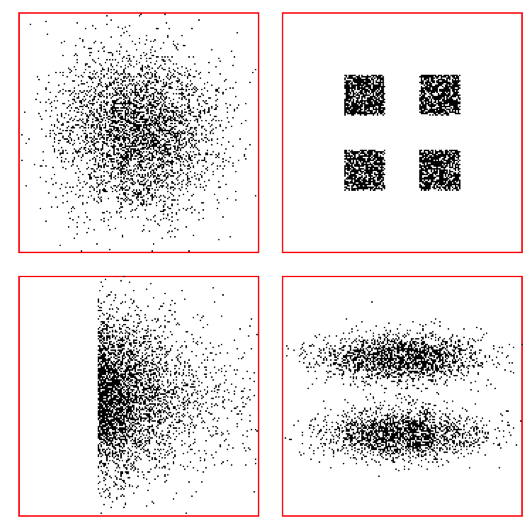
\includegraphics[scale=0.7]{img/Distribuzioni.png}
\caption{Questi quattro dataset hanno statistiche identiche, la stessa media e la stessa matrice di covarianza. }
\label{distribuzioni}
\end{figure}
In Figura \ref{distribuzioni} vengono mostrati quattro dataset differenti che hanno la stessa media e la stessa matrice di covarianza. Ovviamente, le statistiche del secondo ordine non sono in grado di rilevare tutta la struttura dei dati. Se assumiamo che i campioni sono distribuiti secondo una mixtura di $c$ distribuzioni normali, allora possiamo approssimare una grande varietà di situazioni. Ciò significa assumere che i campioni sono rappresentati da una nuvola dalla forma di una ellissoide di varie grandezze e direzioni. Se il numero delle componenti è sufficientemente alto, possiamo approssimare virtualmente qualsiasi distribuzione come mixtura ed usare i parametri della mixtura per descrivere i dati. Purtroppo abbiamo visto che la stima dei parametri di una mixtura non è un problema abbastanza semplice, un altrenativa sarebbe quella di usare una tecnica non parametrica descritta nel capitolo \ref{metodinonparametrici} per stimare le densità di mixture non conosciute, che se accurata, il risultato della stima è certamente una completa descrizione di cosa possiamo apprendere dai dati. Le regioni di alta densità, le quali potrebbero corrispondere a significanti sottoclassi della popolazione, possono essere trovate osservando i picchi della densità stimata.\\

\noindent Se invece l'obiettivo è quello di trovare le sottoclassi, allora una alternativa più diretta è quella di usare la procedura di \emph{clustering}. In breve, la procedura di clusterind produce una descrizione dei dati in termini di gruppi (cluster) di punti che posseggono una forte similarietà. La procedura di clustering formale usa una funzione criterio, come la somma della radice quadrate delle distanze dal centroide. 

\subsection{Similarity Measures}
Una volta descritto il problema di clustering come la procedura intenta a trovare raggruppamtenti  naturali in un insieme di dati, siamo obbligati a definire cosa intendiamo per raggruppamento naturale. Per quale motivo possiamo dire che i campioni di un cluster sono più simili tra loro rispetto a quelli di un altro cluster? Queste domande portano a die problemi separati:
\begin{itemize}
\item Come si dovrebbe misurare la similarietà tra i campioni?
\item Come si dovrebbe valutare il partizionamento di un insieme di campioni in clusters?
\end{itemize}
In questa sezione di occupiamo del primo dei due problemi.\\

\noindent La più importante misura di similarietà tra due campioni è la distanza fra loro. Un modo per incominciare l'investigazione è quello di definire una metrica di riferimento adeguata e calcolare la matrice delle distanze tra tutte le coppie di campioni. Se la distanza è una buona misura di dissimilarietà allora dobbiamo aspettarci che la distanza tra i campioni dello stesso cluster è significativamente minore rispetto alla distanza di campioni appartenenti a cluster differenti. Supponiamo per un momento che la distanza euclidea fra due campioni dello stesso cluster deve essere minore di una soglia che indichiamo con $d_0$, è ovvio che la scelta di $d_0$ è molto importante, se $d_0$ è molto grande, allora tutti i campioni verranno assegnati ad un solo cluster, viceversa, se $d_0$ è molto piccolo ogni campione resterà isolato. Per ottenere u raggruppamento naturale, $d_0$ dovrà essere maggiore della distanza intra-cluster (\emph{within cluster}) e minore della distanza fra cluster (\emph{between-cluster})(Fig.\ref{similarieta}).\\
 
\begin{figure}
\centering
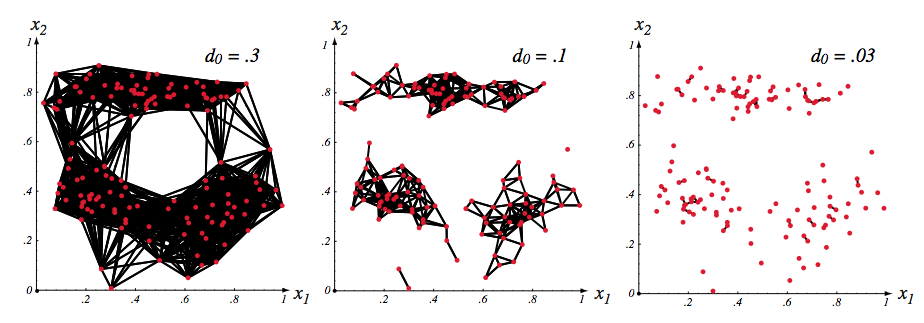
\includegraphics[scale=0.45]{img/similarieta.png}
\caption{Esempio di clustering basato sulla distanza come misura di similarietà}
\label{similarieta}
\end{figure}

\noindent Meno evidente è forse il fatto che i risultati del clustering dipendono dalla scelta di una distanza euclidea come misura di dissimilarietà. Questa particolare scelta è giustificata se lo spazio delle caratteristiche è isotropico ed i dati sono distribuiti uniformemente lungo tutte le direzioni, i cluster definiti secondo questo criterio sono invarianti per traslazione o rotazione. Invece non sono invarianti a trasformazioni lineari oppure a trasformazioni che distorciono le relazioni di distanza. 
\begin{figure}
\centering
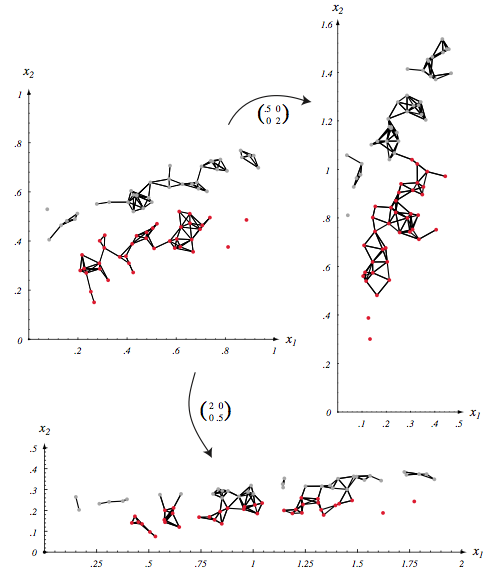
\includegraphics[scale=0.8]{img/similarieta1.png}
\caption{}
\label{similarieta1}
\end{figure}
In figura \ref{similarieta1} c'è un esempio di scaling degli assi, possiamo osservare i differenti raggruppamenti dei dati. Un modo per ottenere l'invarianza è quello di normalizzare i dati. Per esempio, per ottenere l'invarianza per lo spostamento o scaling degli assi si potrebbe traslare e scalare gli assi in modo tale da standardizzare i dati, quindi con media zero e varianza unitaria. Invece per ottenere l'invarianza per rotazione un metodo potrebbe essere quello di ruotare gli assi in modo tale da farli coincidere con gli autovettori della matrice di covarianza. Un alternativa allo scaling degli assi invece potrebbe essere quella di considerare altre metriche. Per esempio una potrebbe essere del tipo
\begin{equation}
d(\mathbf{x}, \mathbf{x}') = \left( \sum_{k=1}^d \abs{x_k - x_k'}^q \right)^{1/q} 
\end{equation}
dove $q \geq 1$ è un parametro. Impostando $q=2$ otteniamo proprio la distanza euclidea mente con $q=1$ otteniamo la distanza di \emph{Manhattan} o \emph{city block}. C'è da notare che soltanto con $q=1$ è invariante per rotazione e traslazione. Un altra alternativa è quella di usare alcuni tipi di metriche basate sui dati stessi, come la distanza di \emph{Mahalanobis}.\\

\noindent Più in generale, si potrebbe abbandonare il criterio basato sulla distanza ed introdurre un criterio basato su una funzione di similarietà $s(\mathbf{x}, \mathbf{x}')$ per paragonare i due vettori $\mathbf{x}$ ed $\mathbf{x}'$. Convenzionalmente, questa è una funzione simmetrica i cui valori sono grandi quando i due vettori sono simili. Per esempio l'angolo tra i due vettori è un importante misura della loro similarietà, quindi la normalizzazione del prodotto interno
\begin{equation}\label{50}
s(\mathbf{x}, \mathbf{x}') = \frac{\mathbf{x}^t\mathbf{x}'}{\norma{\mathbf{x}} \norma{\mathbf{x}'}}
\end{equation}
potrebbe essere un appropriata funzione di similarietà. Questa misura, che è il coseno dell'angolo tra i due vettori, è invariante per rotazione e dilatazione nonstante non sia invariante per traslazione e per le trasformazioni lineari in generale. \\

\noindent Quando le caratteristiche sono valori binari (0 o 1) la funzione di similarietà (Eq. \ref{50}) ha una semplice intrepretazione in termini di caratteristiche condivise. Diciamo che un campione $\mathbf{x}$ possiede l' \emph{i}-esimo attributo se $x_i=1$. Allora $\mathbf{x}^t\mathbf{x}'$ è semplicemente il numero di attributi posseduti da $\mathbf{x}$ e $\mathbf{x}'$, e $\norma{\mathbf{x}} \norma{\mathbf{x}'} = (\mathbf{x}^t \mathbf{xx}'^t \mathbf{x}')^{1/2}$ è la media geometrica del numero di attributi posseduti da $\mathbf{x}$ e da $\mathbf{x}'$. Così, $s(\mathbf{x}, \mathbf{x}')$ è una misura relativa agli attributi posseduti in comune. Alcune semplici variazioni sono
\begin{equation}
s(\mathbf{x}, \mathbf{x}') = \frac{\mathbf{x}^t \mathbf{x}'}{d}
\end{equation}
che sono gli attributi condivisi, e
\begin{equation}
s(\mathbf{x}, \mathbf{x}') = \frac{\mathbf{x}^t \mathbf{x}'}{\mathbf{x}^t \mathbf{x} + \mathbf{x}'^t \mathbf{x}' - \mathbf{x}^t \mathbf{x}'} 
\end{equation}
che è il rapporto tra il numero di attributi condivisi ed il numero di attributi posseduti da $\mathbf{x}$ o da $\mathbf{x}'$. Questa misura è nota come distanza di Tanimoto ed è frequentemente incontrata nel campo di \emph{information retrival}.
 
\section{Criterion Functions For Clustering}
Abbiamo appena considerato il primo dei problemi del clustering cioè quello di come misurare la similarietà. Adesso ci occuperemo del secondo problema quindi una funzione criterio che deve essere ottimizzata. Supponiamo che abbiamo un insieme $\mathcal{D}  = { \mathbf{x}_1, \dots, \mathbf{x}_n }$ di $n$ campioni che devono essere partizionati in $c$ sottoinsimemi $\mathcal{D}_1, \dots, \mathcal{D}_c$. Ogni sottoinsieme rappresenta un cluster, ed i campioni appartenenti allo stesso cluster sono in qualche modo più simili tra loro rispetto agli altri cluster. Un modo per fare questo è quello di definire una funzione criterio che misura la qualità del clustering. Allora il problema è quello di trovare la partizione che estremizza la funzione criterio.

\subsection{The Sum-of-Squared-Error Criterion}
La funzione criterio più semplice e quella maggiormente usata per il clustering è il \emph{sum-of-squared-error}. Denotiamo con $n_i$ i numero di campioni nei sottoinsimemi $\mathcal{D}_i$ e denotiamo con $\mathbf{m}_i$ le medie di questi campioni, 
\begin{equation}
\mathbf{m}_i = \frac{1}{n_i} \sum_{x \in \mathcal{D}_i} \mathbf{x}
\end{equation}
Allora la \emph{sum-of-squared-error} è definita mediante la seguente formula
\begin{equation}
J_e = \sum_{i=1}^c \sum_{x \in \mathcal{D}_i} \norma{\mathbf{x} - \mathbf{m}_i}^2
\end{equation}
Questa funzione criterio ha una semplice interpretazione: Dati i cluster $\mathcal{D}_i$, il vettore media $\mathbf{m}_i$ è quello che meglio rappresenta i campioni in $\mathcal{D}_i$ nel senso che minimizza la somma delle radici quadrate della distanza $\mathbf{x}-\mathbf{m}_i$. Così, $J_e$ misura l'errore totale rappresentato dagli $n$ campioni $\mathbf{x}_1, \dots, \mathbf{x}_n$ raggruppati in $c$ cluster con centroidi $\mathbf{m}_1, \dots, \mathbf{m}_c$. Il valore di $J_e$ dipende da come i campioni sono raggruppati in cluster e dal numero di cluster. La partizione ottima è definita quando $J_e$ è minimo, clustering di questi tipo sono spesso chiamati partizioni a minima varianza, si potrebbe andare incontro a problemi quando tra i cluster c'è una grande differenza in base al numero di campioni, in questo caso può succedere che potrebbero esserci problemi nella partizione come  mostra la figura \ref{cluster}.
\begin{figure}
\centering
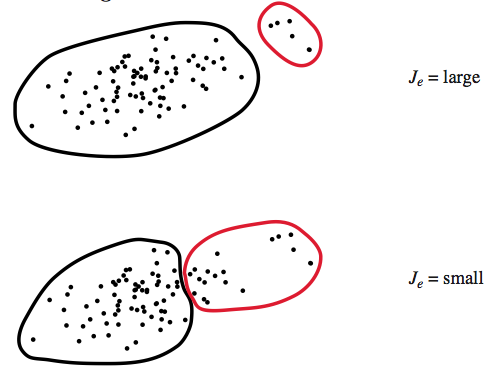
\includegraphics[scale=0.5]{img/cluster.png}
\caption{}
\label{cluster}
\end{figure}
 
\section{Iterative Optimization}
Una volta che la funzione criterio è stata selezionata, il clustering diventa un problema ben definito come ottimizzazione discreta: Trovare le partizioni di un insieme di campioni che estremizzano la funzione criterio. Poichè l'insieme dei campioni è finito, ci sono quindi soltanto un numero finito di partizioni, così, il problema può essere sempre risolto con una enumerazione esaustiva, ma la complessità computazionale di un algoritmo rende tale approccio impensabile. Ci sono approssimativamente $c^n /c!$ modi di partizionare un insieme di $n$ elementi in $c$ sottoinsiemi, ed il fatto che dipende esponenziamente da $n$ è schiacciante. Per esempio una ricerca esaustiva del partizionamento di 100 campioni in 5 cluster richiede più di $10^{67}$ partizionamenti. \\

\noindent L'approccio più frequentemente usato nel cercare un partizionamento ottimo è un ottimizzazione iterativa. L'idea di base è quella di trovare delle partizioni iniziali e muovere i campioni da un gruppo all'altro in modo tale da migliorare i valori della funzione criterio.  In genere questi approcci garantiscono un ottimizzazione locale ma non globale, inoltre c'è da considerare che differenti punti di inizio portano a soluzioni differenti e non si può mai sapere se è stata trovata la migliore soluzione. Nonostante queste limitazioni, il fatto che la complessità computazionale è sopportabile fa di esso un approccio attrattivo.\\

\noindent Consideriamo l'uso di un miglioramento iterativo per minimizzare il criterio \emph{sum-of-squared-error} $J_e$, scritto come
\begin{equation}
J_e = \sum_{i=1}^c J_i
\end{equation}
dove l'errore effettivo per cluster è definito nel seguente modo
\begin{equation}
J_i = \sum_{\mathbf{x} \in \mathcal{D}_i} \norma{\mathbf{x}-\mathbf{m}_i}^2
\end{equation}
e la media di ogni cluster è come prima
\begin{equation}
\mathbf{m}_i = \frac{1}{n_i} \sum_{\mathbf{x} \in \mathcal{D}} \mathbf{x}
\end{equation}
Supponiamo che il campione $\hat{\mathbf{x}}$ è attualmente nel cluster $\mathcal{D}_i$ e si tenta di spostarlo nel cluster $\mathcal{D}_j$. Allora $\mathbf{m}_j$ cambia
\begin{equation}
\mathbf{m}_j^* = \mathbf{m}_j + \frac{\hat{\mathbf{x}}-\mathbf{m}_j}{n_j+1}
\end{equation}
e $J_j$ si incrementa
\begin{equation}
J_j^* = \sum_{\mathbf{x} \in \mathcal{D}_j} \norma{\mathbf{x} - \mathbf{m}_j^*}^2 + \norma{\hat{\mathbf{x}} - \mathbf{m}_j^*}^2
\end{equation}
effettuando gli opportuni calcoli
\begin{equation}
\begin{split}
J_j^* &= \sum_{\mathbf{x} \in \mathcal{D}_j} \norma{\mathbf{x} - \mathbf{m}_j^*}^2 + \norma{\hat{\mathbf{x}} - \mathbf{m}_j^*}^2\\
&= \left(  \sum_{\mathbf{x} \in \mathcal{D}_i} \left|\left| \mathbf{x} - \mathbf{m}_j - \frac{\hat{\mathbf{x}}-\mathbf{m}_j}{n_j+1} \right| \right|^2   \right) + \left| \left|  \frac{n_j}{n_j +1} (\hat{\mathbf{x}} - \mathbf{m}_j)  \right| \right|^2 \\
&= J_j + \frac{n_j}{n_j+1}\norma{\hat{\mathbf{x}} - \mathbf{m}_j}^2
\end{split}
\end{equation}
Sotto l'assunzione che se $n_i \neq 1$ allora $\mathbf{m}_i$ cambia in
\begin{equation}
\mathbf{m}_i^* = \mathbf{m}_i - \frac{\hat{\mathbf{x}} - \mathbf{m}_i }{n_j-1}
\end{equation}
e $J_i$ si decrementa 
\begin{equation}
J_i^* = J_i - \frac{n_i}{n_i-1} \norma{\hat{\mathbf{x}} - \mathbf{m}_i}^2
\end{equation}
Queste equazioni semplificano notevolmente il calcolo delle variazioni nella funzione criterio. Spostare $\hat{\mathbf{x}}$ da $\mathcal{D}_i \ \text{a} \ \mathcal{D}_j$ è un vantaggio se il decremento i $J_i$ è maggiore dell'incremento in $J_j$. Questo il caso in cui
\begin{equation}
\frac{n_i}{n_i-1} \norma{\hat{\mathbf{x}} - \mathbf{m}_i}^2 > \frac{n_j}{n_j+1} \norma{\hat{\mathbf{x}} -\mathbf{m}_j }^2
\end{equation}
il che tipicamente succede quando $\hat{\mathbf{x}}$ è più vicino ad $\mathbf{m}_j$ che ad $\mathbf{m}_i$. Se il riassegnamento è redditizio, allora il maggiore decremento della somma degli errori al quadrato è ottenuto selezionando il cluster per il quale $n_j \norma{\hat{\mathbf{x}} - \mathbf{m}_j}^2/(n_j+1)$ è minimo. Questo posta alla seguente procedura di clustering:

\begin{codebox}
\Procname{$\proc{Basic Iterative Minimum-Squared-Error Clustering}$}
\li \textbf{begin initialize} $n, c, \mathbf{m}_1, \mathbf{m}_2, \dots, \mathbf{m}_c$
\li 	\Do seleziona casualmente il campione $\hat{\mathbf{x}}$
\li		$i \gets \arg \min{i} \norma{\mathbf{m}_{i'}- \hat{\mathbf{x}} }$
\li	\If $n_i \neq 1$	
\li 		\Then calcola
\li              
		$\rho_j=
		\begin{cases}
		\frac{n_i}{n_i+1} \norma{\hat{\mathbf{x}} - \mathbf{m}_i}^2 & \ \ \ \ \ j \neq i\\
		\frac{n_i}{n_i-1} \norma{\hat{\mathbf{x}} - \mathbf{m}_i}^2 &  \ \ \ \ \ i = j 
		\end{cases}$ 		
\li		\If $\rho_k \leq \rho_j  \ \text{per ogni} \ j$
\li			\Then trasferisci $\hat{\mathbf{x}} \ \text{in} \ \mathcal{D}_k$
\li				 ricalola $J_e, \mathbf{m}_i, \mathbf{m}_k$
		\End 
\li	\Until non si ha nessun cambiamenti di $J_i$ in $n$ tentativi	
	\li \Return $\mathbf{m}_1, \mathbf{m}_2, \dots, \mathbf{m}_c$	
	\End
	\End
\li \textbf{end}	
\end{codebox}
Questa procedura è essenzialmente una versione sequenziale della procedura $k$-means descritta nella sezione precedente. Nel caso del $k$-means si aspettava finchè tutti gli $n$ campioni venivano classificati prima dell'aggiornamento, mentre la procedura Iterativa Minimum-Squared-Error aggiorna dopo che ogni campione è stato riclassificato. Questa è una procedura graduale ottimale e può essere facilmente modificata per applicarla  a problemi nei quali i campioni sono acquisiti sequenzialmente e quindi il clustering potrebbe essere fatto in modo \emph{on-line}.   

\section{Hierarchical Clustering}


\subsection{Definitions}
Consideriamo di voler partizionare $n$ campioni in $c$ cluster. Se incominciamo con $n$ cluster allora ogni cluster è formato da un unico campione. La prossima partizione la effettuiamo in $n-1$ cluster, poi ancora in $n-2$ e così via, finchè tutti i campioni formino un unico cluster. Si può affermare che siamo al livello $k$ della sequenza quando $c = n-k+1$.  Così facendo, il livello uno corrisponde ad $n$ cluster ed il livello $n$ corrisponde ad un unico cluster. Dati due campioni $\mathbf{x}$ e $\mathbf{x}'$ situati allo stesso livello allora potranno essere raggruppati insieme nello stesso cluster. Se questo processo ha la propietà che se due campioni appartengono allo stesso cluster al livello $k$ e rimangono insieme per tutti i livelli più alti, allora questo processo è detto \emph{hierarchical clustering} (clustering gerarchico).\\

\noindent La più naturale rappresentazione del clustering gerarchico è un albero chiamato dendogramma, il quale mostra come i campioni sono stati raggruppati. 
\begin{figure}
\centering
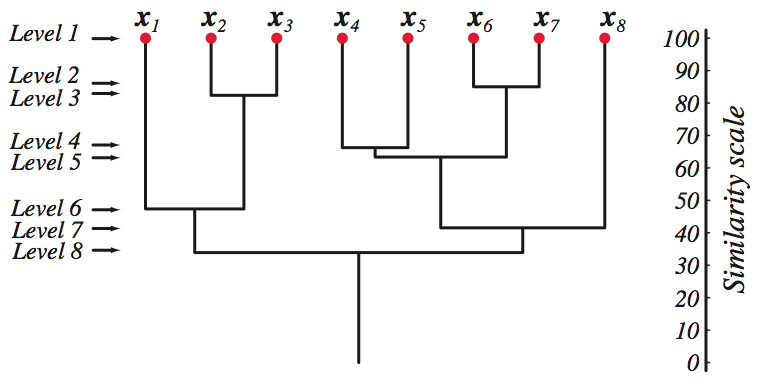
\includegraphics[scale=0.5]{img/dendogramma.png}
\caption{Esempio di dendogramma}
\label{dendogramma}
\end{figure}
In figura \ref{dendogramma} è stato mostrato un dendogramma per un problema semplice con otto campioni. Al livello $k=1$ ogni singolo campione rappresenta un cluster. Al livello $k=2$, $\mathbf{x}_6$ ed $\mathbf{x}_7$ sono stati raggruppati in un cluster e staranno insieme nello stesso cluster fino alla fine. Se è possibile misurare delle similarietà tra i cluster allora il dendogramma è generalmente disegnata con un scala che indica la similarietà tra i cluster che sono stati raggruppati.\\

\noindent Ci sono anche altre rappresentazioni del clustering gerarchico, come l'uso degli insiemi e quindi dei diagrammi di Venn oppure una rappresentazione utilizzando le parentesi graffe per indicare gli insiemi. Ma il dendogramma resta sempre il metodo preferito.\\

\noindent Data la sua semplicità, il clustering gerarchico è una tecnica molto usata nel metodo \emph{unsupervised}. La stessa procedura, inoltre può essere divisa in due distinti approcci. L'approccio Agglomerativo (bottom-up), questa procedura inizia da $n$ cluster composti da un sono campione e poi effettua una fusione tra cluster. L'altro approccio definito $\emph{Divisive}$ è top-down, ed è l'inverso del precedente, quindi si parte da un unico cluster per poi dividere in cluster più piccoli. 

\subsection{Agglomerative Hierarchical Clustering}
I passi più importanti della procedura agglomerativa sono contenuti nel seguente algoritmo, dove $c$ è il numero di cluster finale
\begin{codebox}
\Procname{$\proc{Agglomerative Hierarchical Clustering}$}
\li \textbf{begin initialize} $c, \hat{c} \gets n, \mathcal{D}_i \gets \{ \mathbf{x}_i \}, i=1,\dots, n$
\li	\Do $\hat{c} \gets \hat{c} - 1$
\li		trova il cluster più vicino, $\mathcal{D}_i \ \text{e} \ \mathcal{D}_j$
\li		fondi $\mathcal{D}_i$ e $\mathcal{D}_j$
	\End
\li	\Until	 $c=\hat{c}$
\li	\Return $c$ clusters
\li \textbf{end}	
\end{codebox}
Come descritto sopra, qeusta procedura termina quando è stato ottenuto il numero di cluster specificato. Se si continua fino a $c=1$ allora si ottiene proprio il dendogramma. A qualsiasi livello la distanza tra i cluster più vicini può fornire il valore di dissimilarietà a quel livello. Da notare che non è stata introdotta come viene misurata la distanza tra clusters ed è interessata la linea $3$ dell'algoritmo. Le considerazioni sono molto simili alle funzioni criterio utilizzate nel criterio generale. Per semplicità focalizziamo l'attenzione sulle seguenti misure di distanza
\begin{gather}
d_{min}(\mathcal{D}_i, \mathcal{D}_j) = \min_{\mathbf{x} \in \mathcal{D}_i, \mathbf{x}' \in \mathcal{D}_j} \norma{\mathbf{x} - \mathbf{x}'}\\
d_{max}(\mathcal{D}_i, \mathcal{D}_j) = \max_{\mathbf{x} \in \mathcal{D}_i, \mathbf{x}' \in \mathcal{D}_j} \norma{\mathbf{x} - \mathbf{x}'} \\
d_{avg}(\mathcal{D}_i, \mathcal{D}_j) = \frac{1}{n_i n_j} \sum_{\mathbf{x} \in \mathcal{D}_i} \sum_{\mathbf{x}' \in \mathcal{D}_j} \norma{\mathbf{x} - \mathbf{x}'}\\
d_{mean}(\mathcal{D}_i, \mathcal{D}_j) = \norma{\mathbf{m}_i - \mathbf{m}_j}  
\end{gather}
Queste misure di similarietà generalmente producono cluster compatti e ben separati.

\paragraph{Nearest-Neighbor Algorithm}
Quando viene usata la funzione $d_{min}(\cdot, \cdot)$ per misurare la distanza tra cluster allora l'algoritmo prende il nome di \emph{Nearest-Neighbor Algorithm} o \emph{minimum algorithm}. Inoltre se l'algoritmo è terminato quando la distanza tra  cluster più vicini eccede un' arbitraria soglia allora è chiamato \emph{single-linkage algorithm}. Supponiamo di immaginare i campioni come nodi di un grafo, con gli \emph{edges} che formano un cammino tra i nodi nello stesso sottoinsieme $\mathcal{D}_i$. Quando viene usata la misura di distanza $d_{min}(\cdot, \cdot)$ la fusione tra $	\mathcal{D}_i$ e $	\mathcal{D}_j$ corrisponde nell'aggiungere un \emph{edge} tra la coppia di nodi più vicina in  $	\mathcal{D}_i$ e $	\mathcal{D}_j$. Poiché il collegamento  avviene sempre tra cluster differenti allora il grafo risultante non è mai un circuito chiuso, ma questa procedura genera un albero. Se invece si continua finché tutti i sottoinsiemi sono connessi allora il risultato è uno \emph{spanning tree}, un albero con un cammino da e verso qualsiasi nodo. Così utilizzando $d_{min}(\cdot, \cdot)$ come distanza di misura, allora la procedura di clustering agglomerativa diventa un algortirmo per generare un \emph{minimal spanning tree}.   
\begin{figure}
\centering
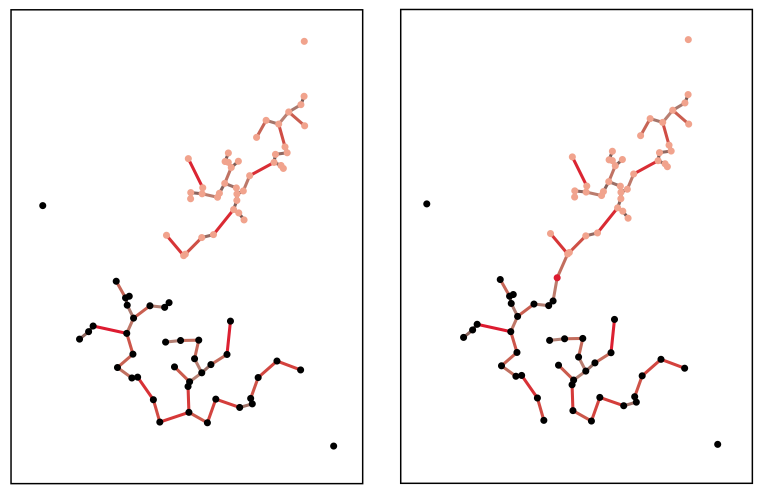
\includegraphics[scale=0.5]{img/spanningtree.png}
\caption{}
\label{spanning}
\end{figure}
In Figura \ref{spanning} sono mostrati i risultati applicando la procedura a dei dati gaussiani. In entrambi i casi la procedura è stata fermata ottenendo così due grandi cluster. Il \emph{minimal spanning tree} può essere ottenuto aggiungendo  l' edge più corto possibile tra i due cluster.

\paragraph{The Farthest-Neighbor Algorithm}
Quando come misura della distanza viene utilizzata $d_{max}(\cdot, \cdot)$ allora l'algoritmo è chiamato \emph{Farthest-Neighbor Algorithm} o \emph{maximum algorithm}. Invece se termina quando la distanza tra i cluster più vicini eccede una soglia arbitraria allora è detto \emph{complete-linkage algorithm}. La procedura può essere vista come la generazione di un grafo nel quale gli edge collegano tutti i nodi di un clsuter. Nella terminologia della teoria dei grafi, ogni cluster costituisce un sottografo completo. La distanza tra due cluster è determinata mediante la più grande distanza tra nodi di due cluster. Quando i cluster più vicini vengono uniti allora il grafo cambia aggiungendo lati tra ogni coppia di nodi dei due cluster. 
\begin{figure}
\centering
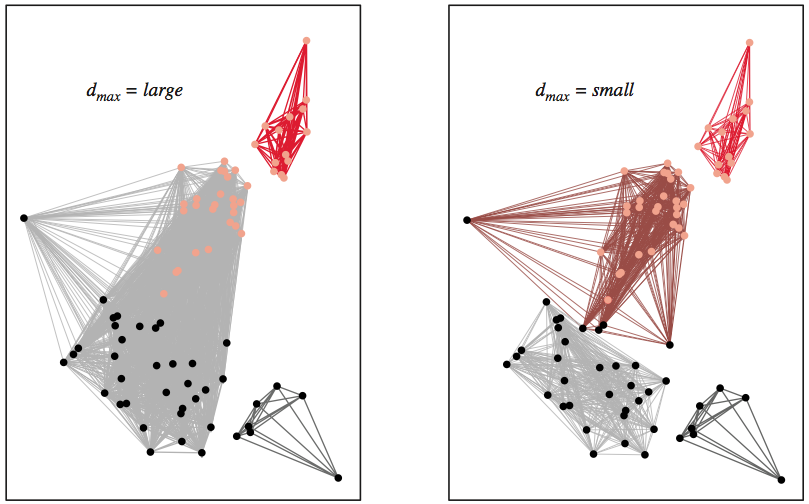
\includegraphics[scale=0.4]{img/grafo2.png}
\caption{}
\label{grafo2}
\end{figure}
In figura \ref{grafo2} è mostrata la tecnica. 

\subsection{Stepwise-Optimal Hierarchical Clustering}
Si specifica il numero di cluster, si pone ogni pattern in un cluster e si ripeteno
\subsection{da completare}

%


%%%%%%%%%%%%%%%%%%%%% chapter.tex %%%%%%%%%%%%%%%%%%%%%%%%%%%%%%%%%
%
% sample chapter
%
% Use this file as a template for your own input.
%
%%%%%%%%%%%%%%%%%%%%%%%% Springer-Verlag %%%%%%%%%%%%%%%%%%%%%%%%%%

\chapter{Chapter Heading}
\label{intro} % Always give a unique label
% use \chaptermark{}
% to alter or adjust the chapter heading in the running head

Your text goes here. Separate text sections with the standard \LaTeX\
sectioning commands.

\section{Section Heading}
\label{sec:1}
% Always give a unique label
% and use \ref{<label>} for cross-references
% and \cite{<label>} for bibliographic references
% use \sectionmark{}
% to alter or adjust the section heading in the running head
Your text goes here. Use the \LaTeX\ automatism for your citations
\cite{monograph}.

\subsection{Subsection Heading}
\label{sec:2}
Your text goes here.

\begin{equation}
\vec{a}\times\vec{b}=\vec{c}
\end{equation}

\subsubsection{Subsubsection Heading}
Your text goes here. Use the \LaTeX\ automatism for cross-references as
well as for your citations, see Sect.~\ref{sec:1}.

\paragraph{Paragraph Heading} %
Your text goes here.

\subparagraph{Subparagraph Heading.} Your text goes here.%
%
\index{paragraph}
% Use the \index{} command to code your index words
%
% For tables use
%
\begin{table}
\centering
\caption{Please write your table caption here}
\label{tab:1}       % Give a unique label
%
% For LaTeX tables use
%
\begin{tabular}{lll}
\hline\noalign{\smallskip}
first & second & third  \\
\noalign{\smallskip}\hline\noalign{\smallskip}
number & number & number \\
number & number & number \\
\noalign{\smallskip}\hline
\end{tabular}
\end{table}
%
%
% For figures use
%
\begin{figure}
\centering
% Use the relevant command for your figure-insertion program
% to insert the figure file.
% For example, with the option graphics use
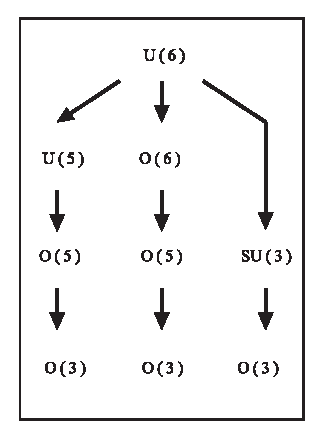
\includegraphics[height=4cm]{figure.eps}
%
% If not, use
%\picplace{5cm}{2cm} % Give the correct figure height and width in cm
%
\caption{Please write your figure caption here}
\label{fig:1}       % Give a unique label
\end{figure}
%
% For built-in environments use
%
\begin{theorem}
Theorem text goes here.
\end{theorem}
%
% or
%
\begin{lemma}
Lemma text goes here.
\end{lemma}
%
%
% Problems or Exercises should be sorted chapterwise
\section*{Problems}
\addcontentsline{toc}{section}{Problems}
%
% Use the following environment.
% Don't forget to label each problem;
% the label is needed for the solutions' environment
\begin{prob}
\label{prob1}
The problem\footnote{Footnote} is described here. The
problem is described here. The problem is described here.
\end{prob}

\begin{prob}
\label{prob2}
\textbf{Problem Heading}\\
(a) The first part of the problem is described here.\\
(b) The second part of the problem is described here.
\end{prob}



%

%%%%%%%%%%%%%%%%%%%%%% chapter.tex %%%%%%%%%%%%%%%%%%%%%%%%%%%%%%%%%
%
% sample chapter
%
% Use this file as a template for your own input.
%
%%%%%%%%%%%%%%%%%%%%%%%% Springer-Verlag %%%%%%%%%%%%%%%%%%%%%%%%%%

\chapter{Chapter Heading}
\label{intro} % Always give a unique label
% use \chaptermark{}
% to alter or adjust the chapter heading in the running head

Your text goes here. Separate text sections with the standard \LaTeX\
sectioning commands.

\section{Section Heading}
\label{sec:1}
% Always give a unique label
% and use \ref{<label>} for cross-references
% and \cite{<label>} for bibliographic references
% use \sectionmark{}
% to alter or adjust the section heading in the running head
Your text goes here. Use the \LaTeX\ automatism for your citations
\cite{monograph}.

\subsection{Subsection Heading}
\label{sec:2}
Your text goes here.

\begin{equation}
\vec{a}\times\vec{b}=\vec{c}
\end{equation}

\subsubsection{Subsubsection Heading}
Your text goes here. Use the \LaTeX\ automatism for cross-references as
well as for your citations, see Sect.~\ref{sec:1}.

\paragraph{Paragraph Heading} %
Your text goes here.

\subparagraph{Subparagraph Heading.} Your text goes here.%
%
\index{paragraph}
% Use the \index{} command to code your index words
%
% For tables use
%
\begin{table}
\centering
\caption{Please write your table caption here}
\label{tab:1}       % Give a unique label
%
% For LaTeX tables use
%
\begin{tabular}{lll}
\hline\noalign{\smallskip}
first & second & third  \\
\noalign{\smallskip}\hline\noalign{\smallskip}
number & number & number \\
number & number & number \\
\noalign{\smallskip}\hline
\end{tabular}
\end{table}
%
%
% For figures use
%
\begin{figure}
\centering
% Use the relevant command for your figure-insertion program
% to insert the figure file.
% For example, with the option graphics use
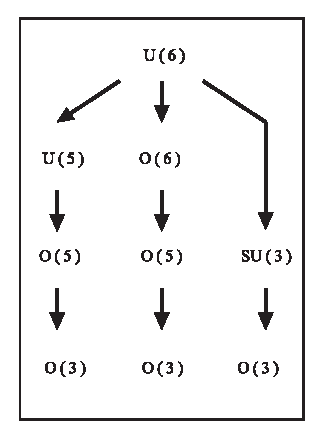
\includegraphics[height=4cm]{figure.eps}
%
% If not, use
%\picplace{5cm}{2cm} % Give the correct figure height and width in cm
%
\caption{Please write your figure caption here}
\label{fig:1}       % Give a unique label
\end{figure}
%
% For built-in environments use
%
\begin{theorem}
Theorem text goes here.
\end{theorem}
%
% or
%
\begin{lemma}
Lemma text goes here.
\end{lemma}
%
%
% Problems or Exercises should be sorted chapterwise
\section*{Problems}
\addcontentsline{toc}{section}{Problems}
%
% Use the following environment.
% Don't forget to label each problem;
% the label is needed for the solutions' environment
\begin{prob}
\label{prob1}
The problem\footnote{Footnote} is described here. The
problem is described here. The problem is described here.
\end{prob}

\begin{prob}
\label{prob2}
\textbf{Problem Heading}\\
(a) The first part of the problem is described here.\\
(b) The second part of the problem is described here.
\end{prob}



%

%\appendix
%\include{appendix}

%%%%%%%%%%%%%%%%%%%%%%%% part.tex %%%%%%%%%%%%%%%%%%%%%%%%%%%%%%%%%%
%
% sample part title
%
% Use this file as a template for your own input.
%
%%%%%%%%%%%%%%%%%%%%%%%% Springer-Verlag %%%%%%%%%%%%%%%%%%%%%%%%%%


\part{Sistemi Adattivi e Reti Neurali}

%%%%%%%%%%%%%%%%%%%%% chapter.tex %%%%%%%%%%%%%%%%%%%%%%%%%%%%%%%%%
%
% sample chapter
%
% Use this file as a template for your own input.
%
%%%%%%%%%%%%%%%%%%%%%%%% Springer-Verlag %%%%%%%%%%%%%%%%%%%%%%%%%%

\chapter{Chapter Heading}
\label{intro} % Always give a unique label
% use \chaptermark{}
% to alter or adjust the chapter heading in the running head

Your text goes here. Separate text sections with the standard \LaTeX\
sectioning commands.

\section{Section Heading}
\label{sec:1}
% Always give a unique label
% and use \ref{<label>} for cross-references
% and \cite{<label>} for bibliographic references
% use \sectionmark{}
% to alter or adjust the section heading in the running head
Your text goes here. Use the \LaTeX\ automatism for your citations
\cite{monograph}.

\subsection{Subsection Heading}
\label{sec:2}
Your text goes here.

\begin{equation}
\vec{a}\times\vec{b}=\vec{c}
\end{equation}

\subsubsection{Subsubsection Heading}
Your text goes here. Use the \LaTeX\ automatism for cross-references as
well as for your citations, see Sect.~\ref{sec:1}.

\paragraph{Paragraph Heading} %
Your text goes here.

\subparagraph{Subparagraph Heading.} Your text goes here.%
%
\index{paragraph}
% Use the \index{} command to code your index words
%
% For tables use
%
\begin{table}
\centering
\caption{Please write your table caption here}
\label{tab:1}       % Give a unique label
%
% For LaTeX tables use
%
\begin{tabular}{lll}
\hline\noalign{\smallskip}
first & second & third  \\
\noalign{\smallskip}\hline\noalign{\smallskip}
number & number & number \\
number & number & number \\
\noalign{\smallskip}\hline
\end{tabular}
\end{table}
%
%
% For figures use
%
\begin{figure}
\centering
% Use the relevant command for your figure-insertion program
% to insert the figure file.
% For example, with the option graphics use
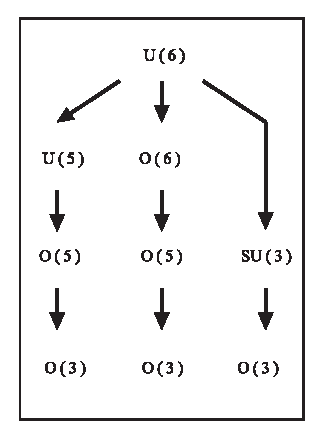
\includegraphics[height=4cm]{figure.eps}
%
% If not, use
%\picplace{5cm}{2cm} % Give the correct figure height and width in cm
%
\caption{Please write your figure caption here}
\label{fig:1}       % Give a unique label
\end{figure}
%
% For built-in environments use
%
\begin{theorem}
Theorem text goes here.
\end{theorem}
%
% or
%
\begin{lemma}
Lemma text goes here.
\end{lemma}
%
%
% Problems or Exercises should be sorted chapterwise
\section*{Problems}
\addcontentsline{toc}{section}{Problems}
%
% Use the following environment.
% Don't forget to label each problem;
% the label is needed for the solutions' environment
\begin{prob}
\label{prob1}
The problem\footnote{Footnote} is described here. The
problem is described here. The problem is described here.
\end{prob}

\begin{prob}
\label{prob2}
\textbf{Problem Heading}\\
(a) The first part of the problem is described here.\\
(b) The second part of the problem is described here.
\end{prob}



%


\backmatter%%%%%%%%%%%%%%%%%%%%%%%%%%%%%%%%%%%%%%%%%%%%%%%%%%%%%%%

\chapter*{Solutions}
\addcontentsline{toc}{chapter}{Solutions}
\markboth{Solutions}{Solutions}

\section*{Problems of Chapter~\ref{intro}}

\begin{sol}{prob1}
The solution is revealed here.
\end{sol}


\begin{sol}{prob2}
\textbf{Problem Heading}\\
(a) The solution of first part is revealed here.\\
(b) The solution of second part is revealed here.
\end{sol}


%%%%%%%%%%%%%%%%%%%%%%%% referenc.tex %%%%%%%%%%%%%%%%%%%%%%%%%%%%%%
% sample references
% "computer science"
%
% Use this file as a template for your own input.
%
%%%%%%%%%%%%%%%%%%%%%%%% Springer-Verlag %%%%%%%%%%%%%%%%%%%%%%%%%%

%
% BibTeX users please use
% \bibliographystyle{}
% \bibliography{}
%
% Non-BibTeX users please use
\begin{thebibliography}{99.}
%
% and use \bibitem to create references.
%
% Use the following syntax and markup for your references
%
% Monographs
\bibitem{monograph} Kajan E (2002)
Information technology encyclopedia and acronyms. Springer, Berlin
Heidelberg New York

% Contributed Works
\bibitem{contribution} Broy M (2002) Software engineering -- From
auxiliary to key technologies. In: Broy M, Denert E (eds)
Software Pioneers. Springer, Berlin Heidelberg New York

% Journal
\bibitem{journal} Che M, Grellmann W, Seidler S (1997)
Appl Polym Sci 64:1079--1090

% Theses
\bibitem{thesis} Ross DW (1977) Lysosomes and storage diseases. MA
Thesis, Columbia University, New York

\end{thebibliography}

\printindex

%%%%%%%%%%%%%%%%%%%%%%%%%%%%%%%%%%%%%%%%%%%%%%%%%%%%%%%%%%%%%%%%%%%%%%

\end{document}





